\chapter{Storing and Using Data} % (fold)
\label{cha:storing_and_using_data}

\begin{quote}
  \Fontlukas\Large
  \renewcommand{\LettrineTextFont}{\relax}
  \lettrine[image=true,lines=3,lraise=0.1]
  {N}{ow} it is time to turn your attention to a the finer details of spell craft. So far the magic you are working has not made use of material components. Fetch the Dragon scales from off the chest in the corner, and place them in that goblet. Prepare you wand, and\ldots
  \ldots
\end{quote}

\bigskip


So far our programs have only been able to work with Literal values. This Chapter introduces new artefacts you can use to store data, and from which you can read the value stored called Variables and Constants. It will also introduce a new artefact that can be used to calculate values called a Function. Using these artefacts you will see how you can store and manipulate values in your code.

When you have understood the material in this chapter you will be able to write code that uses Variable and Constants to stores and manipulates data. You will be able to share data between different Procedures, and create and use Functions to calculate values.

\minitoc

% ========================
% = Concepts - Variables =
% ========================

\clearpage
\section{Concepts Related to Storing and Using Data} % (fold)
\label{sec:concepts_related_to_storing_and_using_data}

Chapter \ref{cha:procedure_declaration}, \nameref{cha:procedure_declaration}, showed you how you can create your own procedures, with each procedure performing a task for the program. The procedures that you created did use some data, but in each case the data was entered directly into the code of the program, as a Literal.

This next step introduces the idea of creating your own artefacts that can be used to \textbf{store}, or \textbf{calculate} a value. Using these artefacts you can start to work with values in a more dynamic way, allowing you to get the computer to perform calculations, and to store and manipulate values.

In this Chapter you will learn how to create the following programming \textbf{artefacts}:
\begin{itemize}
  \item \nameref{sub:variable}: You can \textbf{store} a value in a Variable, and \textbf{retrieve} the value from the Variable.
  \item \nameref{sub:constant}: Is similar to a Variable, except that its value cannot change after it is declared.
  \item \nameref{sub:function}: Is similar to a \nameref{sub:procedure}, but is used to calculate a value rather than to produce a side effect.
\end{itemize}

You will learn about the following \textbf{terminology}:
\begin{itemize}
  \item \nameref{sub:global_variable}: Variables declared within the program's code are called Global Variables.
  \item \nameref{sub:local_variable}: Variables declared within a Function or Procedure are called Local Variables.
  \item \nameref{sub:parameter}: Parameters are variables that allow values to be passed into a Function or Procedure.
  \item \nameref{sub:expressions_with_variables_}: See how Functions, Constant, and Variables can be used in Expressions.
\end{itemize}

Additionally, you will learn how to perform the following \textbf{actions}:
\begin{itemize}
  \item \nameref{sub:assignment_statement}: You use an Assignment Statement to store a value in a Variable.
  \item \nameref{sub:function_call}: This is part of an Expression, and is used to call the Function and to read the returned result.
\end{itemize}

\bigskip

You may need to revise the following programming artefacts:
\begin{itemize}
  \item \nameref{sub:program}: The idea of building your own Programs.
  \item \nameref{sub:procedure}: Creating your own Procedure, as well as calling Procedures from libraries.
\end{itemize}

The following programming terminology will also be used in this Chapter:
\begin{itemize}
  \item \nameref{sub:statement}: An instruction performed in your code.
  \item \nameref{sub:identifier}: The name of an artefact, or the text used to identify something meaningful to the language.
\end{itemize}

This material also requires that you have a good understanding of the following actions:
\begin{itemize}
  \item \nameref{sub:procedure call}: A procedure call is an instruction to run a Procedure.
\end{itemize}

\clearpage

By the end of this material we will have worked through an example where you create a program that calculates change for . This program will read a temperature value in Fahrenheit from the user, and will then output the temperature in Celsius. The output of several runs of this program are shown in Figure \ref{fig:storing-using-simeple-change}.

\begin{figure}[h]
   \centering
   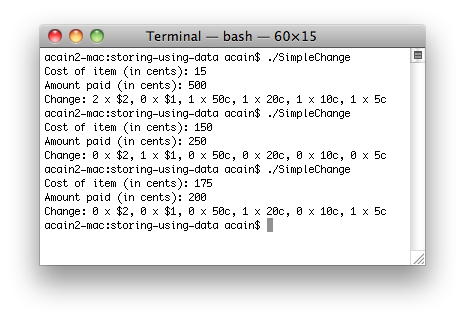
\includegraphics[width=0.9\textwidth]{./topics/storing-using-data/images/SimpleChange} 
   \caption{The Simple Change Calculator running in the Terminal}
   \label{fig:storing-using-simeple-change}
\end{figure}


\clearpage
\subsection{Variable} % (fold)
\label{sub:variable}

A Variable is a \textbf{container} into which you can store a value, which can then be retrieved later. The Variable allows you to store values you want to work with in your program, you store values in the variable so that you can read them back later. The variable's themselves are either a \nameref{sub:global_variable}, \nameref{sub:local_variable}, or \nameref{sub:parameter}.

\begin{figure}[h]
   \centering
   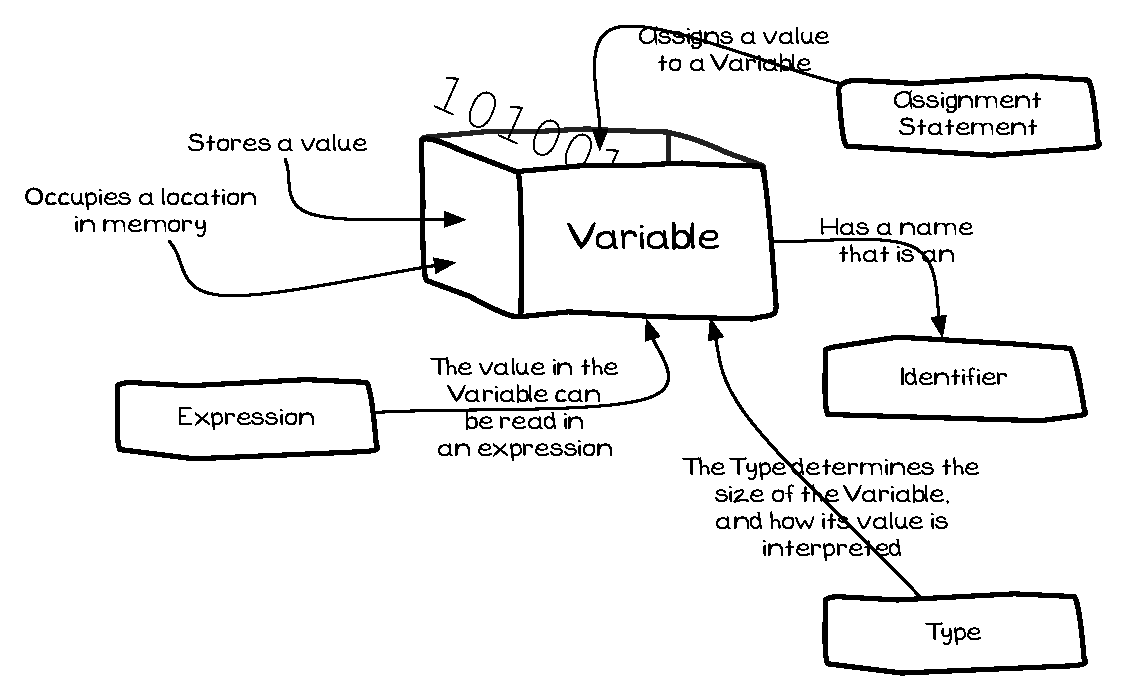
\includegraphics[width=\textwidth]{./topics/storing-using-data/diagrams/Variable} 
   \caption{Variables store a value that can be read and changed}
   \label{fig:storing-using-variable}
\end{figure}

\mynote{
\begin{itemize}
  \item A Variable is an \textbf{artefact}, you can create variables to store values in your programs.
  \item You can think of a Variable like a "box with an item in it". The Variable is the box, its value is the item within it.
  \item Each Variable has a ...
  \begin{itemize}
    \item \textbf{Name} that can be used to refer to it.
    \item \textbf{Value} that it is storing.
    \item \textbf{Type} that determines the size of the Variable and how its value is interpreted.
  \end{itemize}
  \item You use an \nameref{sub:assignment_statement} to store a \emph{value} into the Variable.
  \item You can \textbf{read} the \emph{value} from Variable in Expressions.
  \item The Variable is \textbf{different} to its value:
  \begin{itemize}
    \item The Variable is a container into which a value can be stored.
    \item You can read the \emph{value} from the Variable.
    \item The Variable \textbf{is not} the value, it is a container into which the value is stored.
  \end{itemize}
\end{itemize}
}

% subsection variables (end)
\clearpage
\subsection{Constant} % (fold)
\label{sub:constant}

A Constant is just like a \nameref{sub:variable}, but its value cannot be changed. Constants are declared within the Program, and given a value when they are created. Once they are created the value within the Constant cannot be changed. This is useful for data where you do not want the value changing during the program's execution.

\begin{figure}[h]
   \centering
   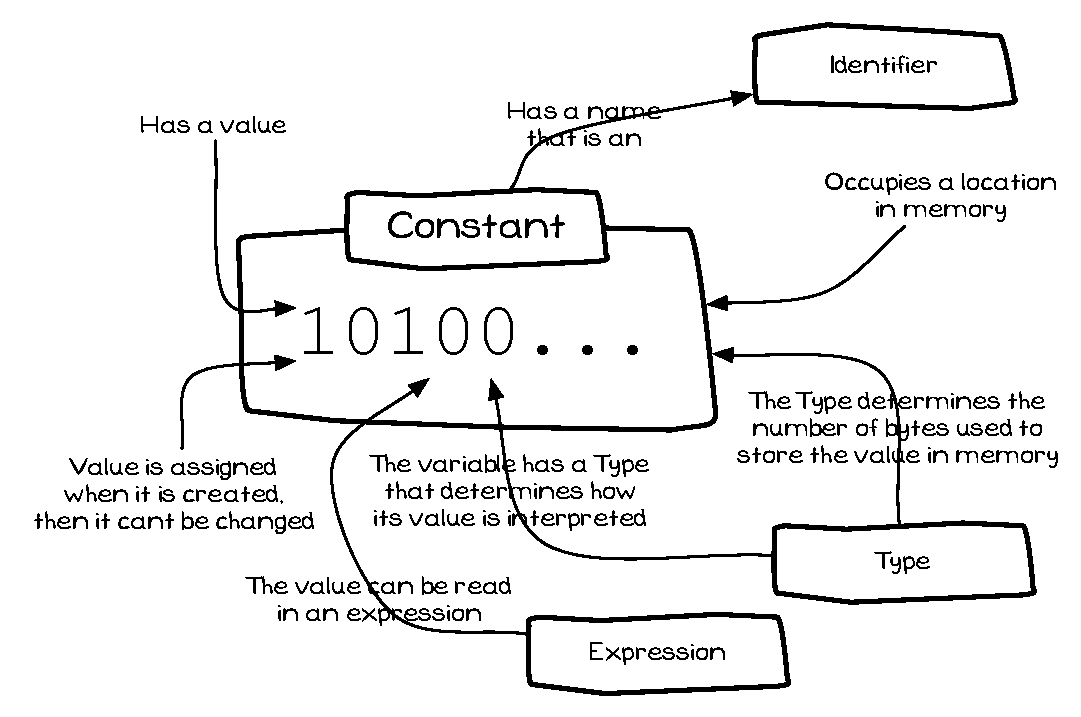
\includegraphics[width=\textwidth]{./topics/storing-using-data/diagrams/Constant} 
   \caption{Constants have a value that cannot be changed}
   \label{fig:constants}
\end{figure}

\mynote{
\begin{itemize}
  \item A Constant is an \textbf{artefact}. You can create Constants in your Program to store values that must not change.
  \item A Constant is similar to a \nameref{sub:variable}, they have a...
  \begin{itemize}
    \item \textbf{Name} that is used to access them.
    \item \textbf{Value} that can be read in an Expression.
    \item \textbf{Type} that determines how their data is interpreted.
  \end{itemize}
  \item You \textbf{read} \emph{values} of Constants in Expressions.
  \item Constants are useful for data you do not want to change during the program. 
  \item The name of the Constant is an \nameref{sub:identifier}.
  \item The Constant's name should reflect the value it is storing.
\end{itemize}
}

% subsection constants (end)
\clearpage
\subsection{Local Variable} % (fold)
\label{sub:local_variable}

Variables can be declared at a number of different places in your code. Variables that are declared within Procedures are called \textbf{Local Variables}. Most of the variables in your code will be Local Variables.

\begin{figure}[h]
   \centering
   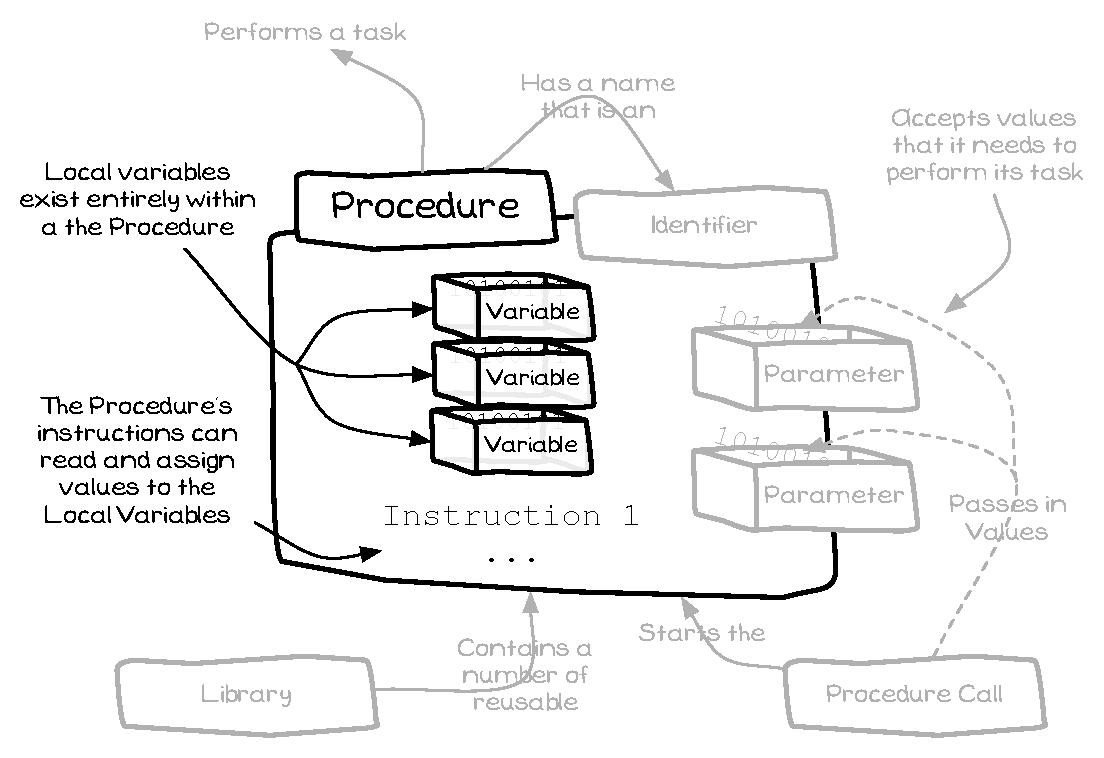
\includegraphics[width=\textwidth]{./topics/storing-using-data/diagrams/LocalVariables} 
   \caption{Variables declared within a Procedure are Local Variables}
   \label{fig:storing-using-data-local-variables}
\end{figure}

\mynote{
\begin{itemize}
  \item Local Variable is the \textbf{term} given to a Variable that is declared within a Procedure.
  \item Variables that are declared within Procedures are called \textbf{Local Variables}.
  \item Local Variables are located \textbf{within} the Procedure they are declared in. 
  \item They can only be accessed by instructions in the Procedure.
  \item It is \textbf{good practice} to use Local Variables to store values. These variables can only be accessed from the instructions within the Procedure, this makes it easier to understand how the variable is being used and where it is being changed. 
  \item Space is allocated for the Local Variables when the Procedure is called.
  \item When the call ends, the Local Variables for that call are destroyed.
\end{itemize}
}

% subsection local_variable (end)
\clearpage
\subsection{Global Variable} % (fold)
\label{sub:global_variable}

Variables and Constants can be declared within a Program. Variables declared in this way are called Global Variables. It seems tempting to use Global Variables to share values between procedures, but this is a bad idea. Global Variables should be avoided, and for many programs are unnecessary. The issue with Global Variables is that their values can be changed from anywhere within the program's code. This can make it difficult to locate the source of errors when globals are used.

While Global Variables should be avoided, Constants should be declared globally. As these values can not change, the issues with Global Variables do not affect Constants. 

\begin{figure}[h]
   \centering
   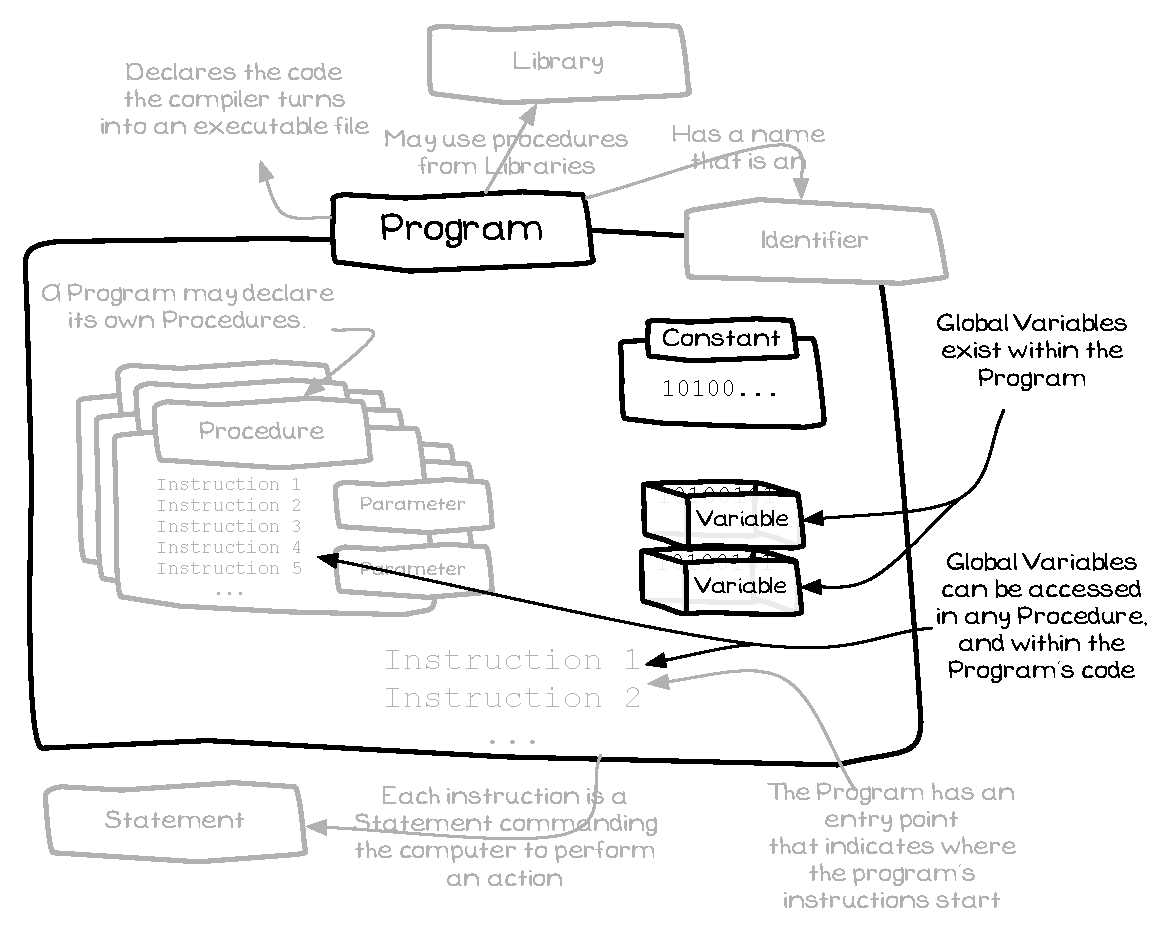
\includegraphics[width=\textwidth]{./topics/storing-using-data/diagrams/GlobalVariables} 
   \caption{Variables declared within a Program are Global Variables}
   \label{fig:storing-using-data-local-variables}
\end{figure}

\mynote{
\begin{itemize}
  \item Global Variable is the \textbf{term} given to a Variable that is declared within the program.
  \item Variables that are declared within a Program are called \textbf{Global Variables}.
  \item Global Variables can be accessed by the program's instructions, and by the instructions in any of the Procedures.
  \item You should \textbf{avoid} using Global Variables. These variables can be accessed anywhere within the Program, making it difficult to locate errors.
  \item Using Global Variables introduces hidden dependencies between Procedures, breaking the isolated nature of the Procedures.
  \item Constants \textbf{should} be declared globally, and used to give meaning to values entered into your code.
  % \item \emph{Magic Numbers} is a term used to describe numeric Literals where the value's meaning is hard to determine. From the perspective of the reader these values are chosen by \emph{magic}. It is poor practice to have \emph{magic numbers}, and these should be replaced by Constants. For example, the value \texttt{42} may appear in code, but what does that mean? If this were called \texttt{BUTTON\_HEIGHT}, its meaning would be known.
\end{itemize}
}

% subsection global_variables (end)
\clearpage
\subsection{Parameter} % (fold)
\label{sub:parameter}

The instructions within a Procedure define the actions that occur when that procedure is called. In most cases these instructions need to be given values to work with. These values can be passed to the Procedure using Parameters. The Parameter is a Variable that has its value set in the Procedure Call.

\begin{figure}[h]
   \centering
   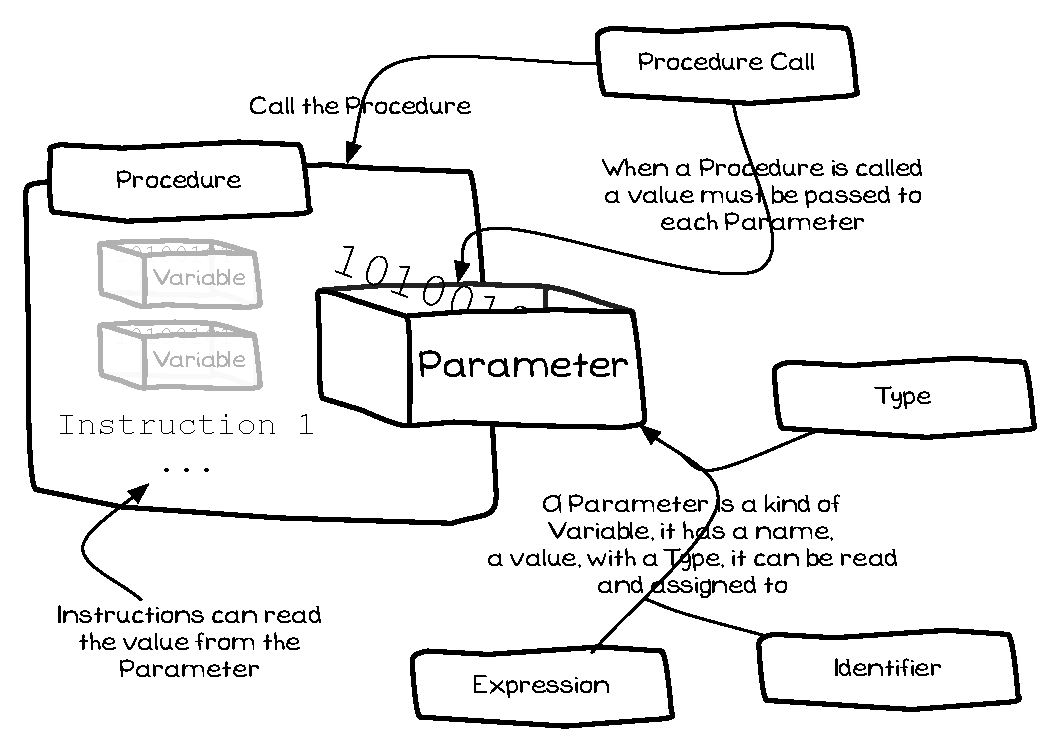
\includegraphics[width=\textwidth]{./topics/storing-using-data/diagrams/Parameter} 
   \caption{Parameters allow data to be passed to Procedures}
   \label{fig:parameters-parameters}
\end{figure}

\mynote{
\begin{itemize}
  \item Parameter is the \textbf{term} given to the Variables declared to accept values passed to Procedures.
  \item The \textbf{Procedure Call} assigns values to each of the Procedure's Parameters.
  \item Parameters allow you to pass values into a Procedure.
  \item Within the Procedure the Parameters can be used in the same way as any other Variable.
  \item It is \textbf{good practice} to use Parameters to pass values into a Procedure.
\end{itemize}
}

% subsection parameters (end)
\clearpage
\subsection{Pass by Value and Pass by Reference} % (fold)
\label{sub:pass_by_value_and_pass_by_reference}

There are actually two ways that values can be passed to Parameters. This relates back to the fact that Variables have two aspects: the Value within the Variable, and the Variable itself. These two means of passing parameters allow you to either pass a value, or pass a Variable.

\begin{figure}[h]
   \centering
   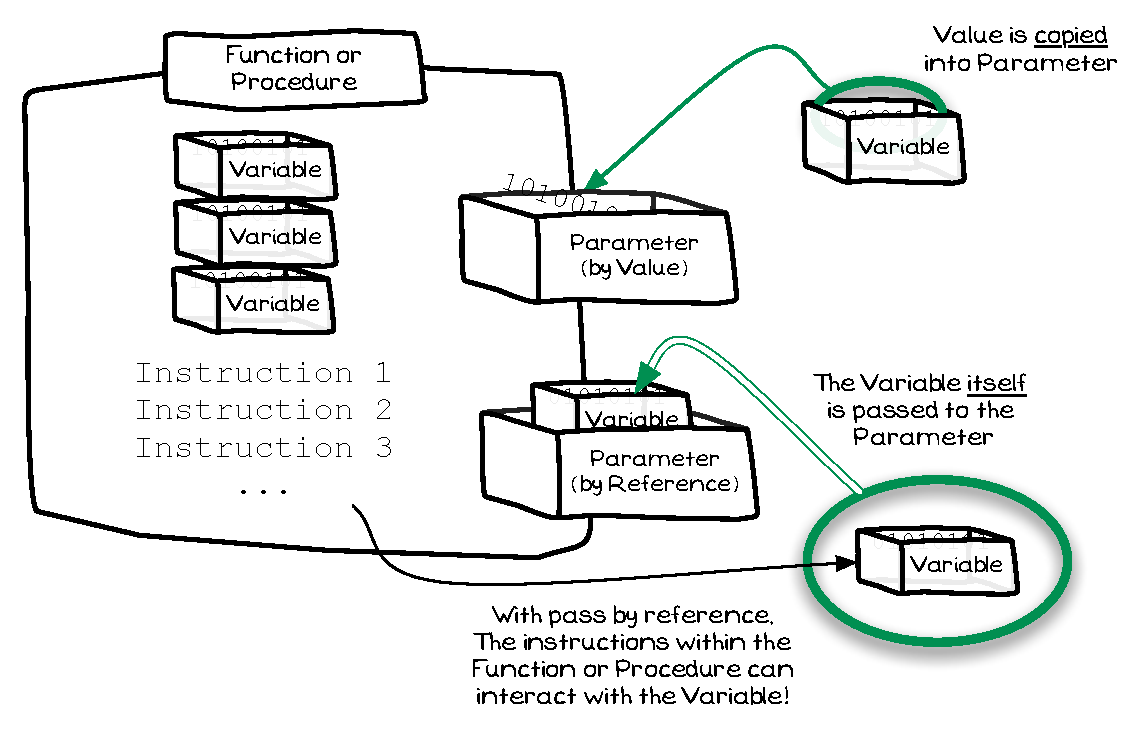
\includegraphics[width=\textwidth]{./topics/storing-using-data/diagrams/ByValByRef} 
   \caption{Parameters can accept data by reference or by value}
   \label{fig:parameters-parameters}
\end{figure}

\mynote{
\begin{itemize}
  \item Pass by Reference and Pass by Value are \textbf{terms} that explain how data is passed to a Parameter.
  \item Most parameters are passed by value.
  \item Pass by value copies the value to the parameter. This means pass by value can work with any Expression.
  \item Pass by reference allows you to pass the Variable itself to the parameter.
  \item The main use for pass by reference is to allow the Procedure or Function to store a value in the Variable passed to the parameter.
  \item It is called pass by reference due to the way it is implemented, with the parameter receiving a reference to the Variable. Section \ref{sec:using_these_concepts_storing_using_data} will cover this in more detail, conceptually the Variable itself is passed to the Parameter.
\end{itemize}
}

% subsection pass_by_reference (end)
\clearpage
\subsection{Statement (with Assignment)} % (fold)
\label{sub:statement_with_assignment_}

Statements are the actions that we can get the computer to perform. At this stage we have covered the statements that run procedures, the \nameref{sub:procedure call}, and the statement to assign values to variables, the \nameref{sub:assignment_statement}.

\begin{figure}[h]
   \centering
   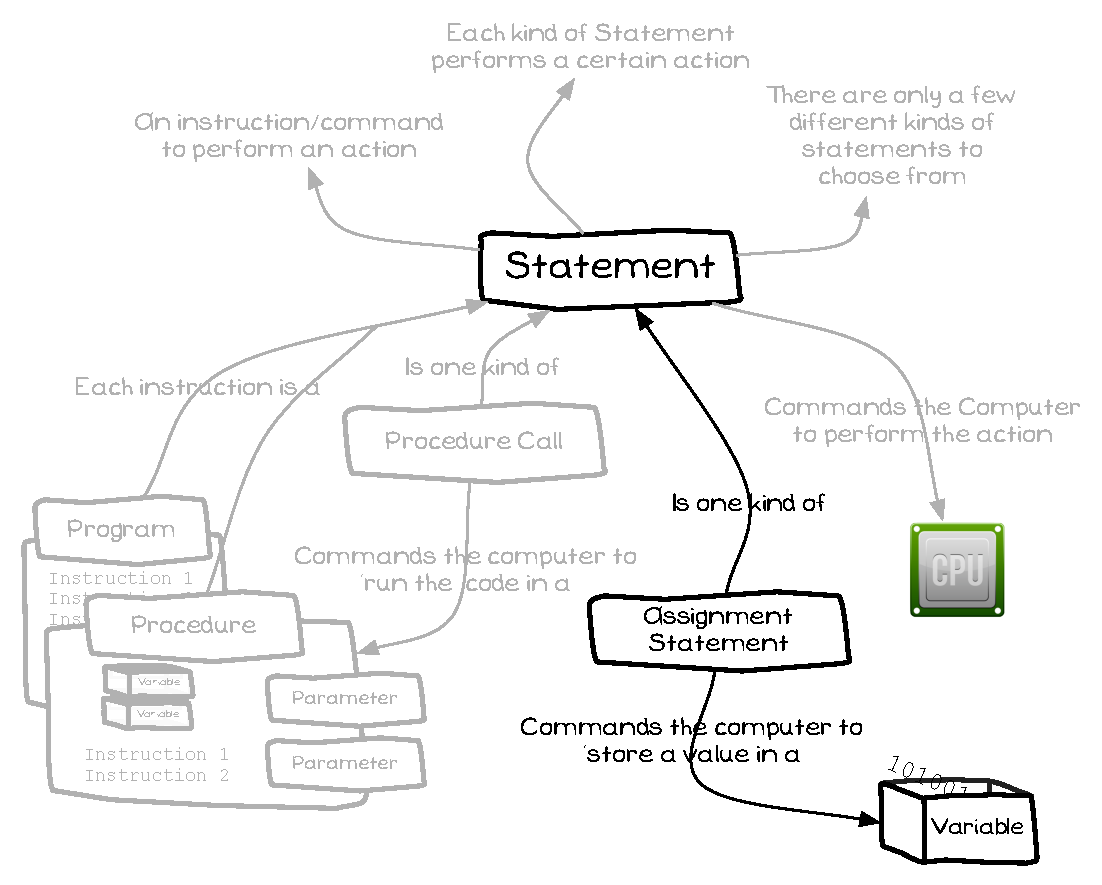
\includegraphics[width=\textwidth]{./topics/storing-using-data/diagrams/Statement} 
   \caption{A Statement may be an Assignment statement}
   \label{fig:storing-using-data-statement}
\end{figure}

\mynote{
\begin{itemize}
  \item Statement is the \textbf{term} given to the instructions in our code.
  \item Statements can be either:
  \begin{itemize}
    \item \nameref{sub:procedure call} used to run the code in a Procedure, as covered in Chapter \ref{cha:program_creation}.
    \item \nameref{sub:assignment_statement} used to calculate a value and store it in a Variable.
  \end{itemize}
  \item All instructions in your code are Statements, these include the instructions in your Program as well as the instructions in your Procedures and Functions.
\end{itemize}
}

% subsection statement_with_assignment_ (end)
\clearpage
\subsection{Assignment Statement} % (fold)
\label{sub:assignment_statement}

The Assignment Statement calculates a value, and stores it in a Variable. You use an assignment statement to store values in variables.

\begin{figure}[h]
   \centering
   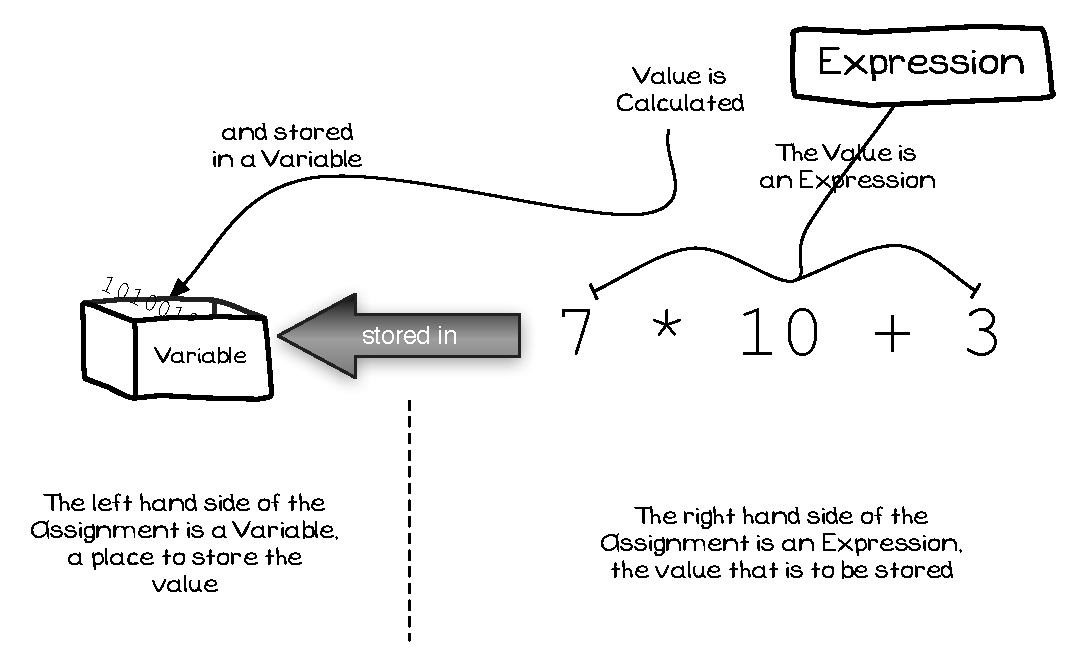
\includegraphics[width=\textwidth]{./topics/storing-using-data/diagrams/AssignmentStatement} 
   \caption{Assignment Statements assign values to Variables}
   \label{fig:storing-using-data-assignment-statement}
\end{figure}

\mynote{
\begin{itemize}
  \item An Assignment Statement is an \textbf{action} you can get the computer to perform.
  \item The \emph{right hand side} of the Assignment is an \textbf{Expression} that calculates the value to be stored.
  \item The \emph{left hand side} of the Assignment is a \textbf{Variable} into which the value is stored.
  \item When the Assignment Statement is executed the Expression is evaluated first, and then the resulting value is stored in the variable.
  \item Its important to remember that the Variable is a location at which to store a value. When the Variable appears on the left hand side of an assignment it is being use to store the resulting value. If the variable appears on the right hand side its value is being used as part of the expression. 
\end{itemize}
}

% subsection assignment_statement (end)
\clearpage
\subsection{Function} % (fold)
\label{sub:function}

Functions are used to calculate values. In many ways a Function is just like a Procedure, it has a name, can be called, can accept parameters, can have local variables, and performs a number of instructions when it is called. Unlike a Procedure, however, Functions are used to calculate values. When the function you called ends it returns back to you with a value.

\begin{figure}[h]
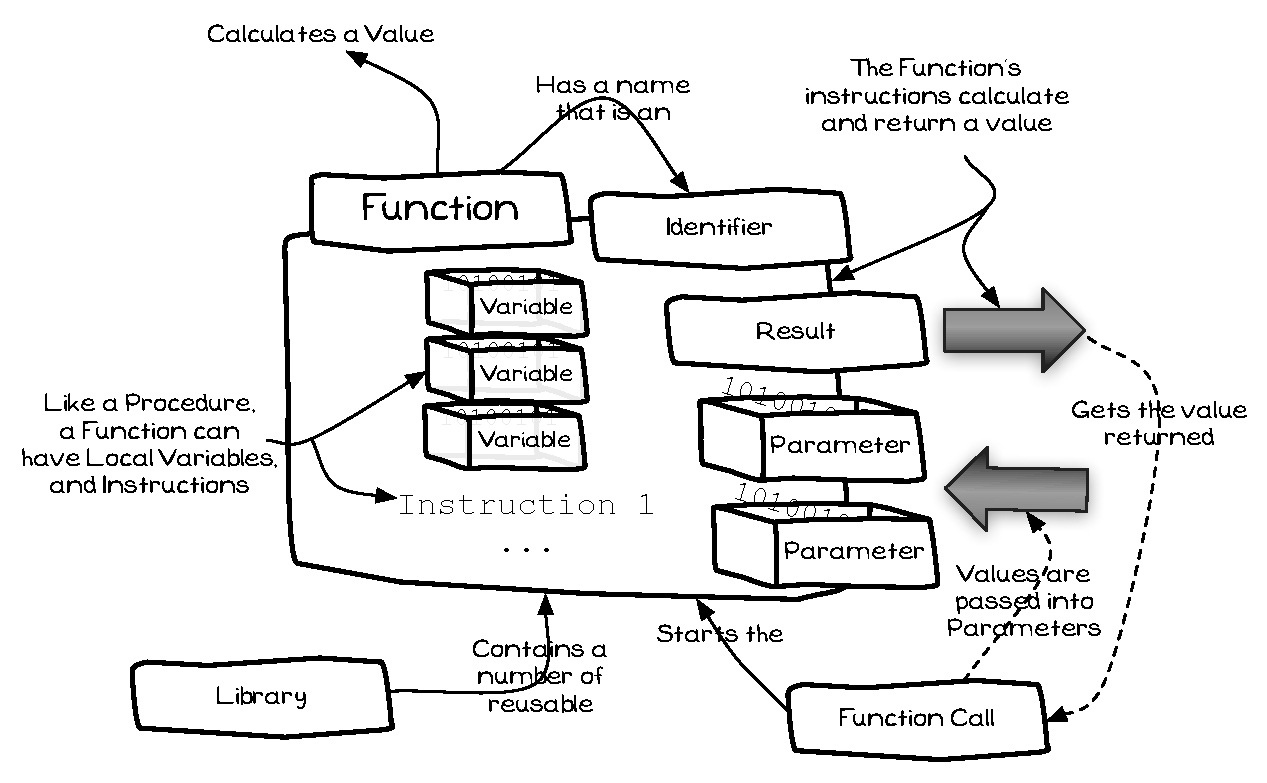
\includegraphics[width=\textwidth]{topics/storing-using-data/diagrams/Function} 
 \caption{A Function is just like a Procedure, except it calculates and returns a Value}
 \label{fig:function-decl-function}
\end{figure}

\mynote{
\begin{itemize}
  \item A Function is an \textbf{Artefact}. Something that you can create and use in your program's code.
  \item A Function is just like a Procedure in that it ...
  \begin{itemize}
    \item Has a name that is used to call it.
    \item Performs instructions when it is executed.
    \item Can accept Parameters to allow the caller to pass in values.
    \item Is allowed to create its own local variables.
  \end{itemize}
  \item Unlike a Procedure, a Function...
  \begin{itemize}
    \item Should \textbf{not} have any side effects.
    \item Calculates and returns a value.
    \item Is called as part of an Expression.
  \end{itemize}
  \item You use Functions to calculate values.
  \item You use a \nameref{sub:function_call} to call a function as part of an Expression.
\end{itemize}
}

% subsection function (end)
\clearpage
\subsection{Function Call} % (fold)
\label{sub:function_call}

A Function Call is used to execute a \nameref{sub:function}, and to read the value that is returned. This is similar to a \nameref{sub:procedure call}, but unlike a procedure call it must be done as part of an Expression.

\begin{figure}[h]
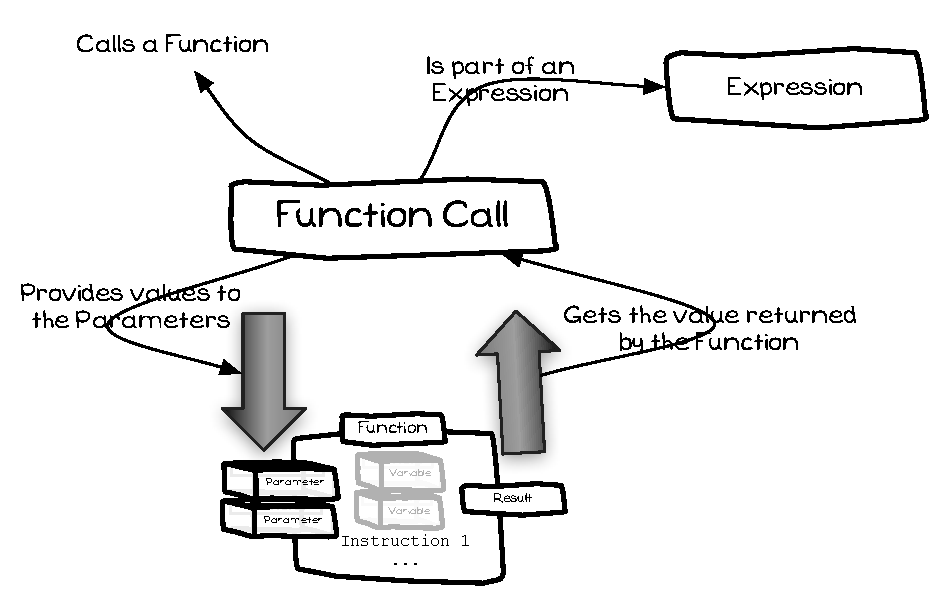
\includegraphics[width=\textwidth]{topics/storing-using-data/diagrams/FunctionCall} 
 \caption{A Function Call is part of an Expression where the value is calculated}
 \label{fig:storing-using-data-function-call}
\end{figure}

\mynote{
\begin{itemize}
  \item A Function Call is an \textbf{action}, but one that is performed as part of an Expression.
  \item Function calls can appear in \emph{any} expression. For example, you can use a Function Call to calculate the value in an \nameref{sub:assignment_statement}. You can use a Function Call to calculate the argument values for a procedure call.
\end{itemize}
}


% subsection function_call (end)
\clearpage
\subsection{Expressions (with Function Calls, Variables, and Constants)} % (fold)
\label{sub:expressions_with_variables_}

You can \textbf{read} the values from Variables and Constants within Expressions. The value of the expression is calculated by \textbf{reading} the values from the Variables and Constants when the expression is calculated\footnote{This means that the value will be affected by the statements that occurred before the expression was calculated.}.

\begin{figure}[h]
   \centering
   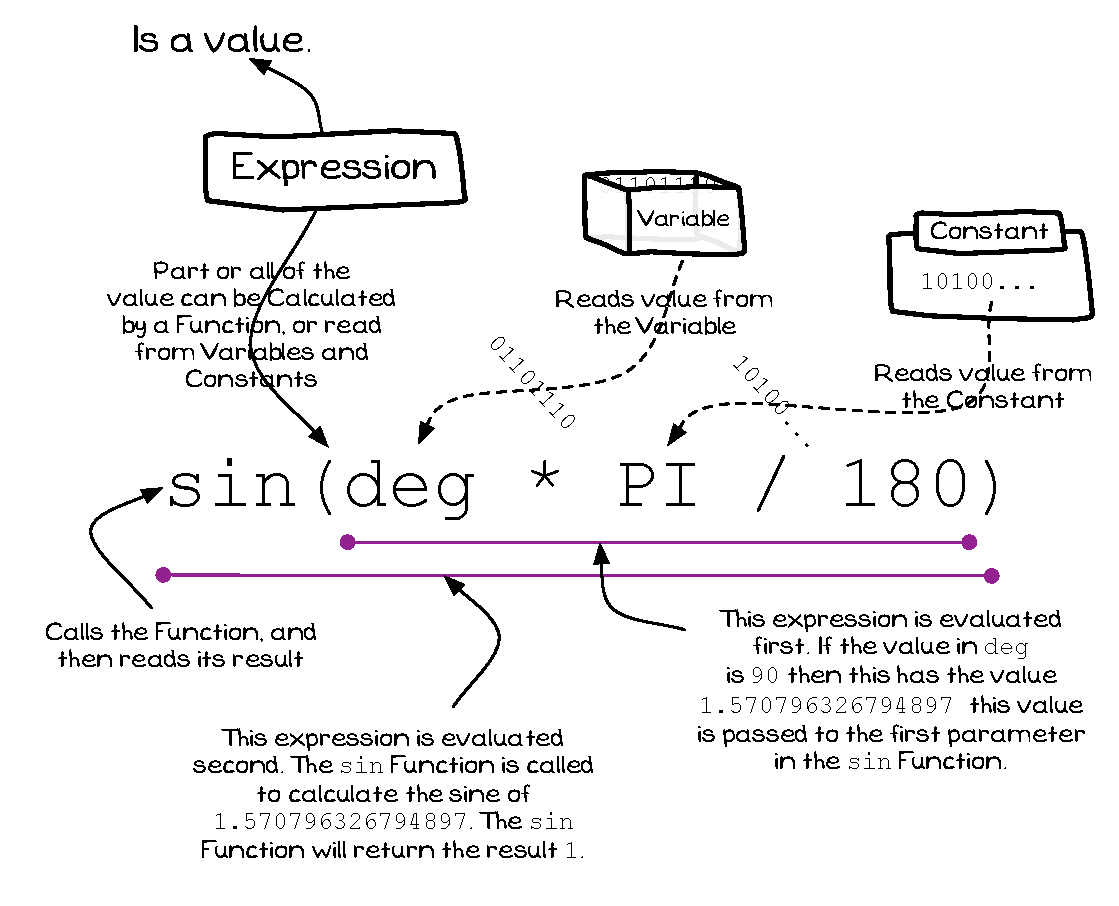
\includegraphics[width=0.9\textwidth]{./topics/storing-using-data/diagrams/Expression} 
   \caption{Expressions can read values from Function Calls, Variables, and Constants}
   \label{fig:expressions-with-variables}
\end{figure}

\mynote{
\begin{itemize}
  \item Expression is the \textbf{term} given to the code that calculates values within your Statements.
  \item You can read values from Function Calls, Variables, and Constants.
  \item You use the Variable or Constant's name to access its value within an Expression.
  \item The \nameref{sub:function_call} runs the code in the Function, and then reads the result returned.
  \item There are actually \textbf{two expressions} in Figure \ref{fig:expressions-with-variables}:
  \begin{enumerate}
    \item The first Expression is the value passed to the \texttt{sin} function (\texttt{$deg \times PI \times 180$}). This value is calculated by reading the values from the \texttt{deg} variable and the \texttt{PI} constant. These values are then used in the Expression to determine that value that is passed to the Parameter in \texttt{sin}.
    \item The second Expression is the result returned from the call to the \texttt{sin} function. This will calculate the sine of the value calculated in the first expression.
  \end{enumerate} 
  \item The Expression reads the value of the Variable \textbf{at the time} it is executed.
  \item Expressions are used to calculate values that are...
  \begin{itemize}
    \item Passed to Parameters within \nameref{sub:procedure call}s.
    \item Assigned to Variables within \nameref{sub:assignment_statement}s.
  \end{itemize}
\end{itemize}
}


% subsection expressions_with_variables_ (end)
\clearpage
\subsection{Program (with functions)} % (fold)
\label{sub:program_with_functions_}

You can declare your own Functions within the program's code.

\begin{figure}[h]
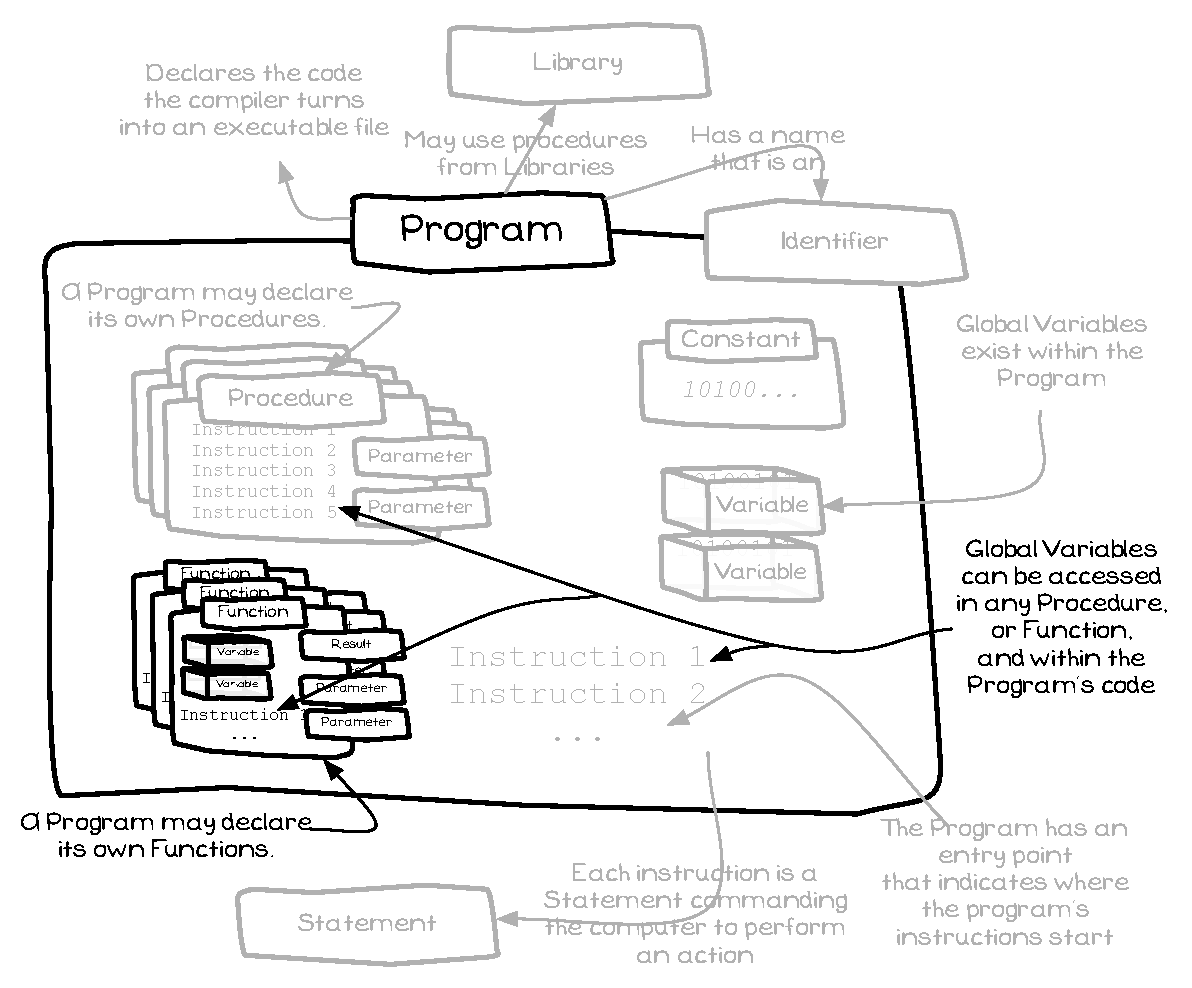
\includegraphics[width=\textwidth]{topics/storing-using-data/diagrams/ProgramWithFunctions} 
 \caption{You can declare your own Functions in your program's code}
 \label{fig:function-decl-programs}
\end{figure}

\mynote{
\begin{itemize}
  \item A Program is an \textbf{Artefact}, you create Programs that the user can execute. Internally these programs contain other artefacts such as Procedures, Functions, and Variables.
  \item You can declare your own \nameref{sub:function}s within your program's code.
  \item With C and Pascal the Function must be declared before it is used.
\end{itemize}
}

% subsection program_with_functions_ (end)

\clearpage
\subsection{Summary} % (fold)
\label{sub:data_concepts_summary}

This section has introduced a number of programming artefacts, some programming terminology, and one kind of instruction. An overview of these concepts is shown in Figure \ref{fig:data-summary}. The next section will look at how you can use these concepts to design some small programs.

\begin{figure}[h]
   \centering
   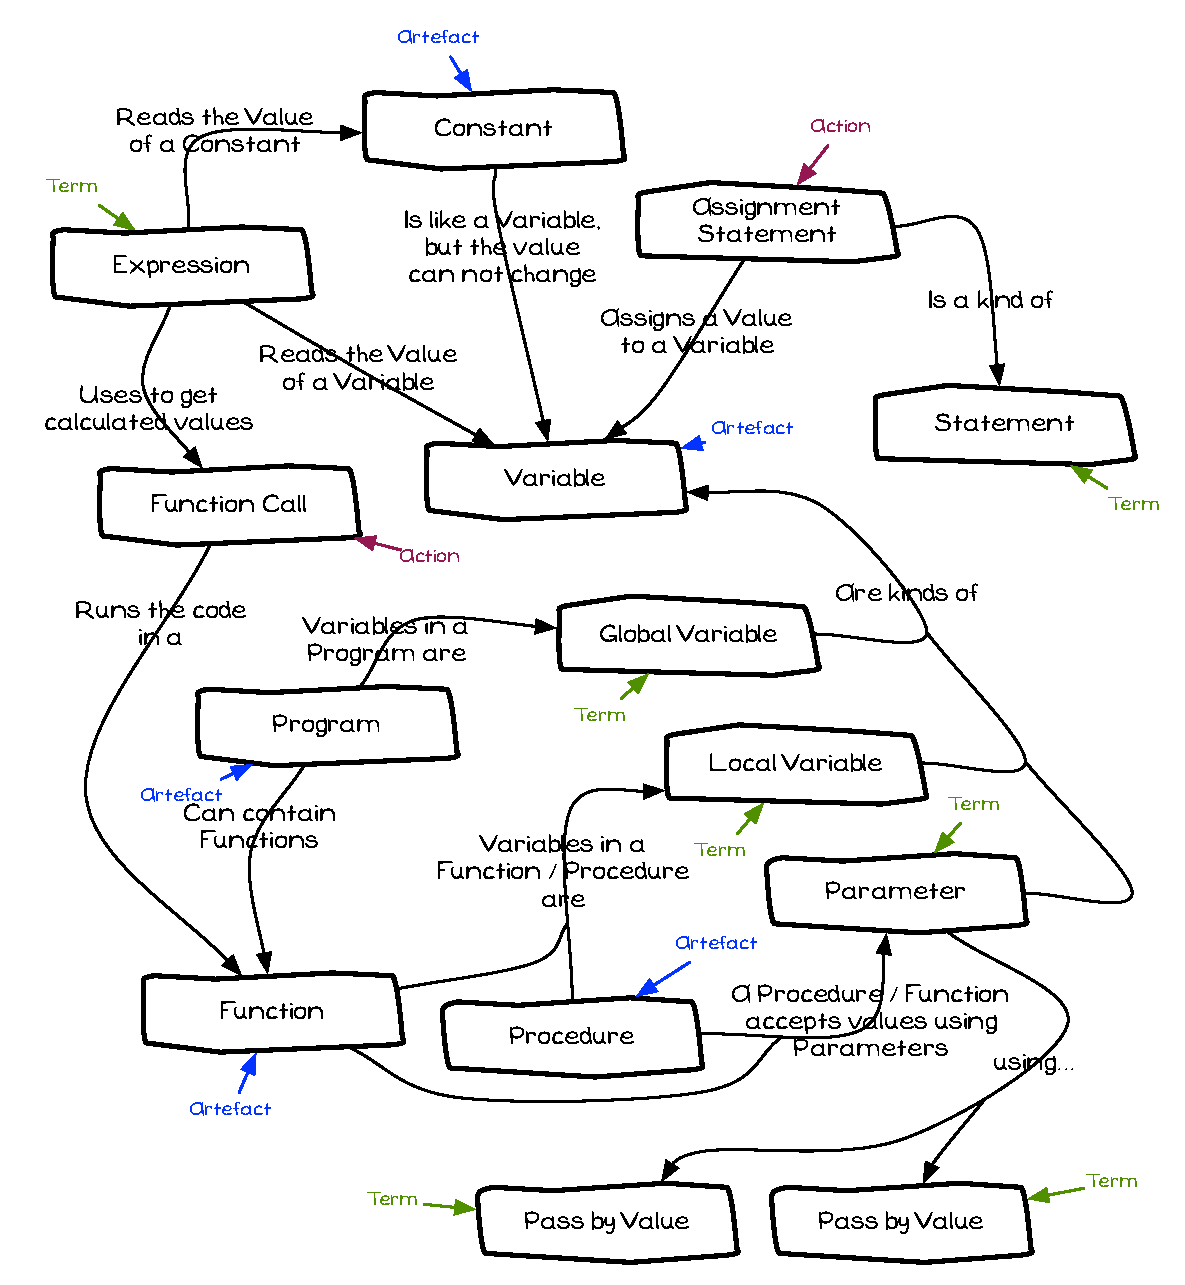
\includegraphics[width=\textwidth]{./topics/storing-using-data/diagrams/Summary} 
   \caption[Chapter Concepts]{Key Concepts introduced in this Chapter}
   \label{fig:data-summary}
\end{figure}

\mynote{
\begin{itemize}
  \item \textbf{Artefacts} are things you can \emph{create} and \emph{use}.
  \item \textbf{Terms} are things you need to \emph{understand}.
  \item \textbf{Actions} are things you can \emph{command} the computer to perform.
\end{itemize}
}

% section concepts_related_to_storing_and_using_data (end)

% ==========================================
% = Using Concepts related to data storage =
% ==========================================

\clearpage
\section{Using these Concepts} % (fold)
\label{sec:using_these_concepts_storing_using_data}

Variables, Constants, and Functions give us the ability to work with data in new ways in our programs. Previously the data within the program was limited to values entered directly into the code. Now with these concepts we can interact more meaningfully with data, performing calculations, and storing and manipulating values.

\subsection{Designing Change} % (fold)
\label{sub:designing_simple_change}

Table \ref{tbl:storing-data-prog} contains a description of the next program we are going to design. This program will calculate and output the ideal change for a given transaction from a Vending Machine. In designing this program we will make use of the concepts introduced in this chapter; we will use a Function to calculate the coins to give, Variables to store values such as the amount paid, Constants for the values of the different coins, and Parameters to pass values to the Function.

\begin{table}[h]
\centering
\begin{tabular}{l|p{10cm}}
  \hline
  \multicolumn{2}{c}{\textbf{Program Description}} \\
  \hline
  \textbf{Name} & \emph{Change Calculator} \\
  \\
  \textbf{Description} & Calculates the idea change for a given transaction in a Vending Machine. The transaction involves reading the cost of the item purchased and the amount paid, and then outputting the number of each type of coin to give as change.\\
  \hline
\end{tabular}
\caption{Description of the Change Calculator program.}
\label{tbl:storing-data-prog}
\end{table}


To design and implement this program we need to follow a number of steps:
\begin{enumerate}
  \item Understand the problem, and get some ideas on the tasks that need to be performed.
  \item Choose the artefacts we will create and use
  \item Map these artefacts to code
  \item Compile and run the program
\end{enumerate}

In step 1 you need to understand what it is that you want the program to do. This will involve determining the tasks to be performed, the steps involved in those tasks, and any data associated with them. Once you have a good understanding of what you want to achieve you can start to build a solution. In this step you determine the artefacts you want to create, and try to locate those you could use from the available libraries. Step 3 then turns your plans into source code that can be compiled and run in Step 4. 

\begin{figure}[h]
   \centering
   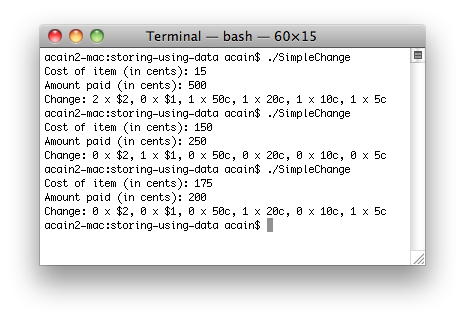
\includegraphics[width=0.4\textwidth]{./topics/storing-using-data/images/SimpleChange} 
   \caption{The Change Calculator running in the Terminal, from \fref{fig:storing-using-simeple-change}}
   \label{fig:storing-using-simeple-change-1}
\end{figure}


% subsection designing_simple_change (end)

\clearpage
\subsection{Understanding the Change Calculator} % (fold)
\label{sub:understanding_simple_change}

Receiving change from a transaction is something that you should be familiar with, and determining the ideal change is not an overly complex task. While the task itself is common, it does not mean that you can skip thinking about it. If you had to give \$6.50 in change you know without thinking that you should give three \$2 coins, and one 50c coin. What you need to do now is think through the steps that you perform intuitively.

Think about all the steps for how you actually calculated the change to be given. The first \emph{secret} is to realise that you need to start with the coin with the largest value, and then work down from there to the coin with the smallest value. The number of coins you give each time can then be calculated by dividing the amount of change to be given by the value of the current coin. Lastly you need to reduce the amount of change that remains to be given. These steps are shown in the pseudocode in Listing \ref{lst:data-simple-change-pseudo}.

\pseudocode{lst:data-simple-change-pseudo}{Pseudocode for Change Calculator program.}{./topics/storing-using-data/application/CalculateChange.txt}
% subsection understanding_simple_change (end)

\clearpage
\subsection{Choosing Artefacts for the Change Calculator} % (fold)
\label{sub:choosing_artefacts_for_simple_change}

The design for any program should involve thinking about the data as well as the tasks involved. You can start by dividing the program's tasks into functions and procedure, and then look at the data that will be needed by these in order to achieve their tasks.

\subsubsection{Designing the tasks for the Change Calculator} % (fold)
\label{ssub:designing_the_tasks_for_the_change_calculator}

Think about the process of calculating change. At the start you need to determine the amount of change that needs to be given. Next you need to determine how many of each kind of coin you are going to give. These steps can be coded into their own functions and procedures. These functions and procedures are outlined in the following list, and shown in the structure chart in \fref{fig:simple-change-structure}.

\begin{itemize}
  \item \texttt{Get Change Value}: This \nameref{sub:function} will be responsible for asking the user to enter the cost of the item, and the amount paid. It will then calculate the amount of change that needs to be given, in cents.
  \item \texttt{Give Change}: This \nameref{sub:procedure} will be responsible for the calculations related to giving one kind of coin as change. This will involve getting the number of coins to give, updating the amount of change remaining, and outputting the details (for that coin) to the Terminal.
  \item \texttt{Coins to Give}: This \nameref{sub:function} will be responsible for calculating the number of coins to give as change, given an amount of change and the value of the coin.
\end{itemize}

\begin{figure}[htbp]
   \centering
   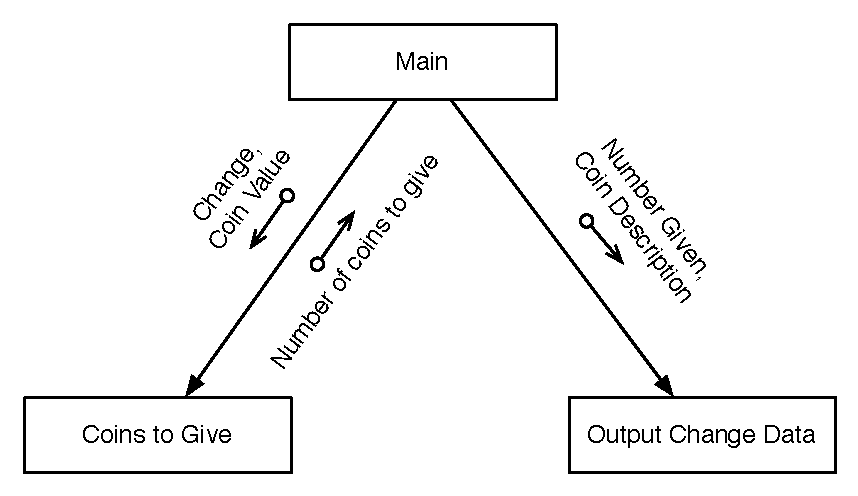
\includegraphics[width=0.6\textwidth]{./topics/storing-using-data/images/SimpleCalcStructure} 
   \caption{Structure Chart for the Change Calculator}
   \label{fig:simple-change-structure}
\end{figure}

To understand how this is going to work you now need to think about how the kinds if data these different tasks are going to need. 

% subsubsection designing_the_tasks_for_the_change_calculator (end)

\subsubsection{Designing the data for the Change Calculator} % (fold)
\label{ssub:designing_the_data_for_the_change_calculator}

Designing data is much like designing the procedures in your program. You need to think about the solution and try to identify the different values that are being used. Each of these values can then become either a Variable, a Parameter, or a Constant. Looking over the steps for calculating change you should be able to identify several different values you will need to work with. You need to be able to store things like the cost of the item being purchased, the amount of money paid, and the amount of change you need to give. A good way to approach this is to think about the values the program will output, as well as the values the user will need to input and any intermediate values you will need to perform the required calculations.

You can use the input/output/processing ideas to help you think about the data that will be required for each function or procedure. Let us examine each of the functions and procedures in turn.

\paragraph{Get Change Value} % (fold)
\label{par:get_change_value}
The first task we can examine if the \texttt{Get Change Value} \nameref{sub:function}. This task will be responsible for determining how much change needs to be given to the user. To design the data needed for this task you can think about its inputs, outputs, and temporary values.

When you are designing a function or procedure it can be given input by the calling code in the \nameref{sub:function_call} or \nameref{sub:procedure call}. Inputs provided via the function or procedure call are coded using \nameref{sub:parameter}s. To determine the parameters you need, think about the information that this function or procedure will need to be given to fulfil its responsibilities. In the case of the \texttt{Get Change Value}, it does not require any input from the caller.

\begin{itemize}
  \item \texttt{Get Change Value} does not require any input from the calling code, so there is no need for any parameters with this function.
\end{itemize}

The \texttt{Get Change Value} task will be coded as a function because it has some output. The result returned by a function is an output, it is what makes it different from a procedure. When you call a function it runs some steps and then returns a value, the value returned is the output from the function. \texttt{Get Change Value} needs to return back the amount of change, this is why it is a function in this design.

\begin{itemize}
  \item \texttt{Get Change Value} returns a number. The number returned is the value of the change to be given in cents.
\end{itemize}

Within the \texttt{Get Change Value} function there will need to be some values that it uses to calculate its output. \texttt{Get Change Value} will need to read the cost of the item from the user, and the amount paid. These two values need to be stored somewhere, so the design of this function will require two \nameref{sub:local_variable}s: they can be called \texttt{Cost of Item} and \texttt{Payment}. These will exist entirely within the function, being the values the function requires to calculate its output.

\begin{itemize}
  \item \texttt{Get Change Value} will have two local variables: \texttt{Cost of Item} and \texttt{Payment}.
\end{itemize}

The pseudocode for this function is shown in \lref{lst:get_change_value}.

\pseudocode{lst:get_change_value}{Pseudocode for the \texttt{Get Change Value} function}{./topics/storing-using-data/application/GetChangeValue.txt}

% paragraph get_change_value (end)

\paragraph{Give Change} % (fold)
\label{par:give_change}
The next task to consider is the \texttt{Give Change} \nameref{sub:procedure}. This procedure will be responsible for coordinating the actions for giving a certain coin in change. Once again you need to think about the inputs it requires (parameters), its outputs, and any values it will work with internally.

Put yourself in the place of the computer.\footnote{Remember the computer is unintelligent. You cannot rely upon your knowledge. Try to think about the information you are using and the steps you are performing to make sure you can capture what needs to be done in your code.} You (as the computer) have been \emph{asked} to \texttt{Give Change}. What data will you need to complete this request? At a minimum you will need to know the total change value that is being given, and the value of the coin that you are issuing.\footnote{In this design the \texttt{Give Change} procedure will be called once for each coin.}

There is one more input that you can only find by thinking about the tasks the computer needs to perform in this code. A part of giving the change will be to output a message, something like `3 x 20c' or `1 x \$2'. The number of coins can be calculated within the procedure, but the text is another issue. The computer will not know what text to output. This data must, therefore, come as input into the procedure.

\begin{itemize}
  \item \texttt{Give Change} needs to be \emph{given} the \texttt{Change Value} variable, and it needs to be told value of the coin and the coin's description. These will be coded as parameters, with \texttt{Change Value} being passed by reference.
\end{itemize}

\texttt{Give Change} will output text to the Terminal, but it also needs to update the \texttt{Change Value} variable it is given. This can be considered as output from the procedure. As the \texttt{Change Value} variable is passed by reference, you can picture this as receiving the variable from the caller. Any changes this procedure makes on its \texttt{Change Value} parameter will actually be changing the value in the variable passed to the \texttt{Give Change} procedure. In this way the procedure is able to output a value.\footnote{An alternative implementation could have been to code this as a \nameref{sub:function}, with the new change value being returned. It would then be the responsibility of the caller to assign this into their change variable.}

\begin{itemize}
  \item \texttt{Give Change} will output the updated \texttt{Change Value}, as this is passed by reference.
\end{itemize}

Within \texttt{Give Change} you will need to store the number of coins to give in change. This will become a local variable that can be used to calculate the updated \texttt{Change Value} and to output the details to the Terminal.

\begin{itemize}
  \item \texttt{Give Change} will have one local variable: \texttt{to give} used to store the number of this coin to be given in the change.
\end{itemize}


The pseudocode for this procedure is shown in \lref{lst:give_change}.

\pseudocode{lst:give_change}{Pseudocode for the \texttt{Give Change} function}{./topics/storing-using-data/application/GiveChange.txt}

% paragraph give_change (end)

\paragraph{Coins to Give} % (fold)
\label{par:coins_to_give}
The \texttt{Coins to Give} function is used to calculate the number of coins to give. This code could have been written within the \texttt{Give Change} procedure, but it was decided to code this in its own function. 

\texttt{Coins to Give} will need to be told the value of the change, and the value of the coin. Both of these parameters will be passed by value, as it is only the values that are required. Internally \texttt{Coins to Give} will not require any additional data, as it can calculate its output from the two input values.

\begin{itemize}
  \item \texttt{Coins to Give} needs to be \emph{told} the value of the change and the value of the coin, it can then use these values to calculate the number of these coins that need to be given in the change.
  \item \texttt{Coins to Give} will output the number of the indicated coin that needs to be given in the change.
\end{itemize}


The pseudocode for this procedure is shown in \lref{lst:coins_to_give}.

\pseudocode{lst:coins_to_give}{Pseudocode for the \texttt{Coins to Give} function}{./topics/storing-using-data/application/CoinsToGive.txt}

% paragraph coins_to_give (end)

\paragraph{Entry Point (Main)} % (fold)
\label{par:entry_point_main_}
The program's code always performs the same task. It coordinates the actions the program is performing. The pseudocode for this was shown in \lref{lst:data-simple-change-pseudo}. This code will need to store the value of the change. It will get the value to store in this by calling \texttt{Get Change Value}. It will call \texttt{Give Change} for each of the coin values, and pass this variable to the procedure for it to update. These actions are shown in \fref{fig:simple-change-seq}.

\begin{itemize}
  \item The \texttt{Entry Point (Main)} needs a local variable to store the \texttt{Change Value}.
\end{itemize}

Thinking further about the program there are also the constant values of the different coins. These values are almost taken for granted when you think about giving change yourself, but remember the computer is unintelligent so you need to specify \emph{everything} for it. The values of the coins can be coded using a constant for each coin. Using constants is a better option than hard coding these values directly in the program, as the name helps provide a context for the value when it is used.

\mynote{
\begin{itemize}
  \item Notice that the functions and procedures are isolated from each other. They have defined inputs and outputs, but their local variables are hidden within their code.
  \item This means you can focus on the function/procedure you are working on, and do not have to think much about the details of the other functions/procedures in your code.
  \item Parameters allow you to pass data into a function/procedure.
  % \item A function returns a value to the caller.
  \item Passing a parameter by reference allows you to output a value by updating the variable you are passed. This means a procedure can output values by having parameters passed by reference, and functions can also use this mechanism to update values in variables as well.
\end{itemize}
}

\begin{figure}[htbp]
   \centering
   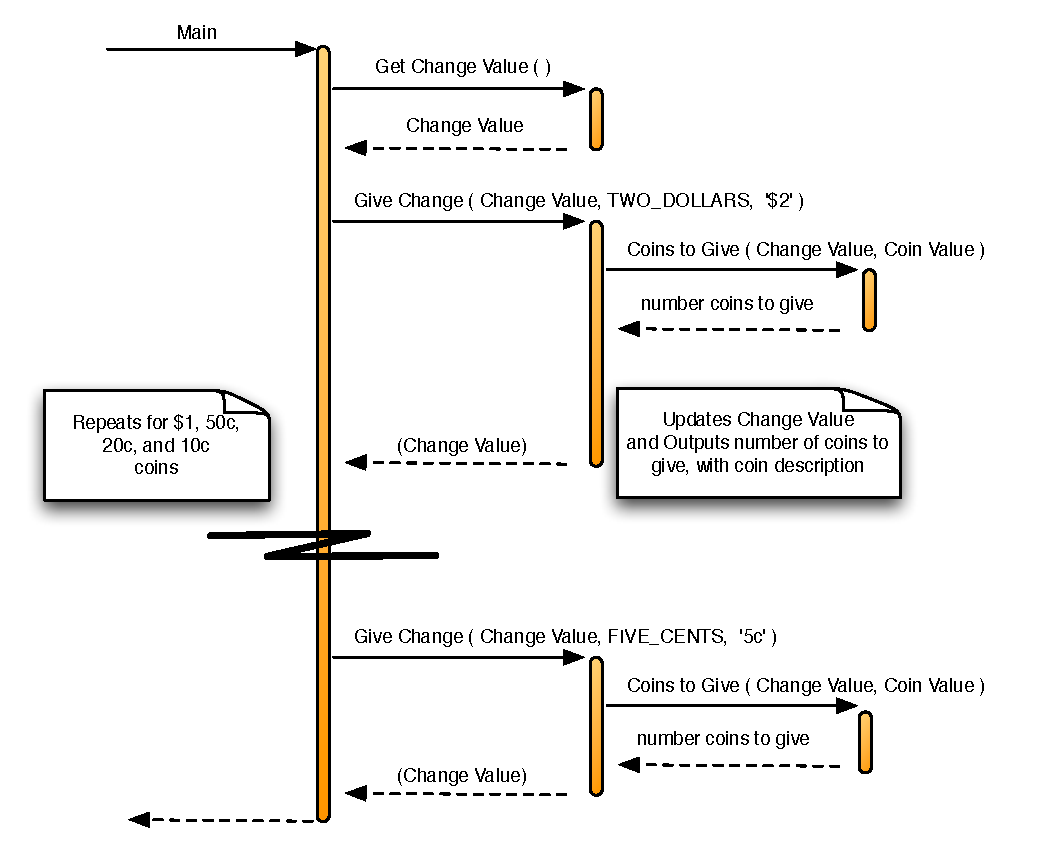
\includegraphics[width=\textwidth]{./topics/storing-using-data/images/SimpleCalcSeq} 
   \caption{Sequence Diagram for the Change Calculator}
   \label{fig:simple-change-seq}
\end{figure}

\clearpage
% paragraph entry_point_main_ (end)
% subsubsection designing_the_data_for_the_change_calculator (end)

\subsubsection{Change Calculator Design Overview} % (fold)
\label{ssub:change_calculator_design_overview}

The Change Calculator program contains the following artefacts:

\begin{itemize}
  \item \textbf{Constants}:
  \begin{itemize}
    \item \texttt{\textbf{TWO\_DOLLARS}} with value 200, represents the value of a \$2 coin
    \item \texttt{\textbf{ONE\_DOLLAR}} with value 100, represents the value of a \$1 coin
    \item \texttt{\textbf{FIFTY\_CENTS}} with value 50, represents the value of a 50c coin
    \item \texttt{\textbf{TWENTY\_CENTS}} with value 20, represents the value of a 20c coin
    \item \texttt{\textbf{TEN\_CENTS}} with value 10, represents the value of a 10c coin
    \item \texttt{\textbf{FIVE\_CENTS}} with value 5, represents the value of a 5c coin
  \end{itemize}
  \item \textbf{Functions}:
  \begin{itemize}
    \item \texttt{\textbf{Get Change Value}}: Calculates and returns the amount of change that needs to be given by the program. This function has the following:
    \begin{itemize}
      \item  \textbf{Local Varaibles}:
      \begin{itemize}
        \item \textbf{\texttt{Cost of Item}}: Stores the value of the item being purchased. This design uses cents as its base to make the calculations easier, avoiding rounding issues involved in using floating point values.
        \item \texttt{\textbf{Payment}}: This is used to store the value of the payment being made. Once again this will be in cents.
      \end{itemize}
    \end{itemize}
    \item \texttt{\textbf{Coins to Give}}: Calculates the number of coins to give, returning how many of these coins should be dispensed as part of giving this change. This has the following:
    \begin{itemize}
      \item  \textbf{Parameters}:
      \begin{itemize}
        \item \texttt{\textbf{Change}}: The value of the change that is to be given.
        \item \texttt{\textbf{Coin Value}}: The value of the coin that is being dispensed.
      \end{itemize}
    \end{itemize}
  \end{itemize}
  \item \textbf{Procedures}:
  \begin{itemize}
    \item \texttt{\textbf{Give Change}}: Calculates the change, and outputs the coin details to the Terminal. This shows the number and description of the change given. This requires the following:
    \begin{itemize}
      \item \textbf{Parameters}:
      \begin{itemize}
        \item \textbf{\texttt{Change Value}} (by reference): The variable that is storing the amount of change to be given.
        \item \textbf{\texttt{Coin Value}}: The value of the coin to issue.
        \item \textbf{\texttt{Coin Description}}: The description of the coin.
      \end{itemize}
      \item \textbf{Local Variables}:
      \begin{itemize}
        \item \texttt{\textbf{To Give}}: Stores the number of the coin to give in change, used to update the \texttt{Change Value} and to output the message.
      \end{itemize}
    \end{itemize}
    \item \textbf{\texttt{Entry Point (Main)}}: this coordinates the overall activity of the program. Getting the amount of change using \texttt{Get Change Value}, and using \texttt{Give Change} to issue the change for each coin.
    \begin{itemize}
      \item \textbf{Variables}:
      \begin{itemize}
        \item \texttt{\textbf{Change Value}}: Keeps track of the current amount of change that has to be given to the user.
      \end{itemize}

    \end{itemize}
  \end{itemize}  
\end{itemize}

In addition to these artefacts the program will make use of some procedures from the available libraries. This will include the following:
\begin{itemize}
  \item \textbf{Output}: You need to use your language's procedures to write output to the Terminal.
  \item \textbf{Input}: Languages also provide a means of reading values from the user. In C and Pascal these input procedures need to be passed the variables that you want the value assigned to. This uses pass by reference to enable the input procedure to store the values read into a variable for you.
\end{itemize}

\csection{
In C the input procedure to read values from the Terminal is called \csnipet{scanf()}, see \nameref{sub:c_terminal_input}.
}

\passection{
In Pascal the input procedure to read values from the Terminal is called \passnipet{ReadLn()}
, see \nameref{sub:pas_terminal_input}.}

% subsubsection change_calculator_design_overview (end)

\subsubsection{Reviewing the design diagrams} % (fold)
\label{ssub:reviewing_the_design_diagrams}

Figure \ref{fig:simple-change-structure} shows the Structure Chart for the Change Calculator. This shows the structure of the solution, visually showing the functions and procedures and the calls between them. This diagram has been enhanced to show the parameter values being passed into the functions and procedures, and the values being returned. These data flows are shown alongside the call arrow, with their own smaller arrow to indicate the direction of the flow. 

By reading \fref{fig:simple-change-structure} you can tell that \texttt{Coins to Give} is going to be a function as it is returning data to \texttt{Main}. \texttt{Give Change} could be a function or a procedure as it is accepting and returning the \texttt{Change Value}, in this design it is a procedure, and updates the value in the \texttt{Change Value} variable using pass by reference. You can also see that \texttt{Coins to Give} and \texttt{Give Change} both require parameters to accept the data being passed into them. 

The Structure Chart shows the static structure of the code, indicating the calls between the functions and procedures, but not communicating when these are called, or how many times. This dynamic information is captured in the Sequence Diagram shown in Figure \ref{fig:simple-change-seq}. This diagram shows the sequence in which the function and procedure calls are performed. Notice that this diagram has also been enhanced to show the data that flows into and out of the functions and procedures. 

The Sequence Diagram indicates how values are being returned. The return of a function's value is shown by indicating the value on the returning arrow. Notice the indication of this value on the arrow returning from the call to \texttt{Get Change Value}, this indicates that \texttt{Get Change Value} is a function. On the other hand, the brackets around the return value from \texttt{Give Change} indicates that this is being performed by updating a parameter that was passed using pass by reference. You can use this information to determine how the design intends these to be coded. As \texttt{Get Change Value} is directly returning a value it must be a function, \texttt{Give Change} updates a parameter and does not return a value itself so it must be a procedure.

\mynote{
\begin{itemize}
  \item A structure chart shows the static structure of the program. This tells you which procedure/functions call which, and the data that is passed between them. It shows you what is written in the code.
  \item A sequence diagram shows the dynamic operation of a program. This tells you how the functions and procedures interact to achieve some goal. It shows you what is happening when the code is run.
\end{itemize}
} 

% subsubsection reviewing_the_design_diagrams (end)

\clearpage
\subsubsection{Designing data in general} % (fold)
\label{ssub:designing_data_in_genera}

When you are designing a program you need to think about each function or procedure, and determine if it requires data to be given to it to enable it to perform its action. Any data it requires must then be passed to it using Parameters. The key to understanding parameters is to remember that each function/procedure is its own isolated domain. It can have its own data, using local variables, and has its own instructions. In most cases these instructions will need to be given some starting data, some information upon which to act. 

One strategy you can use to picture this is to put yourself in the place of the function, or procedure. For example, what would you need to be told in order to determine the number of coins to give in change for a single coin type. You can not work out the answer without being told the value of the change to be given, and the value of the coin. With these two pieces of information you now have enough to calculate the required output. For example, how many \$2 coins should be given for \$6.50 in change. These two pieces of data can be used to calculate the answer 3. This is exactly what is being coded in the \texttt{Coins to Give} function.

In this respect Procedures are the same. In order to give change, the \texttt{Give Change} procedure needs some information. It can not act without this information. If you needed to \emph{give change}, you need to be told something about the amount of change you are giving and the value of the coin you are issuing. In this case, \texttt{Give Change} needs to be told the \texttt{change value}, the \texttt{coin value}, and the description of that coin. With these details the procedure can then code the steps needed to produce its desired side effects.

Parameters are mostly used to pass a value into a function or procedure. However, in some cases it is useful to pass in the \emph{variable} rather than the \emph{value}. This is the case when you want the function or procedure to \emph{change} the value in the variable passed to it. Take the \texttt{change value} parameter in \texttt{Give Change} as an example. When this procedure issues some coins, the amount of change still to be given must be updated. For example, when you issue `3 x \$2' for the \$6.50 in change, the new change value will be 50c ($650 - (3 \times 200)$). By passing the \emph{variable} into \texttt{Give Change} it is possible for this code to change the value in the callers variable, ensuring that the correct change is given.

% subsubsection designing_data_in_genera (end)

\subsubsection{Modelling and Abstraction} % (fold)
\label{ssub:modelling_and_abstraction}

One of the main keys to understanding programs, and to creating good designs, is to see how each artefact you create models something from the problem. The procedures that you create model the processes, performing actions that relate to the task at hand. The functions model calculations that need to be performed, such as determining how many coins should be given. In the same way the variables that you create will store values related to the problem. Each variable \textbf{represents} something, some information related to your program. The \emph{thing} it represents should be reflected in the name given to the variable.

The act of trying to model the problem in software is called \textbf{abstraction}. It is the process of determining the features of the problem that are essential to the solution, and capturing these in a way that models reality but keeps only the details we care about. The ability to create your own model is a skill that you learn with experience, taking a lot of practice to really master.

\mynote{
\begin{itemize}
  \item A good design will closely model the program's domain. You should be able to relate the artefacts you are creating with things related to the program.
\end{itemize}
}

% subsubsection subsubsection_name (end)
% subsection choosing_artefacts_for_simple_change (end)

\clearpage
\subsection{Writing the Code for the Change Calculator} % (fold)
\label{sub:writing_the_code_for_simple_change}

The pseudocode from Listing \ref{lst:data-simple-change-pseudo} shows the instructions, and how these should be divided between the \texttt{Coins to Give} Function and \texttt{Output Change Data} Procedure. At this stage these instructions need to be translated into source code, so that they can be compiled and the resulting program tested.

The following two sections, Section \ref{sec:storing_and_using_data_in_c} \nameref{sec:storing_and_using_data_in_c} and Section \ref{sec:storing_and_using_data_in_pascal} \nameref{sec:storing_and_using_data_in_pascal}, contain a description of the syntax needed to create programs in the C and Pascal programming languages that include Variable and Function declarations.

\mynote{
Remember the basic process for reading the Syntax Diagrams is to:
\begin{enumerate}
  \item Find the page with the Syntax rule you are interested in knowing about.
  \item Have a quick look at the Syntax Diagram and the rules it contains. Read each rule, and get a basic feel for how it is going to come together for your program.
  \item Read the example to see one way of using the Rule. The Syntax Diagram can be used to create any number of variations of the rule, the example gives you at least one way these rules can be coded.
  \item Return to the diagram and make sure you can match each part of the example back to the rule that created it.
  \item Look up any related rules that are not explained on this rule's page.
\end{enumerate}
}
% subsection writing_the_code_for_simple_change (end)

\clearpage
\subsection{Compiling and Running the Change Calculator} % (fold)
\label{sub:compiling_and_running_simple_change}

Once you have completed your program, you need to compile and test it. 

\begin{enumerate}
  \item Open the \textbf{Terminal}\footnote{The \textbf{MinGW Shell} on Windows.} program for your Operating System
  \item Use the \texttt{\textbf{cd}} command to move to the directory with your code, for example \newline \bashsnipet{cd /Users/acain/Documents/Code}
  \item Run the compiler with your program's code. See the language specific details below.
  \item Fix any compiler errors, using the tips from Section \ref{ssub:compiler_errors} \nameref{ssub:compiler_errors}.
  \item Execute the program using \bashsnipet{./SimpleChange} and check the results
\end{enumerate}

\csection{
The C compiler is called \textbf{gcc}. To compile your \emph{Change Calculator} program you will need to run the following: \newline \newline \bashsnipet{gcc -o SimpleChange simple-change.c}
}

\cppsection{
C does not have support for pass by reference, though it can be achieved using other means (see \cref{cha:dynamic_memory_allocation}). The C++ language is an extension to C that fixed a number of issues, as well as added some new features. One of the new features was built in pass by reference. To compile the C++ version of the Change Calculator you need to use the C++ compiler called \textbf{g++}. To compile your \emph{Change Calculator} program you will need to run the following: \newline \newline \bashsnipet{g++ -o SimpleChange simple-change.cpp}
}

\passection{
The Pascal compiler is called \textbf{fpc}. To compile your \emph{Change Calculator} program you will need to run the following: \newline \newline \bashsnipet{fpc -S2 SimpleChange.pas}
}

\clearpage
\subsubsection{Generating Test Data} % (fold)
\label{ssub:generating_test_data}

Now that our program is making greater use of data it becomes more important to think about how to test your program. Testing is the process of trying to locate issues with your code. There are two main classifications for issues, \textbf{syntactic errors} and \textbf{semantic errors}.

Syntactic errors indicate places in your code where you have not correctly followed the syntax of the language. These are the easiest kind of error to find as the compiler will not be able to compile the program if its syntax is not correct. The errors that the compiler report are all syntax errors. As you gain experience with a Language you will find that you make fewer and fewer of these kinds of errors. 

Semantic errors, on the other hand, will not be found by the compiler. These are errors in the logic within the program. They are cases where you have correctly structured the code, but the code itself does not get the computer to perform the actions you require. These are the kinds of errors that you need to learn to be able to detect yourself. Selecting the right kind of test data is an important task when you start to think about testing programs.

For the Change Calculator there are two inputs provided by the user. In order to test this program you need to determine the values that are passed to the \texttt{Cost of the Item} and the \texttt{Payment} inputs. You want to choose values that can help you uncover any unexpected issues with the programs code.

\begin{table}[htbp]
\begin{tabular}{|l|l|l|p{7cm}|}
  \hline
  \textbf{Cost of Item}  & \textbf{Payment} & \textbf{Expected Output}  &   \textbf{Reason} \\
  \hline
  \$2.50 & \$5.00 & 1 x \$2, 1 x 50c & Basic test to check that the program works for a simple data input. \\
  \hline
  \$0.15 & \$4.00 & 1 of each coin & Generates \$3.85 in change, checking that each coin is used. \\
  \hline
  \$0.05 & \$0.10 & 1 x 5c & Check the output can be a single coin. Could also add tests to check other individual coins. \\
  \hline
  \$0.60 & \$1.00 & 2 x 20c & Check that 2 coins can be given. \\
  \hline
  \$0.00 & \$5.00 & 2 x \$2, 1 x \$1 & Can it accept no cost of item, and give back payment? \\
  \hline
  \$3.85 & \$0.00 & -1 of each coin & Check what happens if insufficient funds are provided. \\
  \hline
\end{tabular}
\caption{Test Data for the Change Calculator}
\label{tab:simple_change_test_data}
\end{table}

The data we use to test an execution of a program is called a \textbf{Test Case}. Each test case provides a set of input values, and the expected results given this input. Example test cases for the Change Calculator are shown in Table \ref{tab:simple_change_test_data}. This table shows the input values, the expected output values, and some rational for why this test case should be run. To perform the testing you run the program once for each test case and check the output of the program against the expected output. If there are any differences you know that their is a problem, and need to check the program's code to find the source of the logic errors.




% subsubsection generating_test_data (end)

% subsection compiling_and_running_simple_change (end)


% section using_these_concepts (end)


% ===============================
% = Storing and Using Data in C =
% ===============================

\clearpage
\def\pageLang{c}
\section{Storing and Using Data in C} % (fold)
\label{sec:storing_and_using_data_in_c}

\subsection{Implementing Simple Change in C} % (fold)
\label{sub:implementing_simple_change_in_c}

Section \ref{sec:using_these_concepts_storing_using_data} of this chapter introduced the `Simple Change Calculator' program, and its design. Its implementation requires the definition of a Function as well as a Procedure in the Program's code. The Procedure and Function accepted parameters, and the Program's code uses Local Variables. This section of the chapter introduces the C syntax rules for implementing these concepts using the C language. The C implementation of the Simple Change Calculator are shown in Listing \ref{lst:storing-data-c-simple-change}.

\straightcode{\ccode{lst:storing-data-c-simple-change}{C code for the Simple Change Calculator}{code/c/storing-using-data/simple-change.c}}

\mynote{
\begin{itemize}
  \item Save the C code in a file named \texttt{simple-change.c}.
  \item Compile this using \bashsnipet{gcc -o SimpleChange simple-change.c}.
  \item Run the resulting program using \bashsnipet{./SimpleChange}.
  \item Perform each of the Test Cases from Table \ref{tab:simple_change_test_data} and check that the output matches the expected values.
  \item Look over the code and examine how the Variables, Parameters, Constants, and Function are being used.
  \item Notice how the indentation makes it easy to see where each Function and Procedure starts and ends. Always lay your code out so that it is easy to see its structure.
  \item See how the Function and Procedure are declared before they are used. This is important as the C compiler reads the code from the start, and must know about the artefacts before you use them.
\end{itemize}
}



% subsection implementing_simple_change_in_c (end)
\clearpage
\subsection{C Variable Declaration} % (fold)
\label{sub:c_variable_declaration}

A Variable Declaration allows you to create a Variable in your Code. In C you can declare variables in the program's code, and in Functions and Procedures. 

\csyntax{csynt:storing-using-data-variable-decl}{Variable Declaration}{storing-using-data/variable-declaration}

\csection{\ccode{lst:variable-test-c}{Variable Declaration Tests}{code/c/storing-using-data/variable_test.c}}

\mynote{
\begin{itemize}
  \item This is the C Syntax for creating your own \nameref{sub:variable}.
  \item This syntax can be used to declare \ldots
  \begin{itemize}
    \item Local Variables within Functions and Procedures.
    \item Global Variables within the program.
  \end{itemize} 
  \item In C the Variable Declaration starts with the \nameref{sub:type} name indicating the kind of data that will be stored.
  \item Following the Type is a list of the identifiers for the Variables that are being created. You can create one or more variables in a single Variable Declaration, but all of these Variables will have the same type.
  \item Each variable can be assigned a value when it is declared.
  \item The \textbf{const} modifier can be added to the start of a Variable declaration to create a Constant.
  \item See \nameref{sub:c_procedure_declaration_with_local_variables_} for details on declaring Local Variables within Functions and Procedures.
  \item See \nameref{sub:c_program_with_global_variables} for details on declaring Global Variables within the program itself.
  \item The syntax for declaring Parameters is very similar, see \nameref{sub:c_procedure_declaration_with_parameters_}.
\end{itemize}
}

% subsection c_variable_declaration (end)
\clearpage
\subsection{C Program (with Global Variables and Constants)} % (fold)
\label{sub:c_program_with_global_variables}

You can declare Global Variables and Constants within a C Program file.

\csyntax{csynt:storing-using-data-program}{a Program (with global variables and constants)}{storing-using-data/program-with-globals}

\mynote{
\begin{itemize}
  \item This syntax allows you to declare \nameref{sub:global_variable}s and Constants.
  \item See Listing \ref{lst:variable-test-c} for an example of declaring Global Variable and Constants.
  \item In Listing \ref{lst:variable-test-c} \ldots
  \begin{itemize}
    \item \texttt{global\_float} and \texttt{global\_int} are Global Variables. These can be accessed in both the \texttt{test} procedure and \texttt{main}.
    \item \texttt{PI} is a Global Constant, with the value 3.1415. This can be read in both the \texttt{test} procedure and \texttt{main}.
  \end{itemize}
  \item Global variable should be avoided.
  \item There are a number of conventions, called coding standards, that describe how your code should appear for a given language. In this text we will use a common C convention of having all \emph{Constants} in \textbf{UPPER CASE}, with underscores ( \_ ) used to separate words. So the \emph{Maximum Height} constant becomes \texttt{MAXIMUM\_HEIGHT}.
\end{itemize}
}

% subsection c_program_with_global_variables (end)
\clearpage
\subsection{C Procedure Declaration (with Local Variables)} % (fold)
\label{sub:c_procedure_declaration_with_local_variables_}

The Functions and Procedures in C can contain declaration for \nameref{sub:local_variable}s.

\csyntax{csynt:storing-using-data-procedure-decl}{Procedure Declaration (with Local Variables)}{storing-using-data/procedure-decl-with-locals}

\mynote{
\begin{itemize}
  \item This is the syntax for declaring \nameref{sub:local_variable}s in a Procedure.
  \item See Listing \ref{lst:variable-test-c} for an example of declaring Local Variables.
  \item In Listing \ref{lst:variable-test-c} \ldots
  \begin{itemize}
    \item The \texttt{test} procedure has two local variables: \texttt{my\_local} and \texttt{another\_local}.
    \item The \texttt{main} function has one local variable called \texttt{local\_int}.
  \end{itemize}
  \item The Local Variables must be declared before the statements within the Function and Procedure's block.
  \item In C you cannot declare variables after the first statement in the block.
  \item In this text we will use a common C convention of having all \emph{Local Variables} in \textbf{lower case}, with underscores ( \_ ) used to separate words. So the \emph{My Name} local variable becomes \texttt{my\_name}.
  
\end{itemize}
}

% subsection c_procedure_declaration_with_local_variables_ (end)
% \clearpage
\subsection{C Statement (with the Assignment Statement)} % (fold)
\label{sub:c_statement_with_assignment}

\csyntax{csynt:storing-using-data-statement}{Statement (with the Assignment Statement)}{storing-using-data/statement-with-assignment}

% subsection c_statement_with_assignment (end)
\clearpage
\subsection{C++ Assignment Statement} % (fold)
\label{sub:c_assignment_statement}

The assignment statement is used to store a value in a variable.

\csyntax{csynt:storing-using-data-assignment-statement}{an Assignment Statement}{storing-using-data/assignment-statement}

\mynote{
\begin{itemize}
  \item This is the C++ syntax for the \nameref{sub:assignment_statement}.
  \item In C++ assignment is indicated by the equals sign ( = ).
  \item The \emph{left hand side} of the assignment must be a valid variable, this is where the value is to be stored.
  \item The \emph{right hand side} of the assignment is an expression, this calculates the value that will be stored in the Variable.
  \item There are multiple versions of the assignment, giving short hand ways of using the current value.
  \begin{itemize}
    \item \textbf{\texttt{=}} is the standard assignment, this stores the value of the expression in the Variable.
    \item \textbf{\texttt{+=}} increments the variable's value, \newline \csnipet{a += n;} is equivalent to \csnipet{a = a + n;}
    \item \textbf{\texttt{-=}} decrements the variable's value, \newline \csnipet{a -= n;} is equivalent to \csnipet{a = a - n;}
    \item \textbf{\texttt{*=}} multiplies the value in the variable by a given factor. \newline \csnipet{a *= n;} is equivalent to \csnipet{a = a * n;}
    \item \textbf{\texttt{/=}} divides the value in the variable by a factor. \newline \csnipet{a /= n;} is equivalent to \csnipet{a = a / n;}
  \end{itemize}
  \item The \texttt{++} and \texttt{-{-}} operators allow a variables value to be increments or decremented.
\end{itemize}
}

\csection{\ccode{lst:assignment-test-c}{Assignment Tests}{code/c/storing-using-data/assignment-test.c}}


% subsection c_assignment_statement (end)
\clearpage
\subsection{C Procedure Declaration (with Parameters)} % (fold)
\label{sub:c_procedure_declaration_with_parameters_}

In C \nameref{sub:parameter}s can be declared in any Function or Procedure declaration.

\csyntax{csynt:parameter-procedure-decl}{Procedure Declarations (with Parameters)}{parameters/procedure-decl-with-params}

\mynote{
\begin{itemize}
  \item The syntax in Figure \ref{csynt:parameter-procedure-decl} shows the C code for declaring Procedures with \nameref{sub:parameter}s.
  \item Parameters in C are declared in a similar way to other Variables, with the \nameref{sub:type} name appearing first followed by the Parameter's name.
\end{itemize}
}

\csection{\ccode{lst:parameter-test-c}{Assignment Tests}{code/c/storing-using-data/parameter-test.c}}

% subsection c_procedure_declaration_with_parameters_ (end)
\clearpage
\subsubsection{C++ Reference Parameters} % (fold)
\label{ssub:c_reference_parameters}

C has limited support for pass by reference, but this feature was added with the extensions in the C++ language. The following syntax shows how to declare a parameter that will be passed by reference. Please note that this is not standard C code, and will require you to use a C++ compiler.

\cppsyntax{csynt:by-ref-parameter}{by-ref Parameters}{parameters/cpp-fn-decl-with-by-ref}

\cppsection{\ccode{clst:doubleif}{Example of passing by reference using C++}{code/c/storing-using-data/test-byref.cpp}}


\mynote{
\begin{itemize}
  \item This requires a \textbf{C++ compiler}, such as the \texttt{g++} compiler.
  \item C++ to an extension of the C compiler, so your C code should be able to be compiled with the C++ compiler.
  \item The C++ compiler is more strict on some rules than the C compiler. This means the compiler will give you more help in avoiding some poor programming practices.
  \item Notice that with pass by reference you do not need to do anything special in the call, the compiler takes care of the necessary details needed to achieve this.
\end{itemize}
}

% subsubsection c_reference_parameters (end)
\clearpage
\subsection{C Procedure Call (with pass by reference)} % (fold)
\label{sub:c_procedure_call_with_pass_by_reference}

Many languages support pass by reference in the compiler. This is where the compiler manages the passing of the reference for you in the background. Unfortunately C does not do this transparently and you need to manually pass the reference yourself. Its good to know that the concept remains the same, but it does mean that you must manually add code to achieve this.

\csyntax{csynt:parameter-procedure-call}{Procedure Call (with pass by reference)}{parameters/procedure-call-with-ref}

\mynote{
\begin{itemize}
  \item With C you must manually pass parameters by reference using the ampersand (\texttt{\&}) operator.
  \item The ampersand (\texttt{\&}) operator gets the address of the variable given to it, in effect you manually fetch the reference to the variable and pass that as the argument.
  \item Passing the address of a variable allows the called code to use that address to find your Variable's value. The code can read and store values in this Variable for you.
  \item Reading input from the Terminal is one of the common use of pass by reference.
\end{itemize}
}

\csection{\ccode{lst:input-test-c}{Testing Pass by Reference in C}{code/c/storing-using-data/input-test.c}}

% subsection c_procedure_call_with_pass_by_reference_ (end)
\clearpage
\subsection{C Terminal Input} % (fold)
\label{sub:c_terminal_input}

C comes with a range of \nameref{sec:program-creation-library}s that provide reusable programming artefacts, including reusable \nameref{sub:function} and \nameref{sub:procedure}s. The \texttt{stdio.h} refers to the Standard Input/Output library, and including code to read input from the Terminal. The \texttt{scanf} function is used to read data from the Terminal.

\begin{table}[h]
  \centering
  \begin{tabular}{|c|p{9cm}|}
    \hline
    \multicolumn{2}{|c|}{\textbf{Function Prototype}} \\
    \hline
    \multicolumn{2}{|c|}{} \\
    \multicolumn{2}{|c|}{\texttt{int scanf(char *format, \ldots )}} \\
    \multicolumn{2}{|c|}{} \\
    \hline
    \multicolumn{2}{|c|}{\textbf{Returns}} \\
    \hline
    \texttt{int} & The number of values read by \texttt{scanf}. \\
    \hline
    \textbf{Parameter} & \textbf{Description} \\
    \hline
    \texttt{ format } & The format specifier describing what is to be read from the Terminal. See \tref{tbl:format specifiers}. \\
    & \\
    \texttt{\ldots}   & The variables into which the values will be read. There must be at least as many variables as format tags in the format specifier. \\
    \hline
  \end{tabular}
  \caption{Parameters that must be passed to \texttt{scanf}}
  \label{tbl:scanf parameters}
\end{table}

\csyntax{csynt:scanf-format-string}{Format Tags for \texttt{scanf}}{storing-using-data/scanf-format-tags}

\csection{\ccode{clst:scanf}{Example of reading data using \texttt{scanf}.}{code/c/storing-using-data/test-scanf.c}}

\clearpage

\begin{table}[p]
  \begin{minipage}{\textwidth}
  \centering
  
  \begin{tabular}{|c|p{8cm}|l|}
    \hline
    \textbf{} & \textbf{Description}  & \textbf{Example Usage} \\
    \hline
    \emph{white space} & Skips white space at this point in the input. & \csnipet{scanf("{ } \%d", \&age);} \\
    \hline
    \emph{non white space}\footnote{Except for the percent character which is used in the Format Tag.} & Matches the input against characters, skipping this text in the input. Fails if input does not match. The example looks for `age: ' and reads the following integer.& \csnipet{scanf("age: \%d", \&age);} \\
    \hline
    \emph{format tag} & The tag indicates the kind of data to read and store in a Variable. This starts with a percent character. See \tref{tbl:scanf format tag} and \fref{csynt:scanf-format-string} for the syntax of the format tags. & \csnipet{scanf("\%d", \&age);}\\
    \hline
  \end{tabular}
  \caption{Elements of the Format String in \texttt{scanf}}
  \label{tbl:format specifiers}
  \end{minipage}
\end{table}

\begin{table}[p]
  \begin{minipage}{\textwidth}
  \centering
  
  \begin{tabular}{|c|p{8cm}|l|}
    \hline
    \textbf{} & \textbf{Description}  & \textbf{Example Usage} \\
    \hline
    \texttt{*}  & Read the data, but ignore it. Does not store the value in a Variable. & \csnipet{scanf("\%*d");} \\
    \hline
    \multicolumn{3}{c}{} \\
    \hline
    \textbf{Width} & \textbf{Description}  & \textbf{Example Usage} \\
    \hline
    \emph{number} & The maximum number of characters to read in the current operation. & \csnipet{scanf("\%3d", \&age);}\\
    \hline
    \multicolumn{3}{c}{} \\
    \hline
    \textbf{Modifier} & \textbf{Description}  & \textbf{Example Usage} \\
    \hline
    \texttt{h} &  Reads a \texttt{short int} for the \texttt{d} or \texttt{i} Types. & \csnipet{scanf("\%hi", \&age);}\\
    \hline
    \texttt{l} & Reads a \texttt{long int} for the \texttt{d} or \texttt{i} Types, or a \texttt{double} for \texttt{f}. & \csnipet{scanf("\%lf \%li", \&height, \&count);} \\
    \hline
    \texttt{L} & Reads a \texttt{long double} for \texttt{f}. & \csnipet{scanf("\%Lf", \&range);} \\ 
    \hline
    \multicolumn{3}{c}{} \\
    \hline
    \textbf{Type} & \textbf{Data Read}  & \textbf{Example Usage} \\
    \hline
    \texttt{c}  & A single character. & \csnipet{scanf("\%c", \&ch);} \\
    \hline
    \texttt{d} or \texttt{i} & Decimal integer. This is able to read a starting + or - if present. & \csnipet{scanf("\%d", \&height);} \\
    \hline
    \texttt{f}  & Decimal floating point number. Can be signed, or in scientific notation. & \csnipet{scanf("\%f", \&radius);} \\
    \hline
    \texttt{s}  & Text data. Should be preceded by the number of characters to read. The c-string must have sufficient space to store the data read in\footnote{This will be covered in future chapters.}.  & \csnipet{scanf("\%40s", \&name);} \\
    \hline
    \multicolumn{3}{c}{} \\
    \hline
  \end{tabular}
  
  \end{minipage}
  \caption{Details for \texttt{scanf}'s Format Tag type, specifiers, modifiers, and width}
  \label{tbl:scanf format tag}
\end{table}


% subsection c_terminal_input (end)
\clearpage
\subsection{C Program (with Functions)} % (fold)
\label{sub:c_program_with_functions}

%Your C program file can contain definitions for your own \nameref{sub:function}.

\csyntax{csynt:function-decl-program}{a Program (with Functions)}{function-decl/program-with-func}

\csection{\ccode{clst:ftoc}{Example of declaring a Function in a C Program.}{code/c/storing-using-data/f-to-c.c}}

\mynote{
\begin{itemize}
  \item A C program may contain declarations for custom \nameref{sub:function}s.
  \item The Function must be declared before it is used.
  % \item See \nameref{sub:c_function_declaration} for the Syntax for declaring your own Functions.
\end{itemize}
}

% subsection c_program_with_procedures_ (end)
\clearpage
\subsection{C Function Declaration} % (fold)
\label{sub:c_function_declaration}

\csyntax{csynt:function-decl-function-decl}{a Function}{function-decl/function-decl}

\csection{\ccode{clst:square}{Example Function Declaration of a \texttt{square} Function.}{code/c/storing-using-data/test-square.c}}

\mynote{
\begin{itemize}
  \item In C \nameref{sub:function} and \nameref{sub:procedure} declarations are very similar. 
  \item In C, a Function's declaration starts with the \nameref{sub:type} of data the Function will return.
  \item This if followed by the name of the Function, and its Parameters. In the same way as is done in the \nameref{sub:c_procedure_declaration_with_parameters_}.
  \item The body of the program is a \texttt{block}, in the same was as a \nameref{sub:c_procedure_declaration_with_local_variables_}.
  \item See \nameref{sub:c_function_call} for the Syntax needed to call your Functions.
  \item See the \nameref{sub:return_statement} to see how to return a result from a Function in C.
  \item \texttt{void} is a type, so in C Functions and Procedures are identical. See \nameref{sub:c_procedure_declaration_as_function_} to see how C handles Procedures.
  \item The entry point of the Program is the \texttt{main} Function. It returns a number to the Operating System that can be used to indicate the success or failure of the program. You can read the value returned from the last program to execute in the Terminal using \bashsnipet{echo \$?}.
\end{itemize}
}

% subsection c_procedure_declaration (end)
\clearpage
\subsection{C Procedure Declaration (as Function)} % (fold)
\label{sub:c_procedure_declaration_as_function_}

C does not have a strong separation of Functions and Procedures. Instead, in C all Procedures are Functions that return a special \texttt{void} \nameref{sub:type}. This means that the standard C Syntax does not include a separate definition for Procedure declarations. Even though C does not have direct syntax for Procedures, the concept is still very important.

\csyntax{csynt:function-decl-procedure-decl}{a Procedure (as a Function)}{function-decl/procedure-decl}

\mynote{
\begin{itemize}
  \item In C all Procedures are Functions that return a \texttt{void} type.
  \item The \texttt{void} type indicates an \emph{empty} type. This indicates that Procedures return no data to the caller.
\end{itemize}
}

% subsection c_procedure_declaration_as_function_ (end)
\clearpage
\subsection{C Function Call} % (fold)
\label{sub:c_function_call}

\csyntax{csynt:function-decl-function-call}{a Function Call}{function-decl/function-call}

\csection{\ccode{clst:test-fn-call}{Example of Function Calls.}{code/c/storing-using-data/test-fn-calls.c}}

\mynote{
\begin{itemize}
  \item A C function call is similar to a \nameref{sub:procedure call}.
  \item You use the name of the \nameref{sub:function}, its identifier, to indicate which procedure is called.
  \item Following the Function's name is the list of \emph{arguments}, these are the values (or variables) that are being passed to the called Function.
  \item The return type of the Function determines where the Function may be called. 
  \begin{itemize}
    \item Procedure, \texttt{void} Functions, can only be called in a \nameref{sub:procedure call} \nameref{sub:statement}.
    \item Other Functions can be used in Expressions, see \nameref{sub:expressions_with_variables_}. In these cases the type of data returned by the Function will determine the type of the Function Call.
  \end{itemize}
  \item In Listing \ref{clst:test-fn-call} the values of the inner function calls are passed to the arguments of the outer calls. This means that \texttt{square(5)} is calculated first then \texttt{sqaure(4)}. The results of these two Function Calls are then passed as the \emph{arguments} into the call to the \texttt{sum} Function. In this case the Function call will be \texttt{sum(25, 16)} with \texttt{25} being the result returned by \texttt{square(5)} and \texttt{16} being the result returned by \texttt{square(4)}.
\end{itemize}
}
% subsection c_procedure_declaration (end)


\clearpage
\subsection{Return Statement} % (fold)
\label{sub:return_statement}

\csyntax{csynt:function-decl-return-statement}{a Return Statement}{function-decl/return-statement}

\csection{\ccode{clst:test-return}{Example illustrating return in action.}{code/c/storing-using-data/test-return.c}}

\mynote{
\begin{itemize}
  \item The Return Statement is used to end a Function, or Procedure, and to return a value.
  \item Procedures can end completing all of their instructions.
  \item Functions that return a value must have a \texttt{return} to indicate the value to be returned by the caller.
  \item The \emph{Expression} in the Return Statement is optional so that you can use the statement to end a Procedure.
  \item When the Return Statement is executed the current Function or Procedure ends, and the value of the \emph{Expression} is returned to the Function Call.
  \item Listing \ref{clst:test-return} illustrates the point that \texttt{return} ends the current function, with only the first \texttt{printf} call being run in the \texttt{test\_return()} Function.
\end{itemize}
}

% subsection return_statement (end)
\clearpage
\subsection{C Statement (with Return Statement)} % (fold)
\label{sub:c_statement_with_return_statement_}

The different statements of a Programming Language allow you to command the Computer to perform different actions. We have covered three kinds of statements so far.

\csyntax{csynt:function-decl-statement}{Statements (with Return Statement)}{function-decl/statement-with-return}

\mynote{
\begin{itemize}
  \item At this point you have seen how to command the computer to:
  \begin{itemize}
    \item Call a Procedure (\texttt{void} Function) using a \textbf{procedure call}.
    \item Assign a value to a Variable using an \textbf{Assignment Statement}.
    \item End the current Function or Procedure, and return a value to the caller using a \textbf{Return Statement}.
  \end{itemize}
  \item These Statements can be placed within the \emph{blocks} of the Functions and Procedures of your Programs.
\end{itemize}
}

% subsection c_statement_with_return_statement_ (end)

% section storing_and_using_data_in_c (end)

% ======================
% = Understanding Data =
% ======================
\clearpage
\def\pageLang{none}
\section{Understanding Data} % (fold)
\label{sec:understanding_dat}

This Chapter has introduced the idea of creating Variables within your program's code to store values. These variables can be stored in Global or Local Variables, and passed to Functions or Procedures using Parameters.

This Section will help you answer the following questions:
\begin{itemize}
  \item How do local and global variables work?
  \item What happens with Parameters when Functions and Procedures are called?
  \item How do Function's return a value?
  \item How does Pass by Reference work?
  \item How can I demonstrate or check the execution of a program with Variables?
\end{itemize}

\subsection{Variables} % (fold)
\label{sub:visualise_variables}

To get started let us have a look at the basic concept of Variables. Rather than working through the Simple Change Calculator program we can use a simpler program to start with. Understanding this will then help you understand what is happening in the Simple Change Calculator. The program we will use is in Listing \ref{plst:assignment-test}. This program will contain two variables that are local to the \texttt{main} function in C or the \texttt{Main} procedure in Pascal: \texttt{val} and \texttt{range}.

\pseudocode{plst:assignment-test}{Pseudocode illustrating variable use}{topics/storing-using-data/application/test-assignment.txt}


\subsubsection{Visualising Variables in the Computer} % (fold)
\label{ssub:visualising_variables_in_the_computer}

To get started understanding this let us return to the Conceptual Computer we have been using to explain how these concepts work.

\begin{itemize}
  \item Test Assignment's Program Launches, putting Main on the Stack.
  \item The assignment statement stores a value in the \texttt{val} Variable.
  \item The second assignment statements stores a value in the \texttt{range} Variable.
  \item The values of the Variables are output to the Terminal.
\end{itemize}

% subsubsection visualising_variables_in_the_computer (end)
\clearpage
\subsubsection{Test Assignment's Program Launches, putting Main on the Stack.} % (fold)
\label{ssub:test_assignment_s_program_launches_putting_main_on_the_stack_}

When the Program starts space is allocated on the Stack for the Program's Main Function or Procedure. When a Function or Procedure has \nameref{sub:local_variable}s, these are also allocated onto the Stack.

\begin{figure}[htbp]
   \centering
   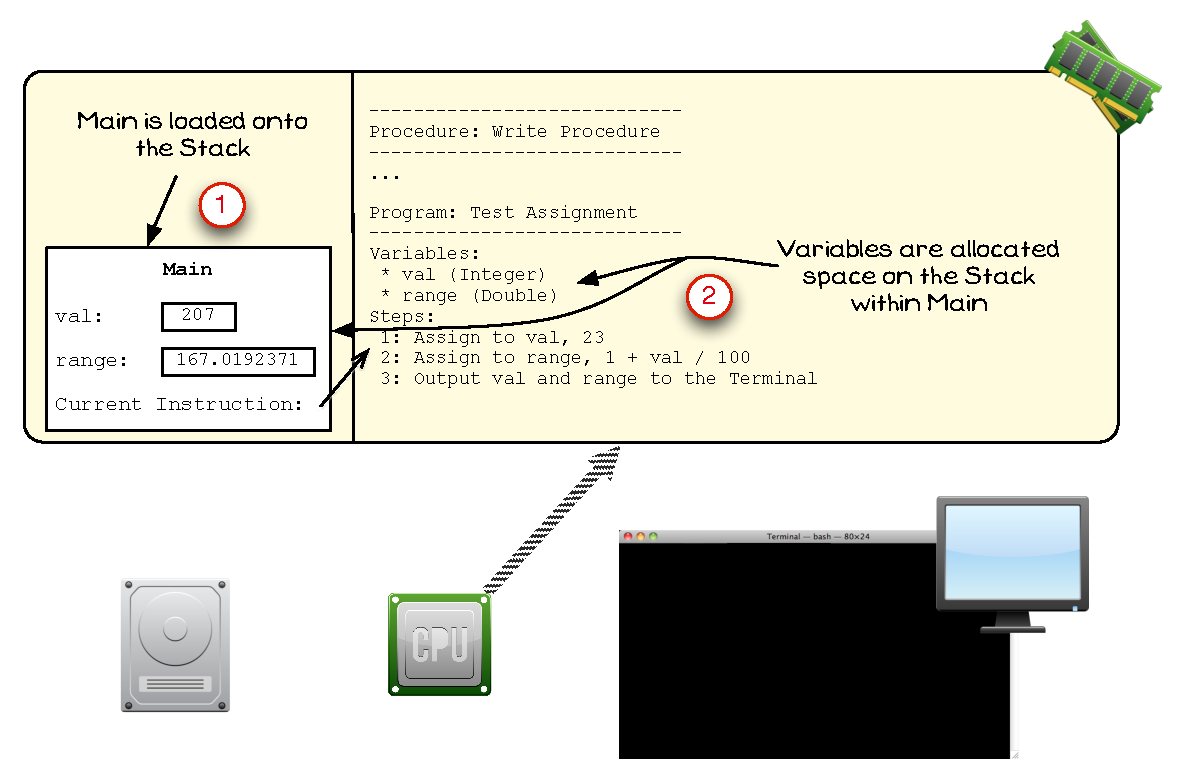
\includegraphics[width=\textwidth]{./topics/storing-using-data/images/vis-local-var-1} 
   \caption{Program's entry point is loaded onto the Stack}
   \label{fig:vis-data-local-1}
\end{figure}

\mynote{
\begin{itemize}
  \item The Program's instructions are loaded into memory when the program is executed.
  \item In Figure \ref{fig:vis-data-local-1} the indicated areas show the following:
  \begin{enumerate}
    \item When the Program starts, \texttt{Main} is loaded onto the Stack. This keeps track of all of the details related to the execution of \texttt{Main}.
    \item The Variables that are declared in \texttt{Main} are allocated space on the Stack.
  \end{enumerate}
  \item The two aspects of the Variable are shown in the illustration. The \textbf{variable} is the box drawn next to its name. The \textbf{value} is then written within the Variable.
  \item Notice that the variables each have a value to start with, even though the code has not yet assigned a value. The variable is allocated memory into which its value will be stored. \textbf{Memory is not automatically cleared} after its use, so the variables will get whatever value happened to be at that location previously.
  \item Each Variable is allocated enough space to stores its value. The \texttt{val} Variable needs 32 bits to store an \texttt{Integer} value, whereas the \texttt{range} Variable needs 64 bits to store its \texttt{Double} value.
\end{itemize}
}

% subsubsection test_assignment_s_program_launches_putting_main_on_the_stack_ (end)
\clearpage
\subsubsection{The assignment statement stores a value in the \texttt{val} Variable.} % (fold)
\label{ssub:the_assignment_statement_stores_a_value_in_the_val_variable_}

The first action of this program is to store the value 23 in the \texttt{val} Variable.

\begin{figure}[htbp]
   \centering
   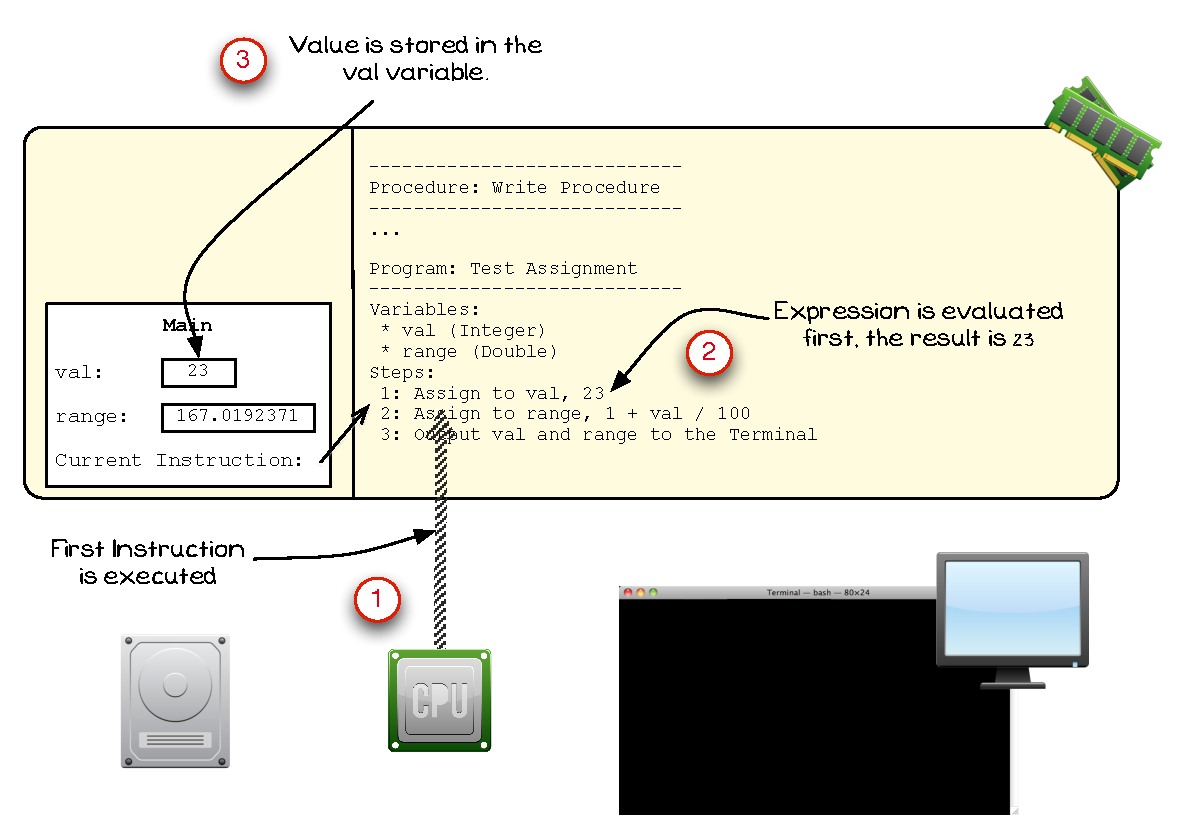
\includegraphics[width=\textwidth]{./topics/storing-using-data/images/vis-local-var-2} 
   \caption{The Assignment Statement assigns a value to the \texttt{val} Variable}
   \label{fig:vis-data-local-2}
\end{figure}

\mynote{
\begin{itemize}
  \item In Figure \ref{fig:vis-data-local-2} the indicated areas show the following:
  \begin{enumerate}
    \item The \nameref{sub:assignment_statement} is executed. This code has two sides. The right hand side executes first and needs to evaluate the Expression. Next the left hand side is used to determine where the resulting value needs to be stored.
    \item The value of the Expression is the Literal value 23.
    \item 23 is stored in the \texttt{val} Variable.
  \end{enumerate}
  \item Once this line of the Program has executed the \texttt{val} variable now has the value 23.
\end{itemize}
}

% subsubsection the_assignment_statement_stores_a_value_in_the_val_variable_ (end)

\clearpage
\subsubsection{The second assignment statements stores a value in the \texttt{range} Variable.} % (fold)
\label{ssub:the_second_assignment_statements_stores_a_value_in_the_range_variable_}

The next step in the program is to store the value \texttt{1 + val / 100} in the \texttt{range} Variable. This must read the value from the \texttt{val} Variable to determine the value to be stored.

\begin{figure}[htbp]
   \centering
   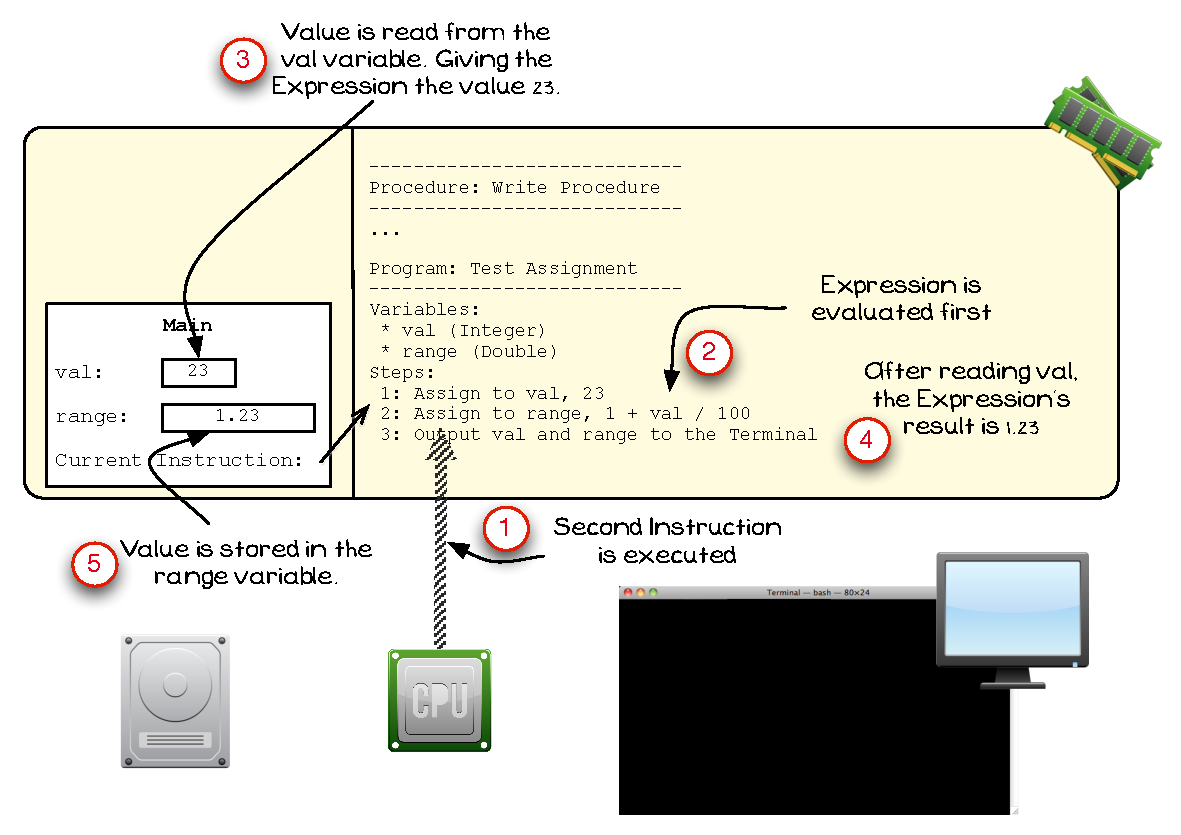
\includegraphics[width=\textwidth]{./topics/storing-using-data/images/vis-local-var-3} 
   \caption{The Assignment Statement assigns a value to the \texttt{val} Variable}
   \label{fig:vis-data-local-3}
\end{figure}

\mynote{
\begin{itemize}
  \item In Figure \ref{fig:vis-data-local-3} the indicated areas show the following:
  \begin{enumerate}
    \item The \nameref{sub:assignment_statement} is executed. As before, this needs to evaluate the Expression on the right hand side and store the result in the Variable on the left hand side.
    \item The first step to performing the assignment is to evaluate the expression. This requires the value from the \texttt{val} Variable.
    \item Within the Expression the value of \texttt{val} is read. At this point in the Program \texttt{val} has the value 23.
    \item The Expression is now \texttt{1 + 23 / 100}, giving the result \texttt{1.23}.
    \item The calculated value is then stored in the \texttt{range} Variable.
  \end{enumerate}
\end{itemize}
}

% subsubsection the_second_assignment_statements_stores_a_value_in_the_range_variable_ (end)

\clearpage
\subsubsection{The values of the Variables are output to the Terminal.} % (fold)
\label{ssub:the_values_of_the_variables_are_output_to_the_terminal_}

The third, and final, instruction in the Program's main function or procedure is to output the values of each of these variables to the Terminal. This uses the values from within the Variables to determine what is output.

\begin{figure}[htbp]
   \centering
   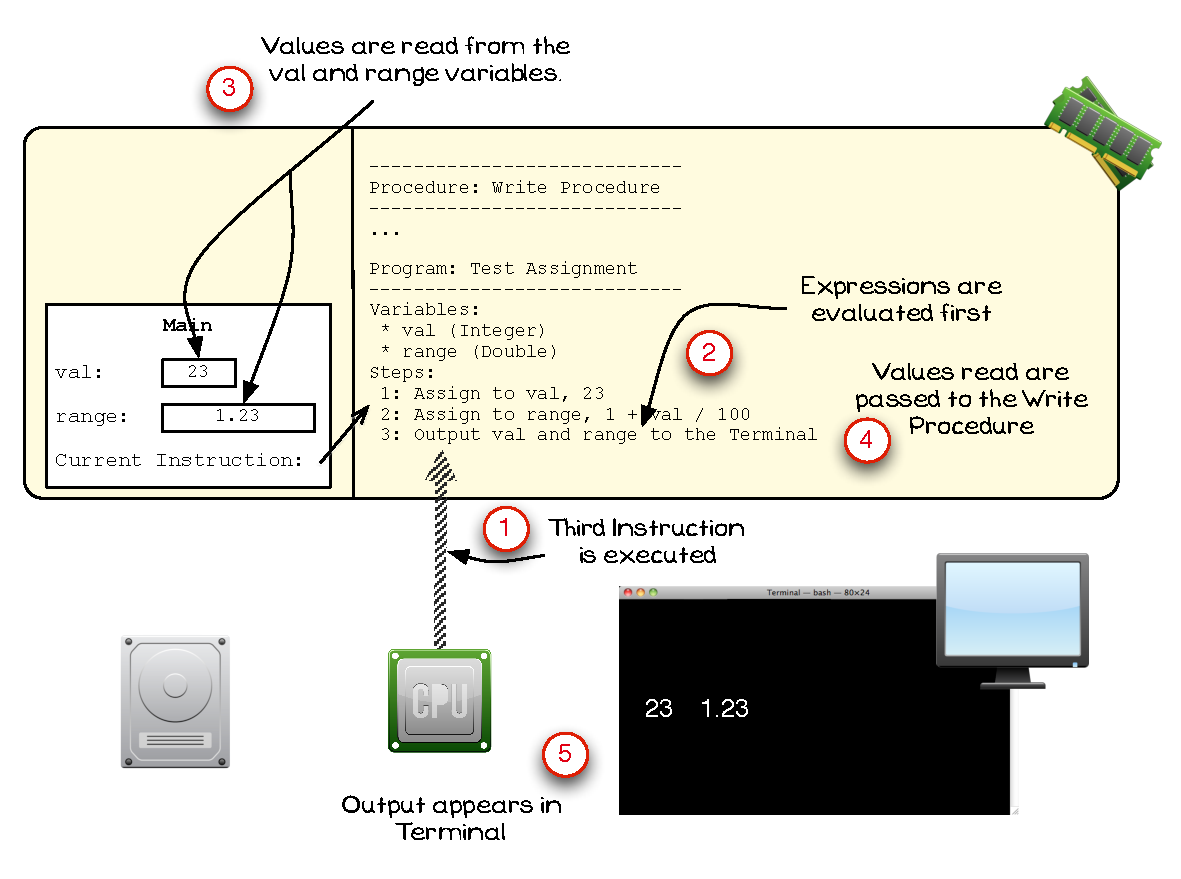
\includegraphics[width=\textwidth]{./topics/storing-using-data/images/vis-local-var-4} 
   \caption{The Assignment Statement assigns a value to the \texttt{val} Variable}
   \label{fig:vis-data-local-4}
\end{figure}

\mynote{
\begin{itemize}
  \item In Figure \ref{fig:vis-data-local-4} the indicated areas show the following:
  \begin{enumerate}
    \item The final instruction is a call to the output procedure of the language. This must be passed the data to output.
    \item The Write Procedure is passed a number of values to output.
    \item The values of the Variables will be read to get the argument values to pass.
    \item The values read from the Variables are then passed to the Write Procedure (\texttt{printf} in C, or \texttt{WriteLn} in Pascal).
    \item When the \texttt{Write Procedure} finishes its task the values will have been written to the Terminal.
  \end{enumerate}
\end{itemize}
}
% subsubsection the_values_of_the_variables_are_output_to_the_terminal_ (end)
% subsection local_variables (end)

\clearpage
\subsection{Parameters, Locals and Globals} % (fold)
\label{sub:visualise_parameters}

There are three locations at which you can declare variables. \emph{Global Variables} are declared within the program, \emph{Local Variables} are declared within Functions and Procedures, and \emph{Parameters} are used to pass values into Functions and Procedures.

\pseudocode{plst:test_proc_data}{Pseudocode used to examine how Global Variables, Local Variables, and Parameters work}{topics/storing-using-data/application/test-globals-and-locals.txt}

Listing \ref{plst:test_proc_data} is the code that we will use to demonstrate how these Variables work when code is executed by the Computer. This program does not have any meaningful purpose beyond interacting with Global Variables, Local Variables, and Parameters, so do not read too much into the actions being performed. What is important is to examine how the different variables work when the code is executed.

This Section will examine these Variables by looking at the following:
\begin{itemize}
  \item \nameref{ssub:memory_partitions_include_space_for_global_variables}
  \item \nameref{ssub:vars-program_is_loaded_into_memory}
  \item \nameref{ssub:initial_commands_occur}
  \item \nameref{ssub:passing_parameters_in_a_procedure_call}
  \item \nameref{ssub:test_params_commands_are_executed}
  \item \nameref{ssub:control_returns_to_main_when_test_params_ends}
\end{itemize}

\clearpage
\subsubsection{Memory Partitions include space for Global Variables} % (fold)
\label{ssub:memory_partitions_include_space_for_global_variables}

When the program is executed the Operating System allocates it space in memory. This space is partitioned into different areas, with each area storing an aspect of the program's data or instructions.

\begin{figure}[htbp]
   \centering
   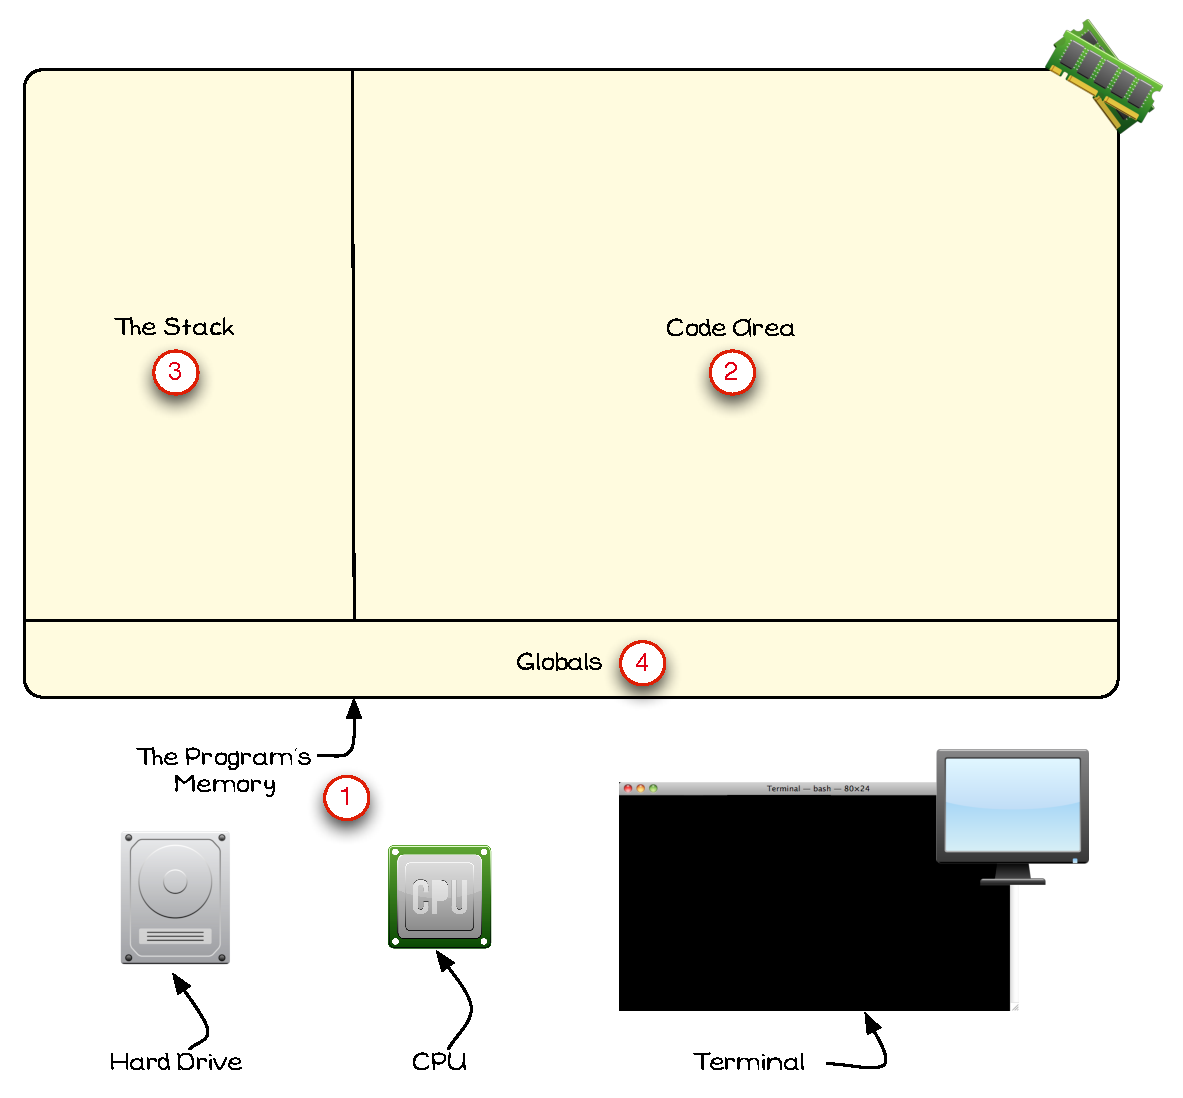
\includegraphics[width=0.9\textwidth]{./topics/storing-using-data/images/vis-globals-1} 
   \caption{Memory is partitioned into spaces for the Code, Stack, and Global Variables}
   \label{fig:vis-globals-1}
\end{figure}

\mynote{
\begin{itemize}
  \item In Figure \ref{fig:vis-globals-1} the indicated areas show the following:
  \begin{enumerate}
    \item The Program's memory is allocated by the Operation System, and divided into areas to store different kinds of values.
    \item The Program's instructions are loaded into the \textbf{Code Area}.
    \item The \textbf{Stack} is used to manage the execution of Functions and Procedures.
    \item \textbf{Global} Variables are stored in their own area of memory.
  \end{enumerate}
\end{itemize}
}

% subsubsection memory_partitions_include_space_for_global_variables (end)

\clearpage

\subsubsection{Program is loaded into memory} % (fold)
\label{ssub:vars-program_is_loaded_into_memory}

When the program is executed its global variables are allocated space, and then the main code is executed.

\begin{figure}[htbp]
   \centering
   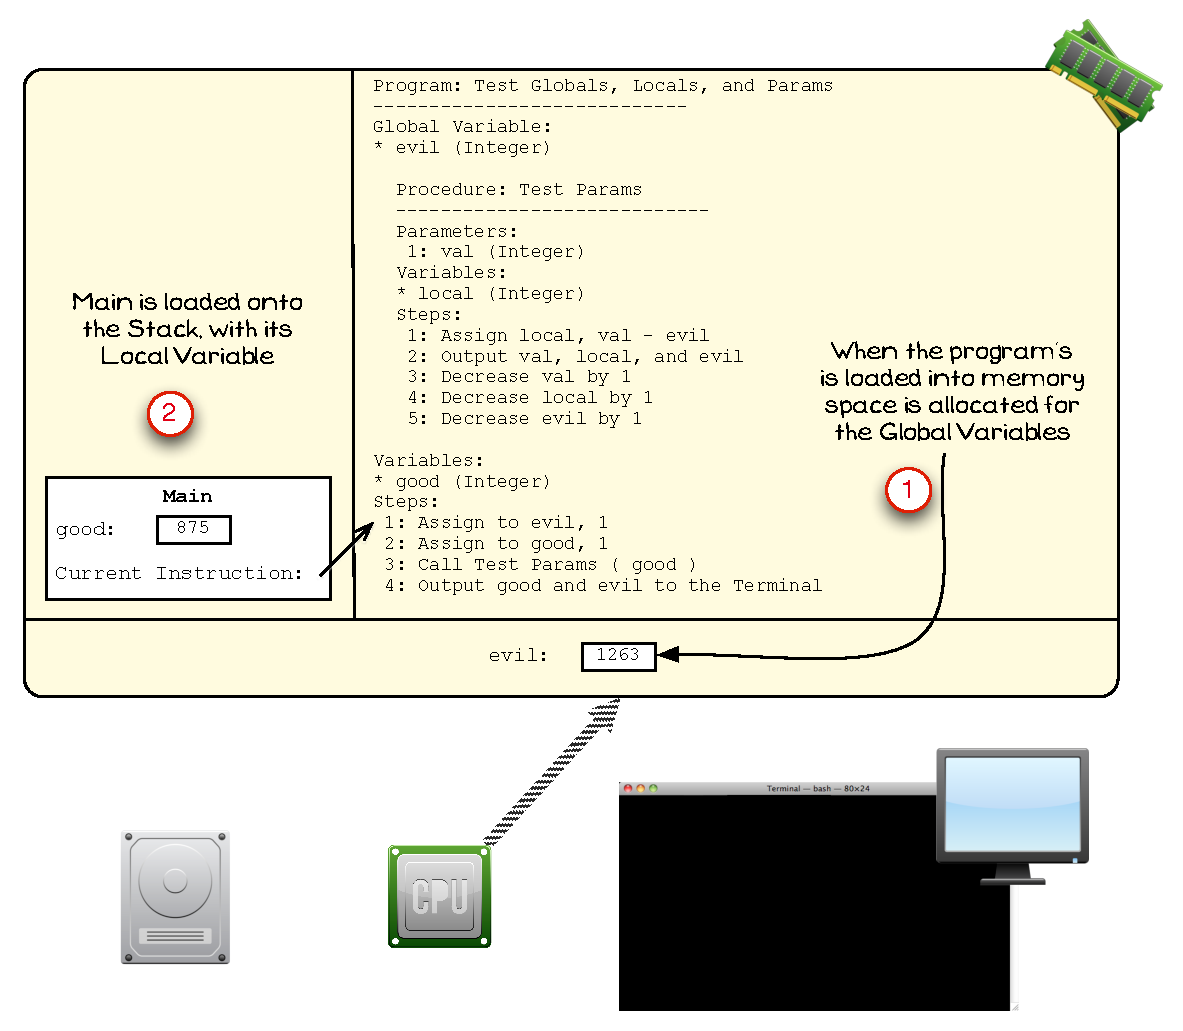
\includegraphics[width=\textwidth]{./topics/storing-using-data/images/vis-globals-2} 
   \caption{The Global Variables are allocated space, then the Entry Point is loaded onto the Stack}
   \label{fig:vis-globals-2}
\end{figure}

\mynote{
\begin{itemize}
  \item In Figure \ref{fig:vis-globals-2} the indicated areas show the following:
  \begin{enumerate}
    \item The global variables are allocated space when the program is loaded. Some Operating Systems ensure that this memory is cleared by zeroing each value, but others do not so you cannot rely upon the value these variables will have when they are loaded unless you initialise it yourself with an Assignment Statement.
    \item The main code is then loaded onto the Stack, with space for its local variable.
  \end{enumerate}
\end{itemize}
}

% subsection program_is_loaded_into_memory (end)
\clearpage

\subsubsection{Initial Commands Occur} % (fold)
\label{ssub:initial_commands_occur}

The program executes each of the statements, one at a time. Figure \ref{fig:vis-globals-3} shows the values in memory by the time the Computer has completed the execution of the first two commands.

\begin{figure}[htbp]
   \centering
   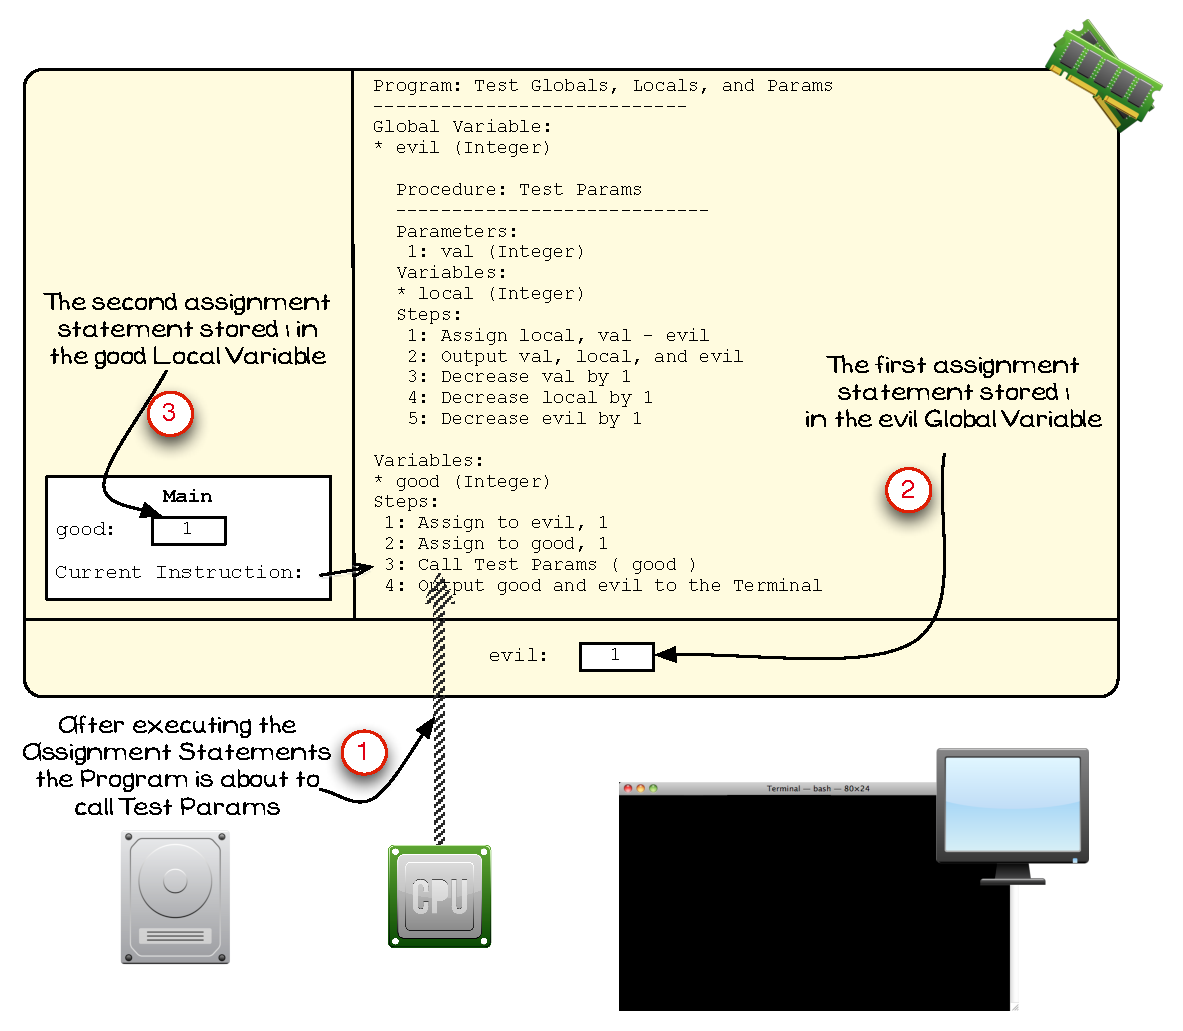
\includegraphics[width=\textwidth]{./topics/storing-using-data/images/vis-globals-3} 
   \caption{The instructions store values in the different variables}
   \label{fig:vis-globals-3}
\end{figure}

\mynote{
\begin{itemize}
  \item In Figure \ref{fig:vis-globals-3} the indicated areas show the following:
  \begin{enumerate}
    \item This picture is showing the computer at the point just before it executes the call to \texttt{Test Params}.
    \item The first assignment statement assigned the value \texttt{1} to the \texttt{evil} Global Variable.
    \item The second assignment statement assigned the value \texttt{1} to the \texttt{good} Local Variable.
  \end{enumerate}
\end{itemize}
}

% subsubsection initial_commands_occur (end)

\clearpage

\subsubsection{Passing Parameters in a Procedure Call} % (fold)
\label{ssub:passing_parameters_in_a_procedure_call}

At this point the Computer is executing the call to \texttt{Test Params}. This involves passing a value to the \texttt{val} parameter.

\begin{figure}[htbp]
   \centering
   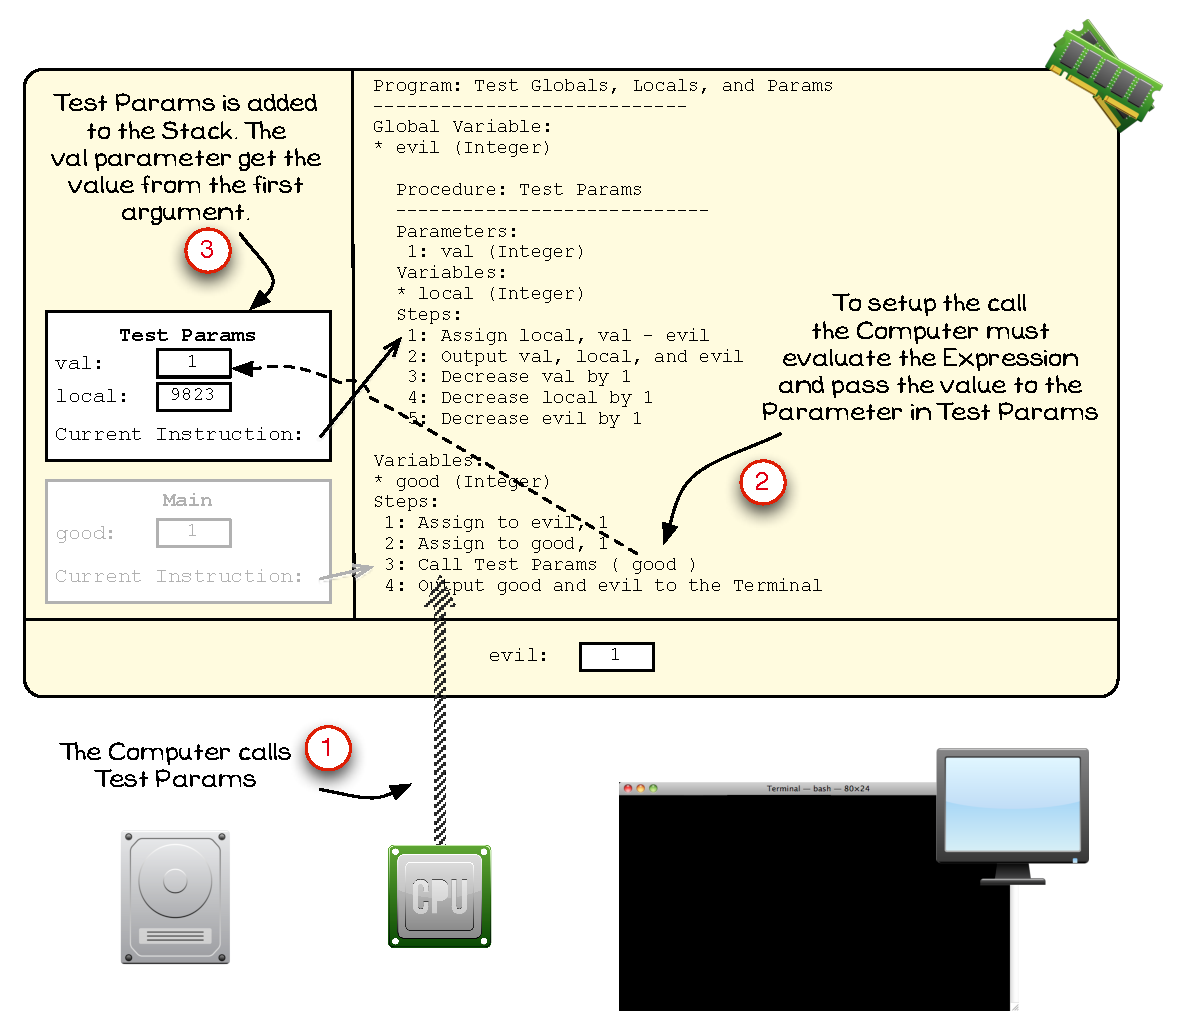
\includegraphics[width=\textwidth]{./topics/storing-using-data/images/vis-globals-4} 
   \caption{The \emph{value} of the Argument is passed to the Parameter when the Procedure is called}
   \label{fig:vis-globals-4}
\end{figure}

\mynote{
\begin{itemize}
  \item In Figure \ref{fig:vis-globals-4} the indicated areas show the following:
  \begin{enumerate}
    \item The Computer calls the \texttt{Test Params} procedure. This must be passed a single value that will be copied into the \texttt{val} Parameter.
    \item The first part of the call requires the Computer to evaluate the Expression being passed to the Procedure. In this case that involves reading the \texttt{good} Local Variable and passing its \emph{value} to the Parameter.
    \item Once the values for the Parameters are determined, the next step is to allocate space for \texttt{Test Params} on the Stack. Within \texttt{Test Params} there will be space allocated for the \texttt{val} parameter, as well as space allocated for the \texttt{local} Local Variable. The value of the \emph{argument} is copied into the \emph{parameter}, and the called Function or Procedure's code can now execute. In this case the value \texttt{1} is stored in \texttt{val}.
  \end{enumerate}
\end{itemize}
}


% subsubsection passing_parameters_in_a_procedure_call (end)
\clearpage

\subsubsection{Test Params Commands are Executed} % (fold)
\label{ssub:test_params_commands_are_executed}

The commands in \texttt{Test Params} are executed one at a time. These instructions will interact with the Variables that are visible to the \texttt{Test Params} Procedure, which include its Local Variables as well as the Global Variables.

\begin{figure}[htbp]
   \centering
   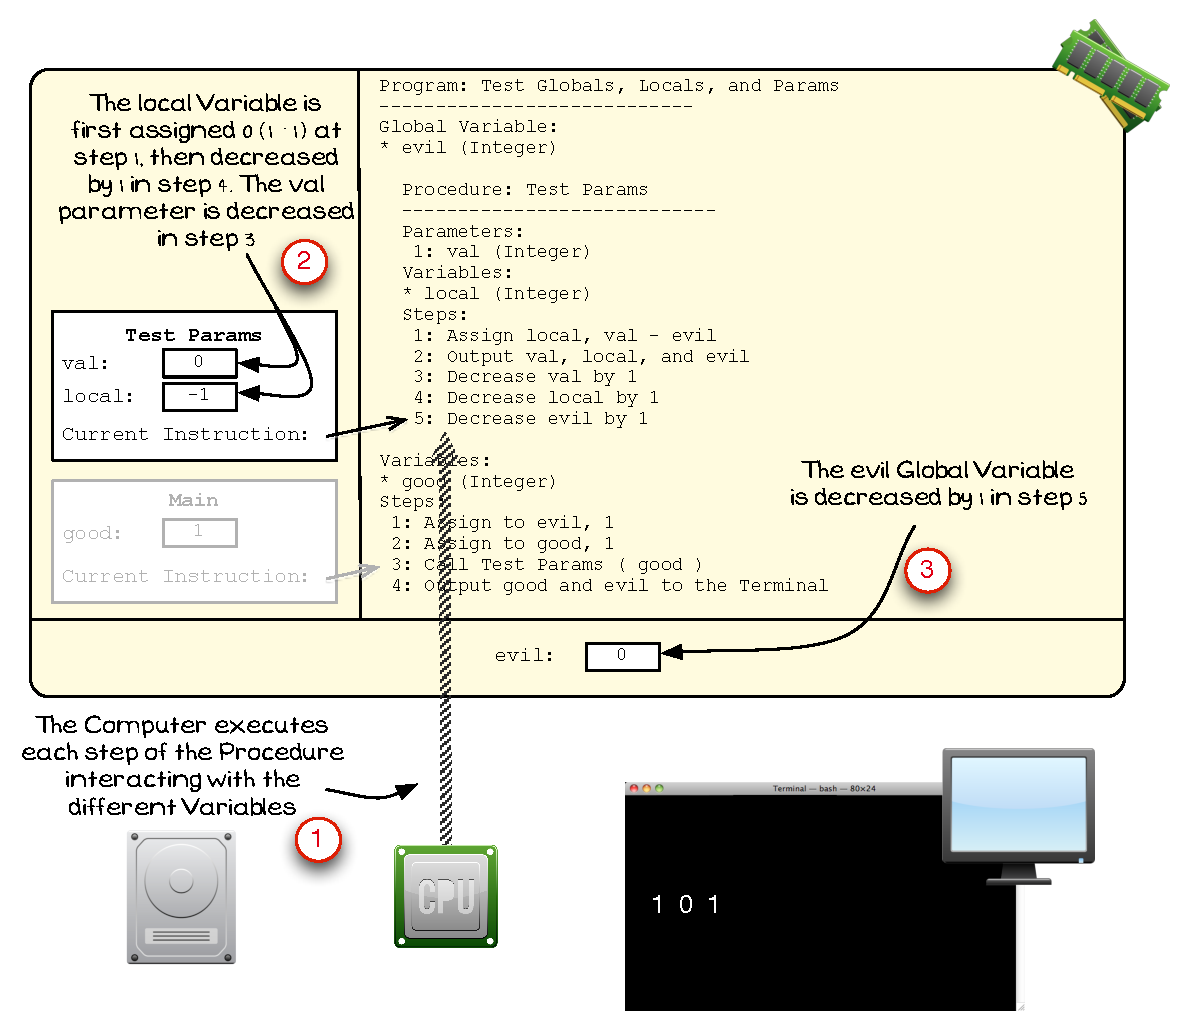
\includegraphics[width=\textwidth]{./topics/storing-using-data/images/vis-globals-5} 
   \caption{Steps in \texttt{Test Params} execute, altering values in the Variables}
   \label{fig:vis-globals-5}
\end{figure}

\mynote{
\begin{itemize}
  \item In Figure \ref{fig:vis-globals-5} the indicated areas show the following:
  \begin{enumerate}
    \item Each instruction is executed one at a time. This picture shows the instructions at the end of the last instruction in \texttt{Test Params} before it ends.
    \item The steps of the Procedure are able to read and write values to the Function or Procedure's Parameters and Local Variables, as shown here.
    \item The Procedure is also able to read and write values to the Global Variables.
  \end{enumerate}
  \item Notice that \texttt{Test Params} cannot see the \texttt{good} Variable. It exists within the \texttt{Main} code and cannot be accessed from other Functions or Procedures.
  \item You can decrease the value of a Variable using an Assignment Statement. For example `\texttt{Assign to val, the value val - 1}'. This will read the current value from the \texttt{val} Variable, subtract one from that, and then store the result back in the \texttt{val} variable.
\end{itemize}
}
% subsubsection test_params_commands_are_executed (end)

\clearpage

\subsubsection{Control returns to Main when Test Params ends} % (fold)
\label{ssub:control_returns_to_main_when_test_params_ends}

When \texttt{Test Params} ends control returns to the Program's main code. The space allocated to \texttt{Test Params} is now released, including the space allocated to the \texttt{val} Parameter and the \texttt{local} Variable.

\begin{figure}[htbp]
   \centering
   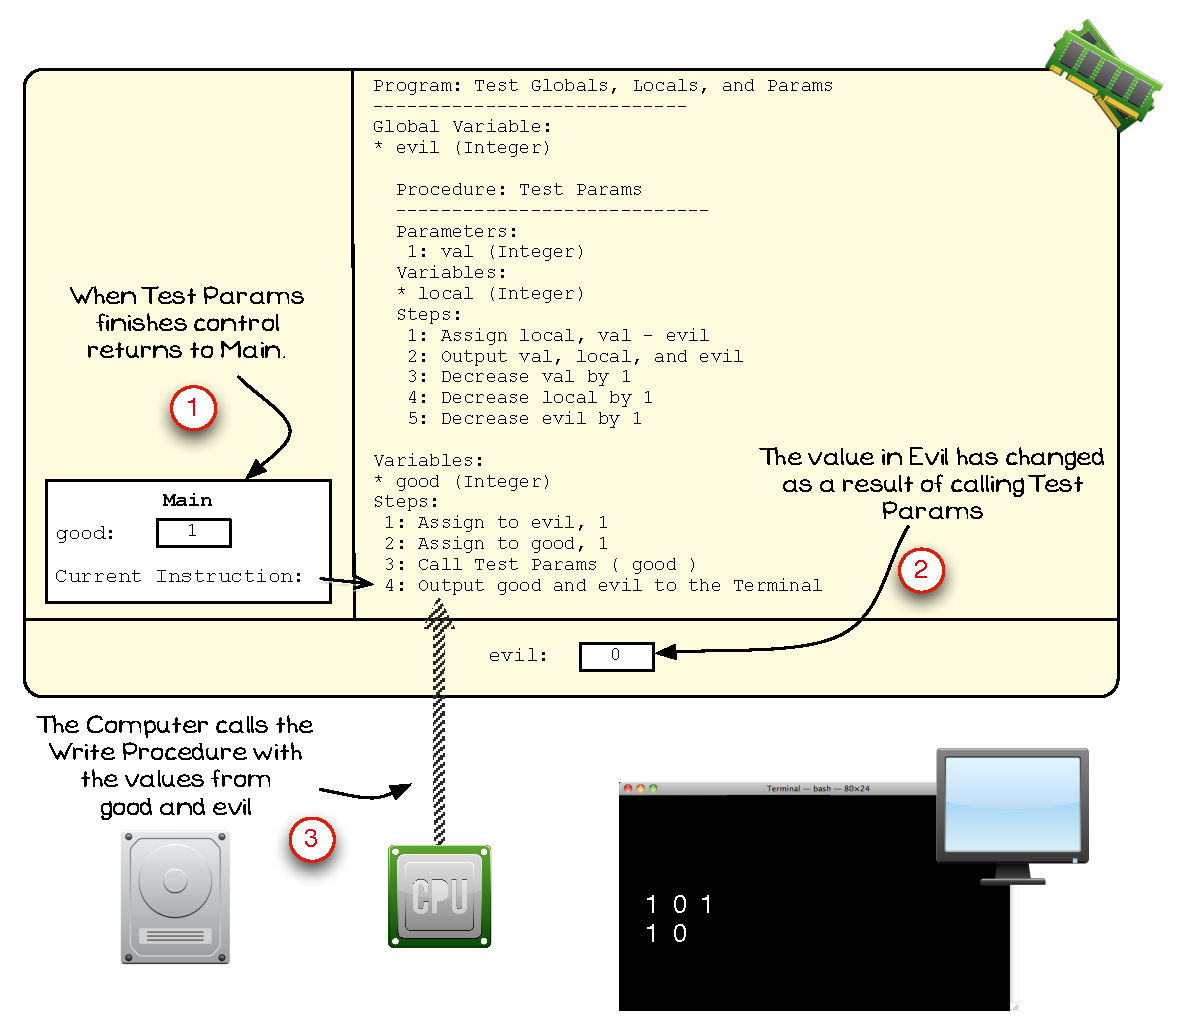
\includegraphics[width=\textwidth]{./topics/storing-using-data/images/vis-globals-6} 
   \caption{Control returns to Main when \texttt{Test Params} ends}
   \label{fig:vis-globals-6}
\end{figure}

\mynote{
\begin{itemize}
  \item In Figure \ref{fig:vis-globals-6} the indicated areas show the following:
  \begin{enumerate}
    \item Control returns to \texttt{Main} when \texttt{Test Params} ends.
    \item Notice that the value of the \texttt{evil} Global Variable has changed as a side effect of running \texttt{Test Params}. This is easy to follow in a small program, but can cause difficulties when you start building larger programs. As a result, Global Variables should be avoided.
    \item The last instruction in the main code outputs the values of \texttt{good} and \texttt{evil} to the Terminal.
  \end{enumerate}
  \item The value within \texttt{good} has been passed to the \texttt{val} Parameter in \texttt{Test Params}. This copies the \emph{value}, not the \texttt{Variable}, as it is using the standard \emph{Pass by Value} mechanism. This means the code in \texttt{Test Params} has no way of affecting the value in the \texttt{good} Variable.
\end{itemize}
}

% subsection control_returns_to_main_when_test_params_ends (end)
\clearpage

% subsection parameters (end)

\subsection{Function Return Values} % (fold)
\label{sub:visualise_function_return_values}

The next kind of data is the result returned by a call to a Function. A Function is just like a Procedure, except that it calculates a value and is therefore called from within an Expression. To examine how this works within the Computer we will see how the code in Listing \ref{plst:function-test} executes. This code declares a \texttt{Square} function that calculates the square of a number (\texttt{val} passed in as a Parameter).   

\pseudocode{plst:function-test}{Function example, to illustrate how data is returned from a Function}{topics/storing-using-data/application/test-function.txt}

This Section will examine how Functions return values by looking at the following:
\begin{itemize}
  \item \nameref{ssub:test_functions_is_loaded_into_memory}
  \item \nameref{ssub:square_function_is_called}
  \item \nameref{ssub:square_s_result_is_calculated}
  \item \nameref{ssub:returned_value_is_used}
\end{itemize}

\clearpage
\subsubsection{Test Functions is loaded into memory} % (fold)
\label{ssub:test_functions_is_loaded_into_memory}

When the program is executes the Operating System loads its code into memory, and starts the main code running on the Stack.

\begin{figure}[htbp]
   \centering
   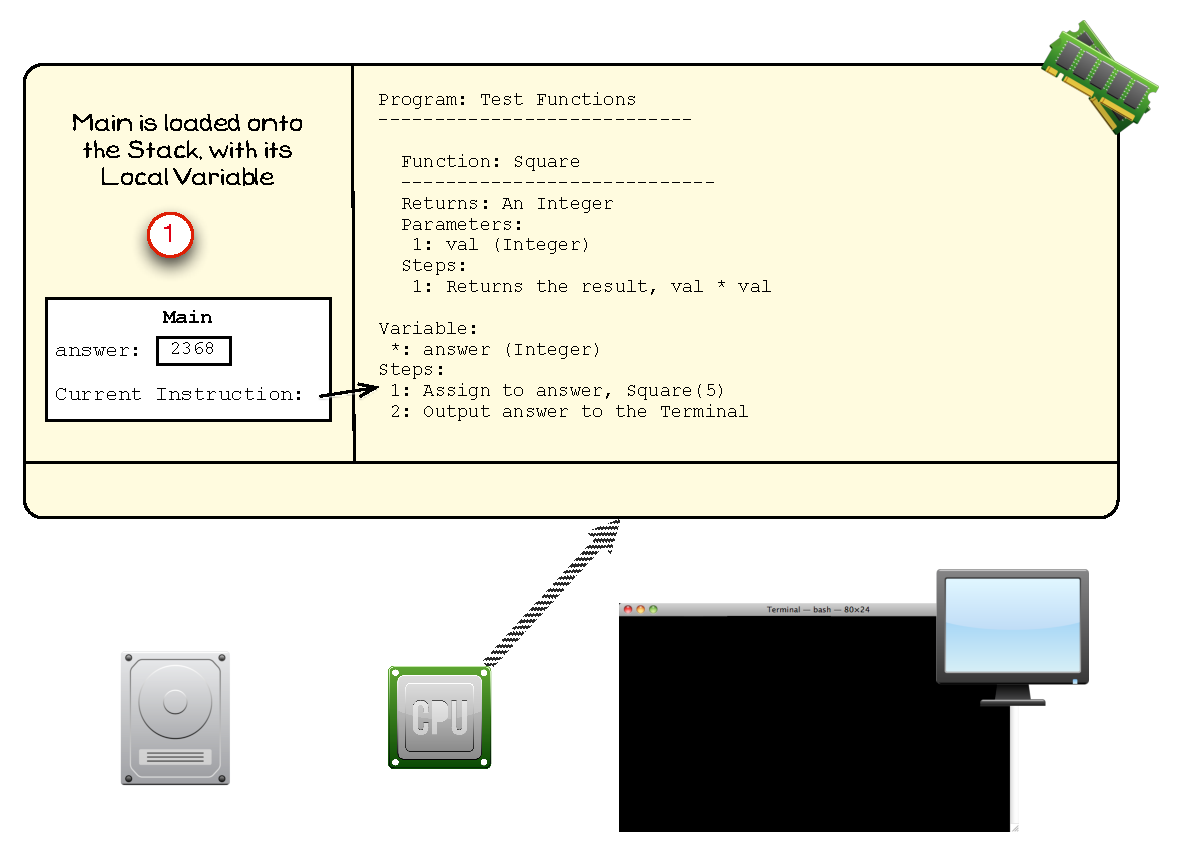
\includegraphics[width=\textwidth]{./topics/storing-using-data/images/vis-func-1} 
   \caption{Code is loaded into Memory and Main is loaded onto the Stack}
   \label{fig:vis-func-1}
\end{figure}

\mynote{
\begin{itemize}
  \item In Figure \ref{fig:vis-func-1} the indicated areas show the following:
  \begin{enumerate}
    \item Main is loaded onto the Stack, with space for its \texttt{answer} local variable.
  \end{enumerate}
  \item Notice the Global Variables section is empty as this program does not use Global Variables.
\end{itemize}
}

% subsubsection test_functions_is_loaded_into_memory (end)

\clearpage

\subsubsection{Square Function is Called} % (fold)
\label{ssub:square_function_is_called}

The \texttt{Square} function is called in the same way that a Procedure would be called. It is given space on the Stack, and its instructions are run.

\begin{figure}[htbp]
   \centering
   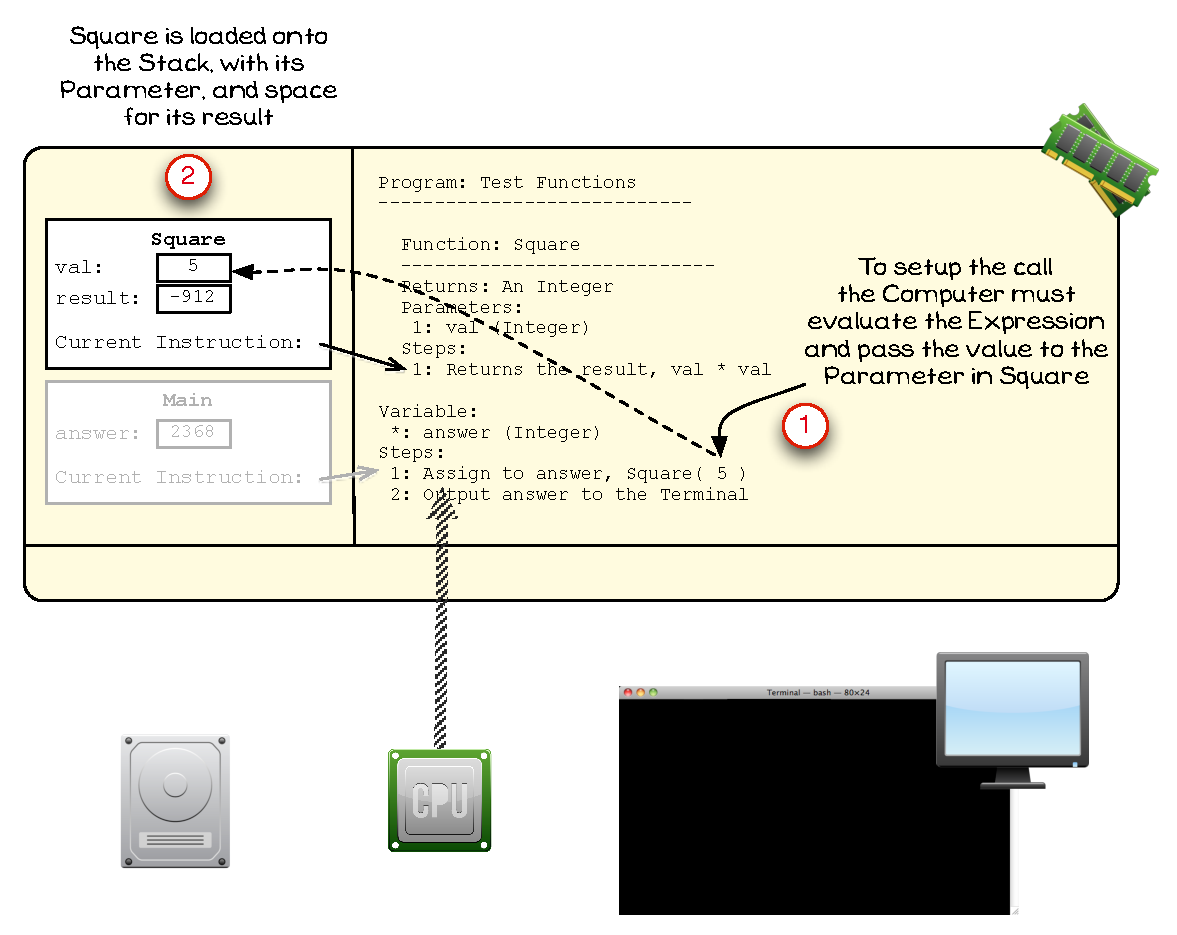
\includegraphics[width=\textwidth]{./topics/storing-using-data/images/vis-func-2} 
   \caption{\texttt{Square} is called, with the value 5 passed to its \texttt{val} Parameter}
   \label{fig:vis-func-2}
\end{figure}

\mynote{
\begin{itemize}
  \item In Figure \ref{fig:vis-func-2} the indicated areas show the following:
  \begin{enumerate}
    \item When the main code calls \texttt{Square} it passed in the value \texttt{5}, calculated simply by reading the Literal value.
    \item \texttt{Square} is added to the top of the Stack, and its \texttt{val} parameter is assigned the value passed in from the Function Call. In addition to any Parameter and Local Variables the Function also has space for its \texttt{result}. This will be the value returned to the caller when the Function ends.
  \end{enumerate}
  \item The value of the result will initially be whatever happens to be at that location in memory the last time it was used. You must make sure you assign a value to this within the Function.
\end{itemize}
}

\csection{In C the \nameref{sub:return_statement} assigns the value returned by the Function. There is no special \texttt{result} Variable that you can interact with. Conceptually, however, the value must be stored in order to be returned by the Function. In C the compiler takes care of these details for you.}



% subsubsection square_function_is_called (end)

\clearpage

\subsubsection{Square's result is calculated} % (fold)
\label{ssub:square_s_result_is_calculated}

Within the \texttt{Square} function its result is calculated and returned.

\begin{figure}[htbp]
   \centering
   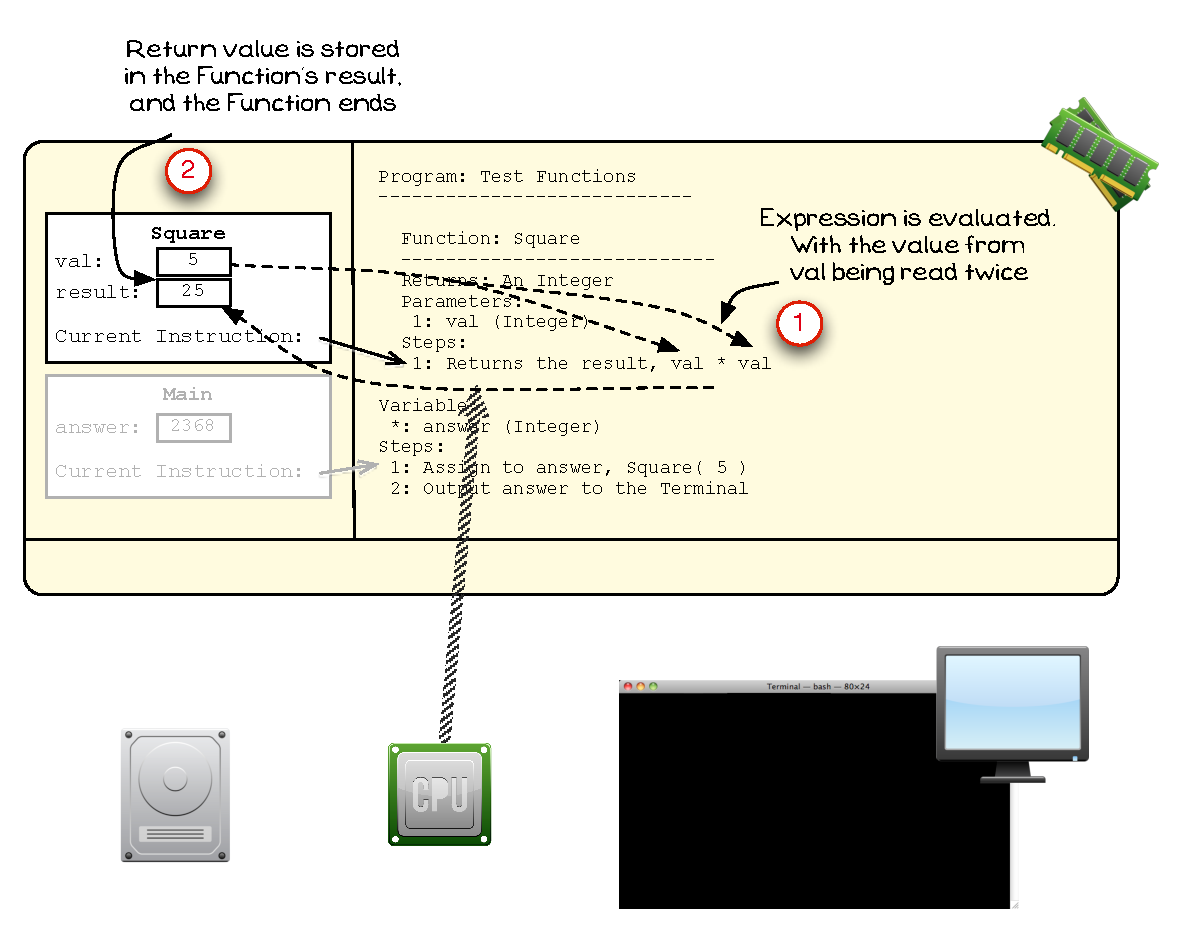
\includegraphics[width=\textwidth]{./topics/storing-using-data/images/vis-func-3} 
   \caption{\texttt{Square} prepares the value that will be returned to the caller}
   \label{fig:vis-func-3}
\end{figure}

\mynote{
\begin{itemize}
  \item In Figure \ref{fig:vis-func-3} the indicated areas show the following:
  \begin{enumerate}
    \item The expression `\texttt{val * val}' is evaluated. This reads the value of the \texttt{val} variable twice and multiplies the two values read. In this case this will calculate `\texttt{5 * 5}', giving \texttt{25}.
    \item The result of the expression is returned, setting the Function's result.
  \end{enumerate}
\end{itemize}
}

\csection{In C this is accomplished with the \nameref{sub:return_statement}. It assigns the result for the function and ends the Function at the same time.}

\passection{In Pascal you directly store the value in the special \texttt{result} Variable. This will not end the Function directly, but does store the value to be returned by the Function.}


% subsubsection square_s_result_is_calculated (end)
\clearpage

\subsubsection{Returned value is used} % (fold)
\label{ssub:returned_value_is_used}

When the Function ends, control is returned to the main code. This called the Function in order to evaluate an Expression. That expression will now continue to be evaluated using the value returned by the Function.

\begin{figure}[htbp]
   \centering
   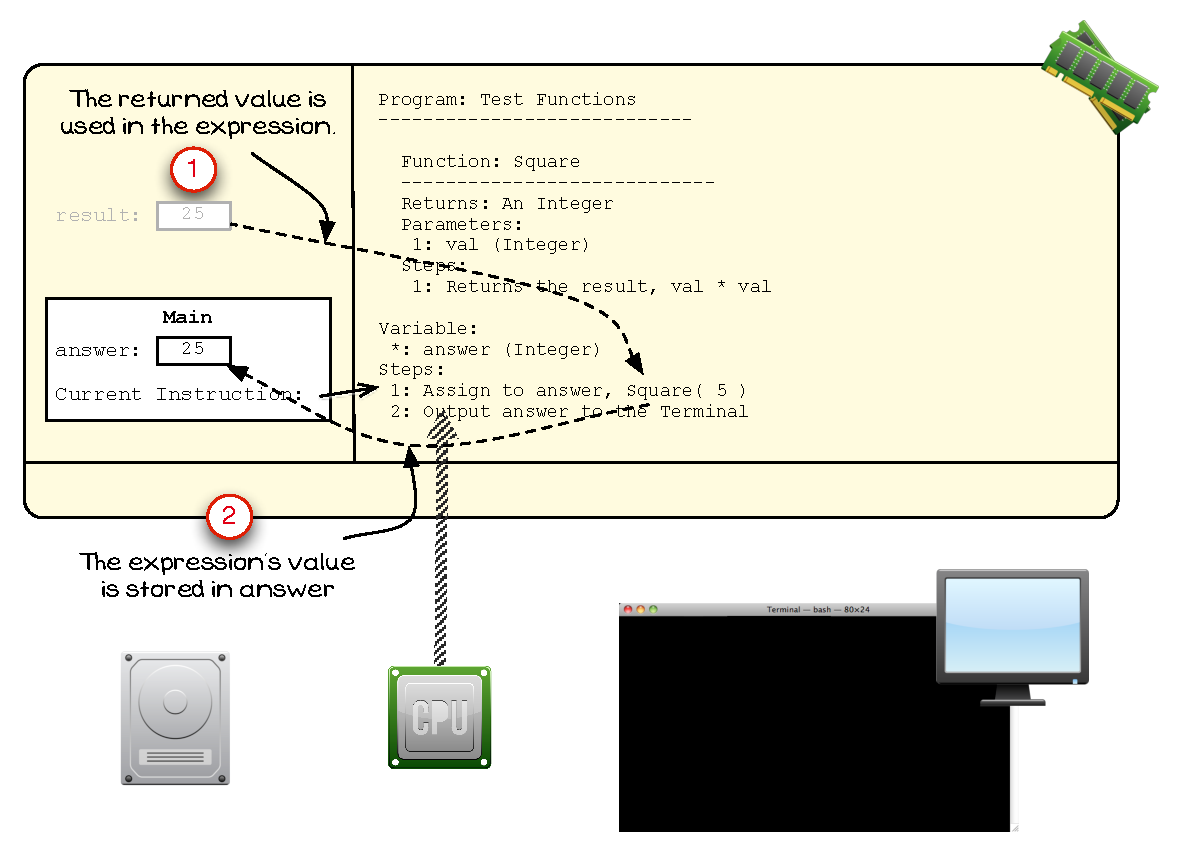
\includegraphics[width=\textwidth]{./topics/storing-using-data/images/vis-func-4} 
   \caption{The result of calling \texttt{Square} is used within the Expression, and the value is stored in \texttt{answer}}
   \label{fig:vis-func-4}
\end{figure}

\mynote{
\begin{itemize}
  \item In Figure \ref{fig:vis-func-4} the indicated areas show the following:
  \begin{enumerate}
    \item The result of the Function is made available to the caller. This will be read as part of the Function Call, and is then used within the Expression.
    \item In this case the Expression does not alter the value returned by the Function, and the result is stored in the \texttt{answer} variable.
  \end{enumerate}
  \item The expression that contains the Function Call can operate on the result returned from the function in the same way that it uses any other value. For example, the following expression is valid: \texttt{3 + Square(-7) * 5 + Square(Square(2))}.
  \item The key is to think of each Function Call as a value. So nested Function Calls like \texttt{Square(Square(2))} can be broken down into their individual values. In this example \texttt{Square(2)} is evaluated first, and returns the value \texttt{4}. This is then passed to the outer Function Call giving \texttt{Square(4)} and a final result of \texttt{16}.
\end{itemize}
}

% subsubsection returned_value_is_used (end)
% subsection function_return_values (end)

\clearpage
\subsection{Pass by Reference} % (fold)
\label{sub:visualise_pass_by_reference}

Working with data involves working with Variables of one form or another. When thinking about Variables it is important to realise the two aspects of each Variable: the \emph{Variable} and its \emph{value}. The \emph{Variable} is a location in memory, it is a place at which you can store a value. The \emph{value} within the Variable is a separate concern. This value can be read from the Variable in Expressions.

\pseudocode{plst:pass-by-ref-test}{Example used to illustrate how Pass by Reference works with the standard input Functions and Procedures.}{topics/storing-using-data/application/test-input.txt}

This Section will examine how Pass by Reference works by looking at the following:
\begin{itemize}
  \item \nameref{ssub:main_starts_and_a_prompt_is_written_for_the_user}
  \item \nameref{ssub:the_input_procedure_is_called_to_read_a_value_into_age}
  \item \nameref{ssub:the_input_procedure_stores_the_value_read_from_the_user_into_}
  \item \nameref{ssub:control_returns_to_main_and_}
\end{itemize}

\csection{In C the \texttt{Read Input Procedure} is the \texttt{scanf()} Function. This requires that you pass in a format string that indicates what will be read as well as passing in the Variables into which these values will be stored. You can read about this in \nameref{sub:c_terminal_input}. Step 2 from Listing \ref{plst:pass-by-ref-test} can be implemented in C using \csnipet{scanf("\%d", \&age);}.}

\clearpage
\subsubsection{Main starts and a prompt is written for the user} % (fold)
\label{ssub:main_starts_and_a_prompt_is_written_for_the_user}

The Program starts as normal with the Operating System allocating space for the Stack, Code, and Global Variables. Main is then loaded onto the Stack and its instructions are executed.

\begin{figure}[htbp]
   \centering
   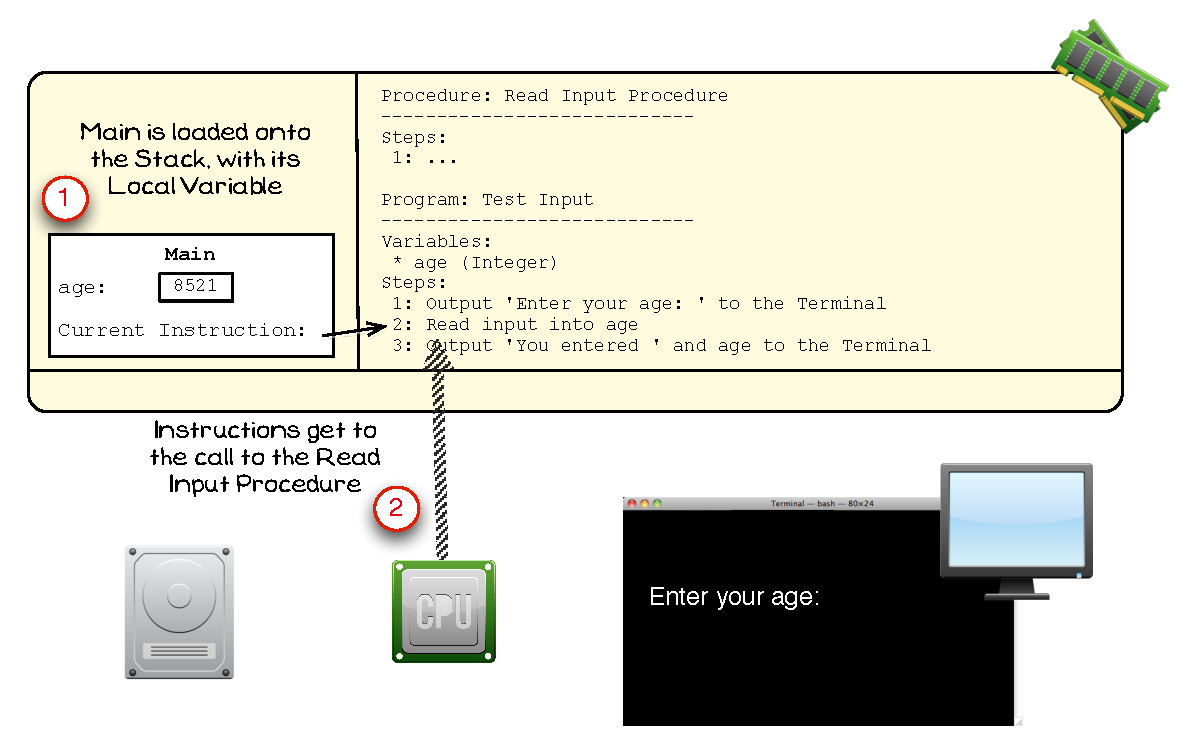
\includegraphics[width=\textwidth]{./topics/storing-using-data/images/vis-ref-1} 
   \caption{Code is loaded into Memory, Main is started, and the first instruction outputs a prompt}
   \label{fig:vis-ref-1}
\end{figure}

\mynote{
\begin{itemize}
  \item In Figure \ref{fig:vis-ref-1} the indicated areas show the following:
  \begin{enumerate}
    \item Main is loaded onto the stack, with space for the \texttt{age} Variable.
    \item The first instruction outputs `Enter your age: ' to the Terminal.
  \end{enumerate}
  \item When writing a prompt it is a good idea to keep the output on a single line. Just write the prompt without writing a new line.
\end{itemize}
}

% subsubsection main_starts_and_a_prompt_is_written_for_the_user (end)

\clearpage
\subsubsection{The Input Procedure is called to read a value into \texttt{age}} % (fold)
\label{ssub:the_input_procedure_is_called_to_read_a_value_into_age}

The next instruction in the main code is to call the Language's input procedure to read a value from the user and to store that value in the \texttt{age} variable. In order to achieve this you must pass the \texttt{age} variable itself to this procedure. That will enable the input code to store the value it reads into the variable that you give it.

\begin{figure}[htbp]
   \centering
   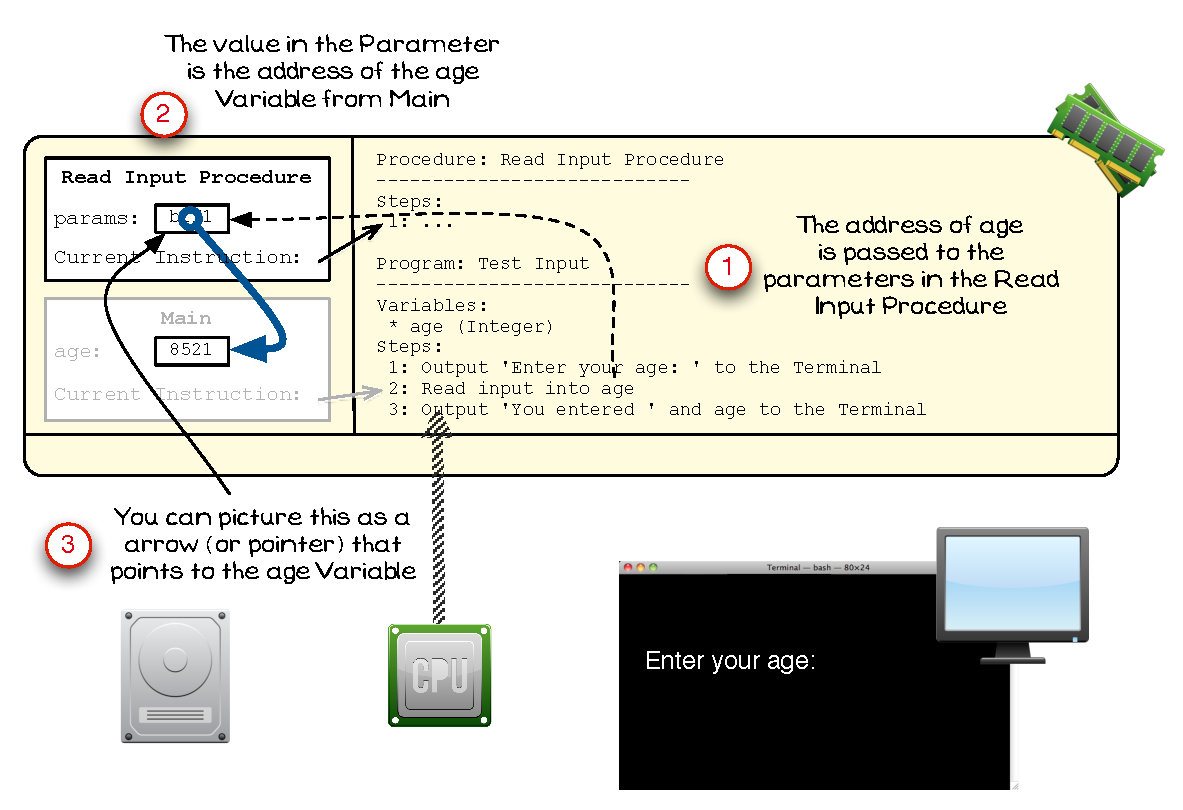
\includegraphics[width=\textwidth]{./topics/storing-using-data/images/vis-ref-2} 
   \caption{The input procedure starts, and the age Variable is passed to the Parameters}
   \label{fig:vis-ref-2}
\end{figure}

\mynote{
\begin{itemize}
  \item In Figure \ref{fig:vis-ref-2} the indicated areas show the following:
  \begin{enumerate}
    \item A variable is a location in memory, so it is not possible to actually move this location into the Parameter. What happens instead is that you pass the \textbf{address} of the Variable to the Parameter. This is why it is commonly called \emph{Pass by Reference}, you are passing a reference to the Variable, in effect telling it where the Variable is that you want the data stored in.
    \item The value passed to the Parameter is then the \emph{address} of the Variable where the data should be stored. This Parameter is now storing the location of the \texttt{age} Variable.
    \item An good way to picture this is as an arrow, or a pointer, that points from value within the Parameter to the \texttt{age} Variable. This helps visualise the fact that this Parameter is storing the location of the \texttt{age} Variable.
  \end{enumerate}
\end{itemize}
}

\csection{In C you must manually get the address of the variable using the ampersand (\&) operator. So the call \csnipet{scanf("\%d", \&age);} in Main is passing the \emph{address} of \texttt{age}. You can read \texttt{\&age} as `\emph{The address of age}'.}

% subsubsection the_input_procedure_is_called_to_read_a_value_into_age (end)

\clearpage
\subsubsection{The Input Procedure stores the value read from the user into \texttt{age}} % (fold)
\label{ssub:the_input_procedure_stores_the_value_read_from_the_user_into_}

The language's input procedures are responsible for reading values from the user and storing these into Variables for you. The instructions in this code will do the work to convert the data from the text the user enters into the types required by the Variables the values are being read into.

\begin{figure}[htbp]
   \centering
   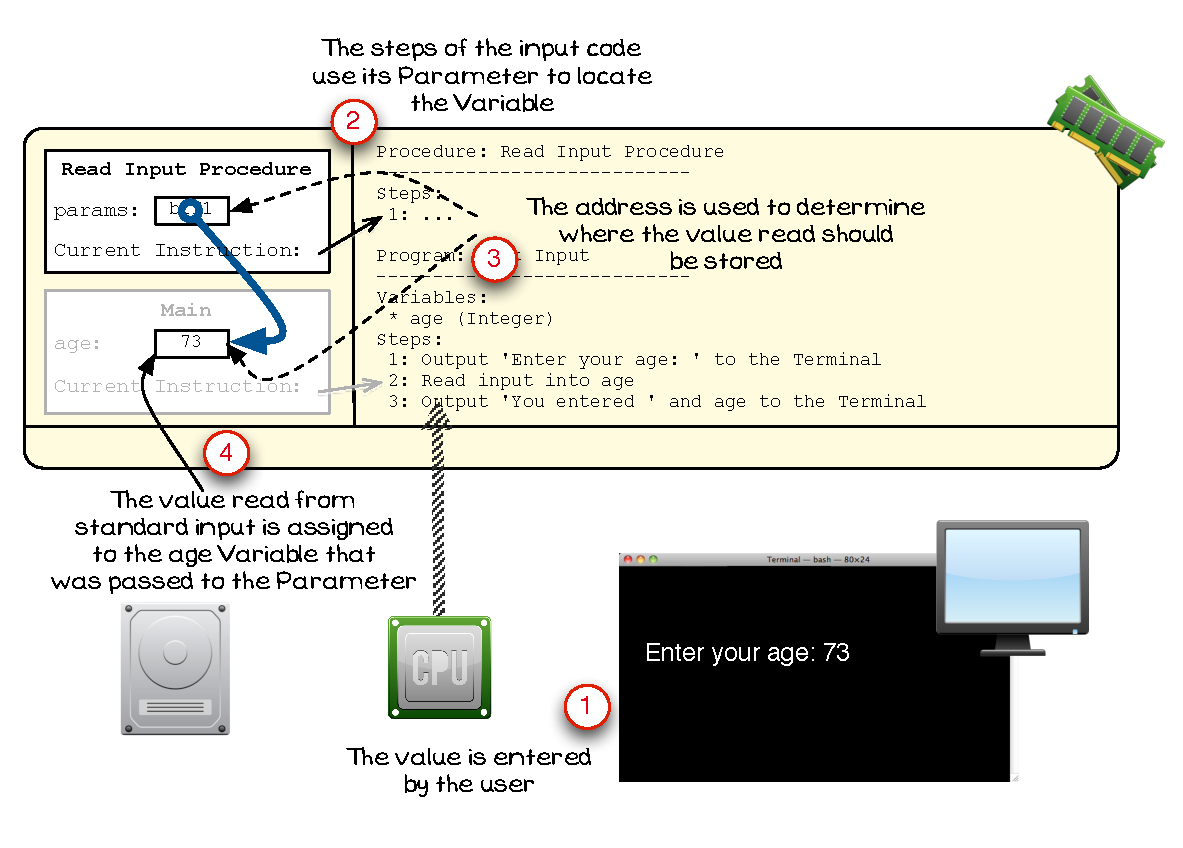
\includegraphics[width=\textwidth]{./topics/storing-using-data/images/vis-ref-3} 
   \caption{Within the input code the address is used to find where to store the value read from the user}
   \label{fig:vis-ref-3}
\end{figure}

\mynote{
\begin{itemize}
  \item In Figure \ref{fig:vis-ref-3} the indicated areas show the following:
  \begin{enumerate}
    \item The input code waits for the user to enter a value at the Terminal. Once the value is entered it is scanned and stored in the Variables passed to the Input Procedure.
    \item The input code needs to work out where the values read are to be stored. It does this by looking up the address stored in its Parameter.
    \item The address is used to locate the Variable into which the value will be stored.
    \item In this case the Parameter has the address of the \texttt{age} variable, and therefore the value read from the user is stored into Main's \texttt{age} Variable.
  \end{enumerate}
  \item The language's Input Procedures can be used to read in more than one value at a time. In these cases the inputs code will read values for each Variable one at a time.
\end{itemize}
}

\csection{In C you are responsible for determining how the data read is interpreted. This is the purpose of the \emph{format string} passed as the first parameter to \texttt{scanf}. In \csnipet{scanf("\%d", \&age);} the \texttt{"\%d"} indicates that the first Variable needs to be assigned a decimal integer value.}

% subsubsection the_input_procedure_stores_the_value_read_from_the_user_into_ (end)

\clearpage
\subsubsection{Control returns to Main and \texttt{age} has been updated with the value from the user} % (fold)
\label{ssub:control_returns_to_main_and_}

When control returns to the main code, the \texttt{age} variable has been updated to include the values read from the user.

\begin{figure}[htbp]
   \centering
   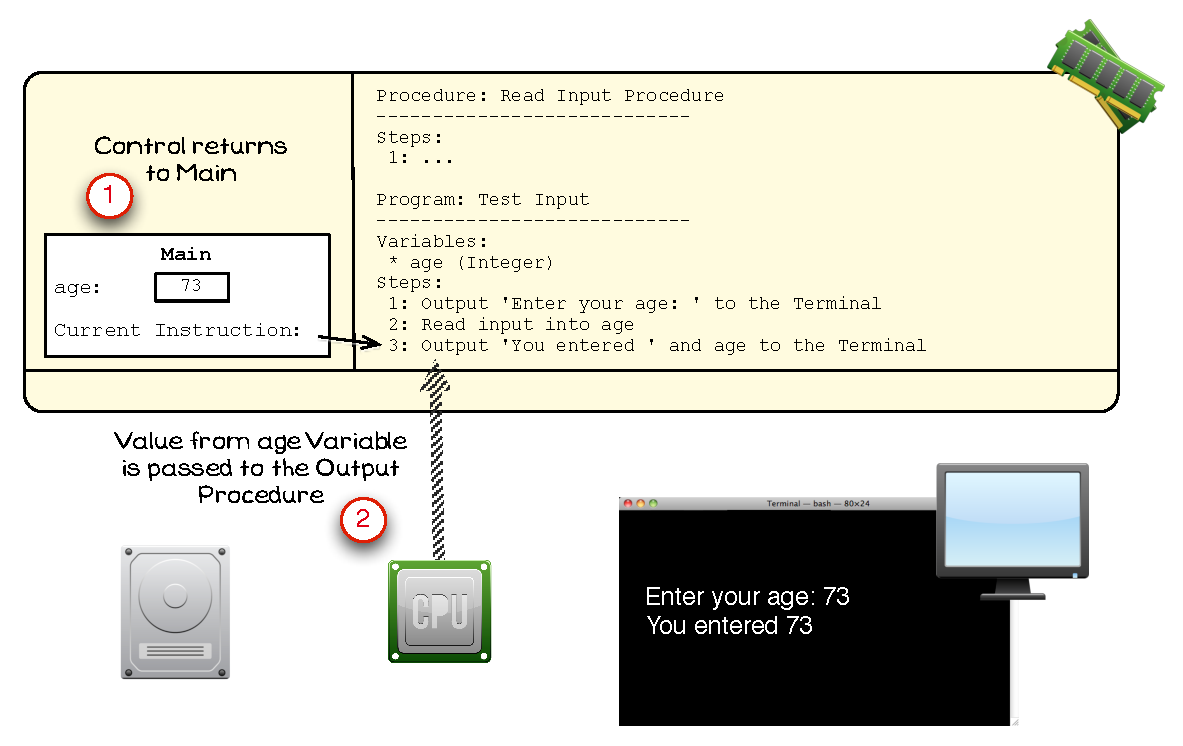
\includegraphics[width=\textwidth]{./topics/storing-using-data/images/vis-ref-4} 
   \caption{Control returns to Main, and the value of age has been updated by the input code}
   \label{fig:vis-ref-4}
\end{figure}

\mynote{
\begin{itemize}
  \item In Figure \ref{fig:vis-ref-4} the indicated areas show the following:
  \begin{enumerate}
    \item Control returns to \texttt{Main} when the input code completes.
    \item The \emph{value} from the \texttt{age} Variable is then passed to the Output procedure.
  \end{enumerate}
  \item \emph{Pass by Reference} is used when you want to pass the Variable, but in most cases you only want to pass the \emph{value} so most code uses \emph{Pass by Value}.
\end{itemize}
}

% subsubsection control_returns_to_main_and_ (end)
% subsection pass_by_reference (end)

\clearpage
\subsection{Hand Execution with Variables} % (fold)
\label{sub:hand_execution_with_variables}

One valuable skill you need to develop is the ability to step through a program in the same way the computer will. You will find that this skill will get more and more important as you progress to write larger programs. You will use this skill to help you detect and correct any \textbf{semantic errors}, in a process commonly referred to as \textbf{debugging}.

Semantic errors are errors in the logic of your program. This means that the program compiles, but does not do what you want it to. The tests that you use will help you locate these errors, but in many cases you will need to work out \emph{why} the error is occurring so that you can make the required changes.

One of the better techniques to help you make these corrections is to reading your code, and to think about the actions the computer is performing. Often these errors only require one or two lines of code to change, but before you can make these changes you need to identify \emph{where} the error is occurring, \emph{why} it is occurring, and \emph{how} you can correct the issue. By reading your code, and hand executing it you have the best chance of working out \emph{where} the problem is, and \emph{why} the problem is occurring.

These activities are very popular with Programming Tests, both in University subjects and job interviews. Being able to execute some code by hand means that you really understand what the code is doing. Once you have this level of understanding you just need to add some imagination and experience to become a very valuable software developer.

The steps you need to perform are:
\begin{itemize}
  \item \nameref{ssub:locate_the_function_or_procedure_to_test}
  \item \nameref{ssub:turn_off_your_brain}
  \item \nameref{ssub:setup_your_memory}
  \item \nameref{ssub:run_the_steps_one_at_a_time}
\end{itemize}

\subsubsection{Locate the Function or Procedure to Test} % (fold)
\label{ssub:locate_the_function_or_procedure_to_test}

Hand executing an entire program would take a very long time. As a result you want to narrow down your search to one or two Functions and/or Procedures. You can use your Structure Charts, or knowledge of the program's structure, to help you narrow down your options. Think about where the test failed, and where the code for this is located in your Program. With a small program you are likely to know immediately where the issue is, but as the program size grows it will become more difficult to know exactly where the problem is.

Listing \ref{plst:to-test} contains the pseudocode for a Procedure that will calculate and output the area of a Trapezoid. Unfortunately this code contains a number of errors. The following sections will demonstrate how to execute this procedure by hand. If this were a programming test you may be asked a question such as:
\begin{quote}
  `\emph{What is the value in area when this program is run and the user enters \textbf{5} for base 1, \textbf{7} for base 2, and \textbf{4} for height?}'
\end{quote}

Executing this by hand will give you the necessary skills to be able to answer questions such as this.

\pseudocode{plst:to-test}{Pseudocode for a Procedure that calculates the area of a Trapezoid, with errors.}{topics/storing-using-data/application/to-test.txt}

% subsubsection locate_the_function_or_procedure_to_test (end)

\subsubsection{Turn off your brain} % (fold)
\label{ssub:turn_off_your_brain}

Once you have located the Function or Procedure that you need to test you can start to execute it. The main obstacle in most peoples way is, unfortunately, their brain. You are going to \emph{think} about what you \emph{wanted} the program to do. This is something the computer \emph{cannot} do. The computer is unintelligent. It is a machine that does as you command. To run this program as the computer does you will need to \textbf{stop thinking} and start doing as commanded.

Rules:
\begin{itemize}
  \item Do not think about what you \emph{want} or \emph{expect} the program to do.
  \item Perform the commands as they are, one at a time
  \item You cannot remember anything that is not written down.
  \item Focus only on the current command (Statement). Do not look at other Statements!
  \item Perform the actions you are commanded to perform, and only those actions. Do not do more than you are commanded to.
  \item Use the language's Statements to determine the actions you must perform:
  \begin{itemize}
    \item An \nameref{sub:assignment_statement} will evaluate its expression, and assign a value to a variable.
    \item A \nameref{sub:procedure call} runs the code in a Procedure, a \nameref{sub:function_call} runs the code in a Function. To optimise this step you can perform the actions within called Functions or Procedures without stepping through their code in most cases.
  \end{itemize}
\end{itemize}

% subsubsection turn_off_your_brain (end)

\clearpage
\subsubsection{Setup your `memory'} % (fold)
\label{ssub:setup_your_memory}

One of the rules when running your code by hand is that you can not remember anything. The values you use must come from the `memory' that you setup for the Function or Procedure. So, the first step for executing this code performs the actions that called the procedure: you need to \emph{allocate space} on the stack. You can simulate this using a piece of paper. This piece of paper will be the `memory' used by the code as it executes. To set this memory up you will need to do the following:

\begin{enumerate}
  \item Get a blank piece of paper.
  \item Write \texttt{Print Trapezoid Area} to remember that is the procedure you are in.
  \item Do the following for any Variables\footnote{Draw boxes for Parameters, Local Variables, and Function results.} in the Function or Procedure:
  \begin{enumerate}
    \item \textbf{Draw a box} to represent the Variable. Make sure that it is large enough for you to write values inside.
    \item \textbf{Write the name} of the Variable next to the box.
    \item If the Variable is a Parameter, copy the value from the argument into the box, otherwise leave it empty.
  \end{enumerate}
\end{enumerate}

When you have finished these steps for the code in Listing \ref{plst:to-test} you should have a piece of paper that looks like the image in Figure \ref{fig:hand-exe-1}. The empty boxes represent the different Variables, the fact we have not written a Value into these boxes tells us that at this point the value has not been set, and therefore should not be used.

\begin{figure}[htbp]
   \centering
   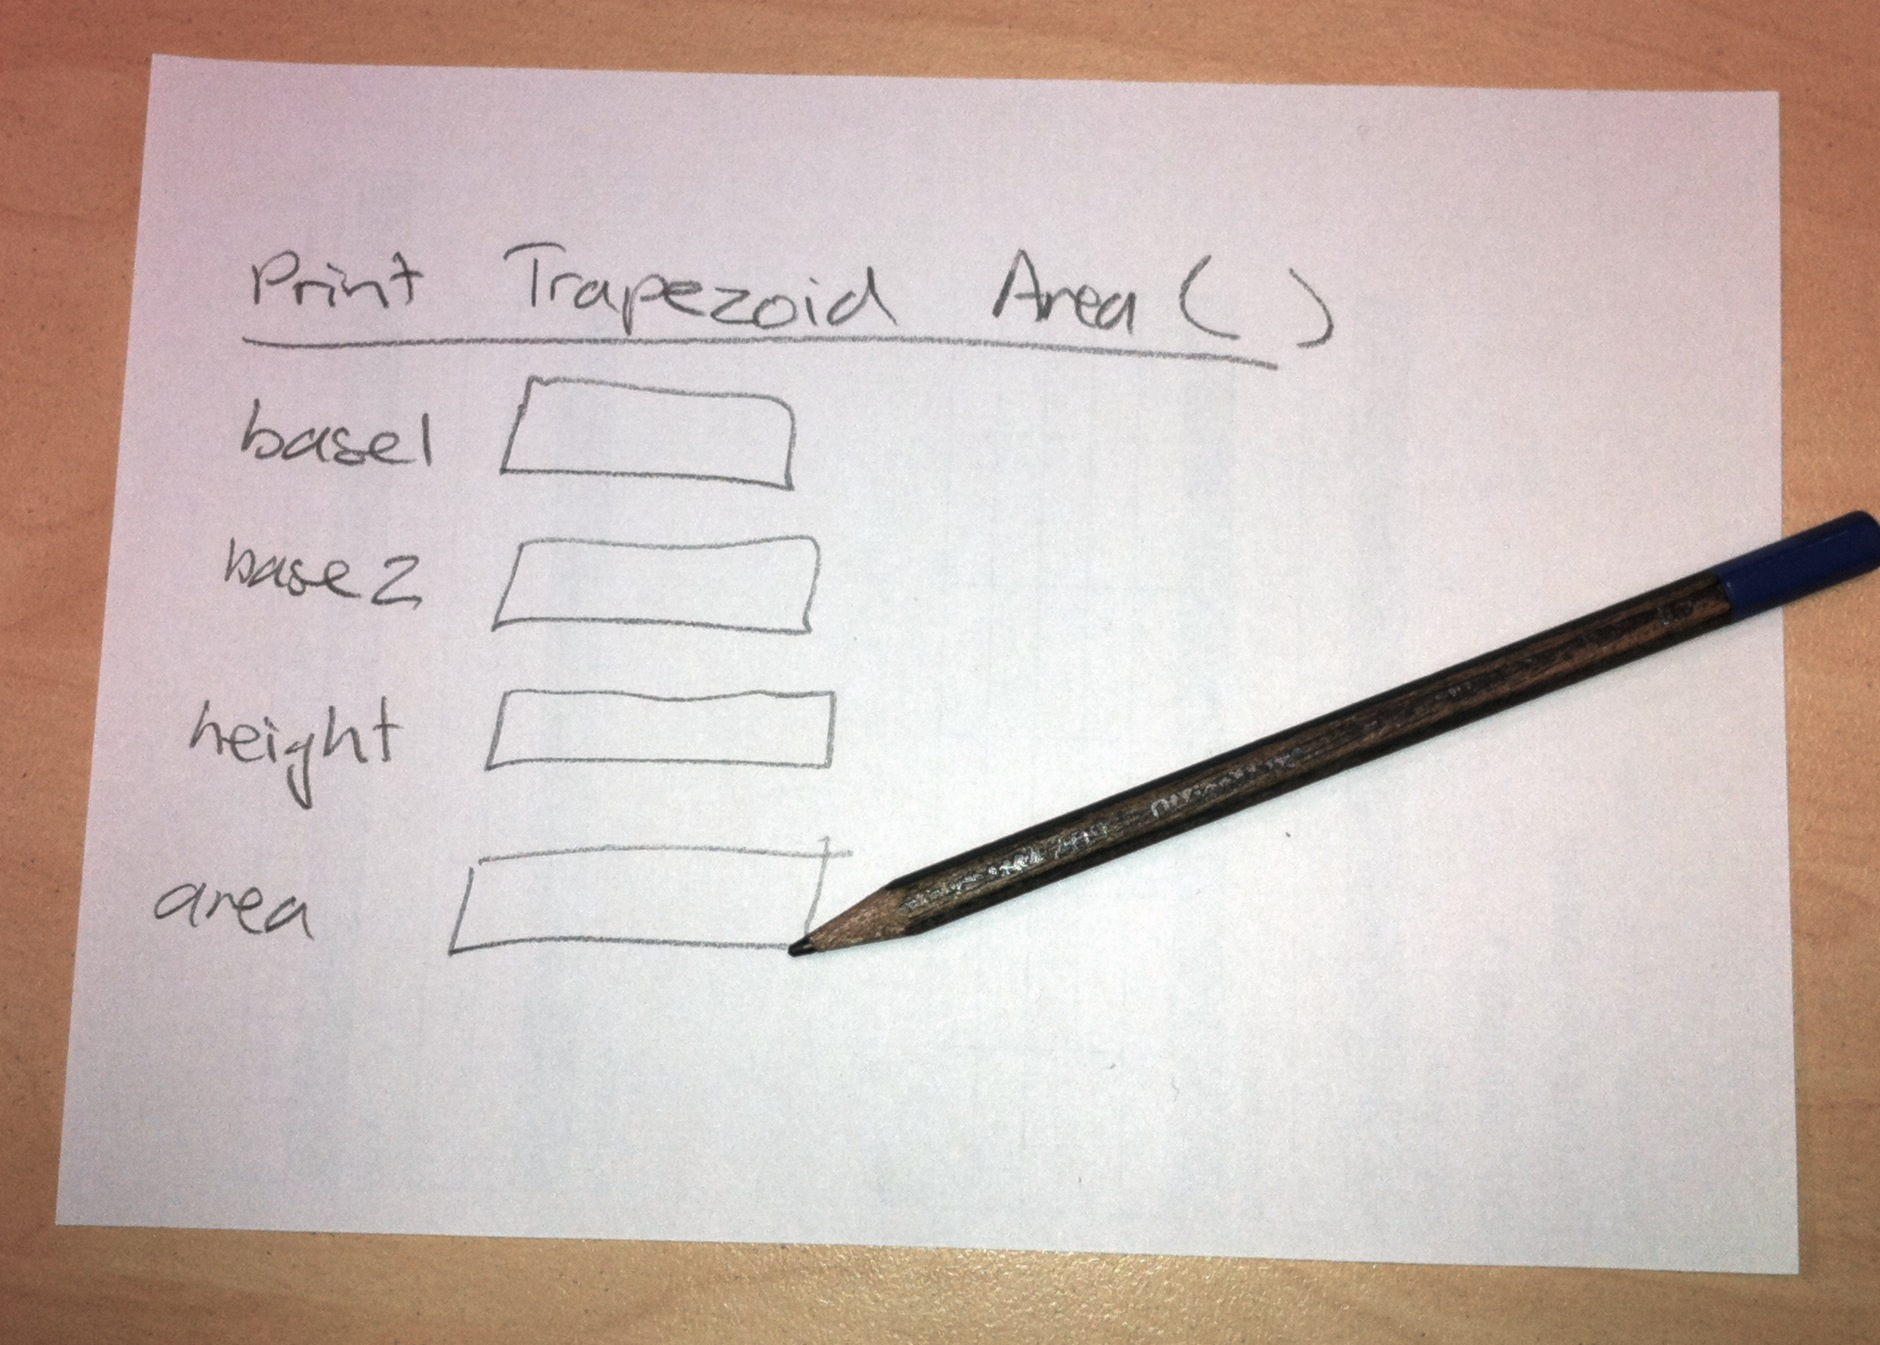
\includegraphics[width=0.7\textwidth]{./topics/storing-using-data/images/hand-exe-1} 
   \caption{Draw space for all of the Function or Procedure's Variables}
   \label{fig:hand-exe-1}
\end{figure}

% subsubsection setup_your_memory (end)

\clearpage
\subsubsection{Run the steps one at a time} % (fold)
\label{ssub:run_the_steps_one_at_a_time}

Now that the memory has been initialised it is time to run each instruction in the code. You need to do this \textbf{one instruction at a time}. It does not matter how large the code is, the computer will always run it one Statement at a time. Do not think, just read the Statement and perform the action.

\begin{enumerate}
  \item Step 1 calls the output procedure of the Language. This will output the text `\emph{Enter base 1: }' to the Terminal. You do not need to step into the internal actions of each Function or Procedure called, as long as you can replicate the actions that it would perform. If you had been asked `\emph{What is output by the the call to \texttt{Print Trapezoid Area}?}' it would be important to put this in the answer, but as we just want to know the final result you can skip this.
  \item Step 2 reads a value from the user and stores it in \texttt{base1}. The user is responding to the prompt from step 1, and therefore enters \emph{5}, the value indicated in the question. As the \texttt{base1} variable is passed to this call you now write \textbf{5} into the \texttt{base1} box, representing the fact that this Variable now has the value \emph{5}. See Figure \ref{fig:hand-exe-2}.
  \item Step 3 outputs the next prompt, `\emph{Enter base 2: }'.
  \item Step 4 reads a value from the user, and stores it in \textbf{\texttt{base1}}. This is the source of the first error. This is most likely the result of a copy/paste error, where the developer has copied the instructions to prompt the user and read a value into \texttt{base1}, and then changed it to read a value into \texttt{base2}. When you copy and paste code you need to pay extra attention to making sure that the pasted code is changed correctly.\newline\newline When this code is run a new value will be written into the \texttt{base1} Variable. Cross out the old value, and write in the new value. The value entered in this case is \textbf{7}, as indicated in the question. See Figure \ref{fig:hand-exe-3}.
  \item Step 5 outputs the prompt for height.
  \item Step 6 reads \textbf{4} from the user and stores it into the \texttt{height} Variable. See Figure \ref{fig:hand-exe-4}
  \item Step 7 now reads the values from \texttt{height}, and \texttt{base1}. The equation for calculating the area of a Trapezoid is $ height ( \frac{base 1 + base 2}{2} ) $, this has been coded incorrectly again, with several errors. Firstly \texttt{base1} is read twice, and \texttt{base2} is not used at all. Second, using BODMAS the current code is actually performing the equation $ height (base 1 + \frac{base 1}{2})$. Performing this calculation you will find that the value stored in \texttt{area} is $ 4 ( 7 + (7 / 2)) = 42$.
  \item Step 8 outputs the area to the Terminal, displaying `\emph{Trapezoid area is 42}'. See Figure \ref{fig:hand-exe-5}.
\end{enumerate} 

At this point the Procedure has ended, and you have collected all of the details about how the program actually works. You need to use this information to determine where the error is. If this failed to find the problem then the problem may be located elsewhere in the Program's code, or you have misread something. Getting someone else to help you debug your programs is always a good option, they are likely to see things that you may miss as the code's developer.

\mynote{
\begin{itemize}
  \item Pay careful attention to exactly what the statement is getting the computer to do.
  \item Proceed slowly and carefully, as mistakes can be as small as a single character in the wrong place.
  \item Make sure that you are aware of exactly what the different Statements do, and how they work.
  \item Always use the values of the Variables from `\emph{memory}', i.e. read/write them on to your piece of paper. 
\end{itemize}
}

\begin{figure}[htbp]
   \centering
   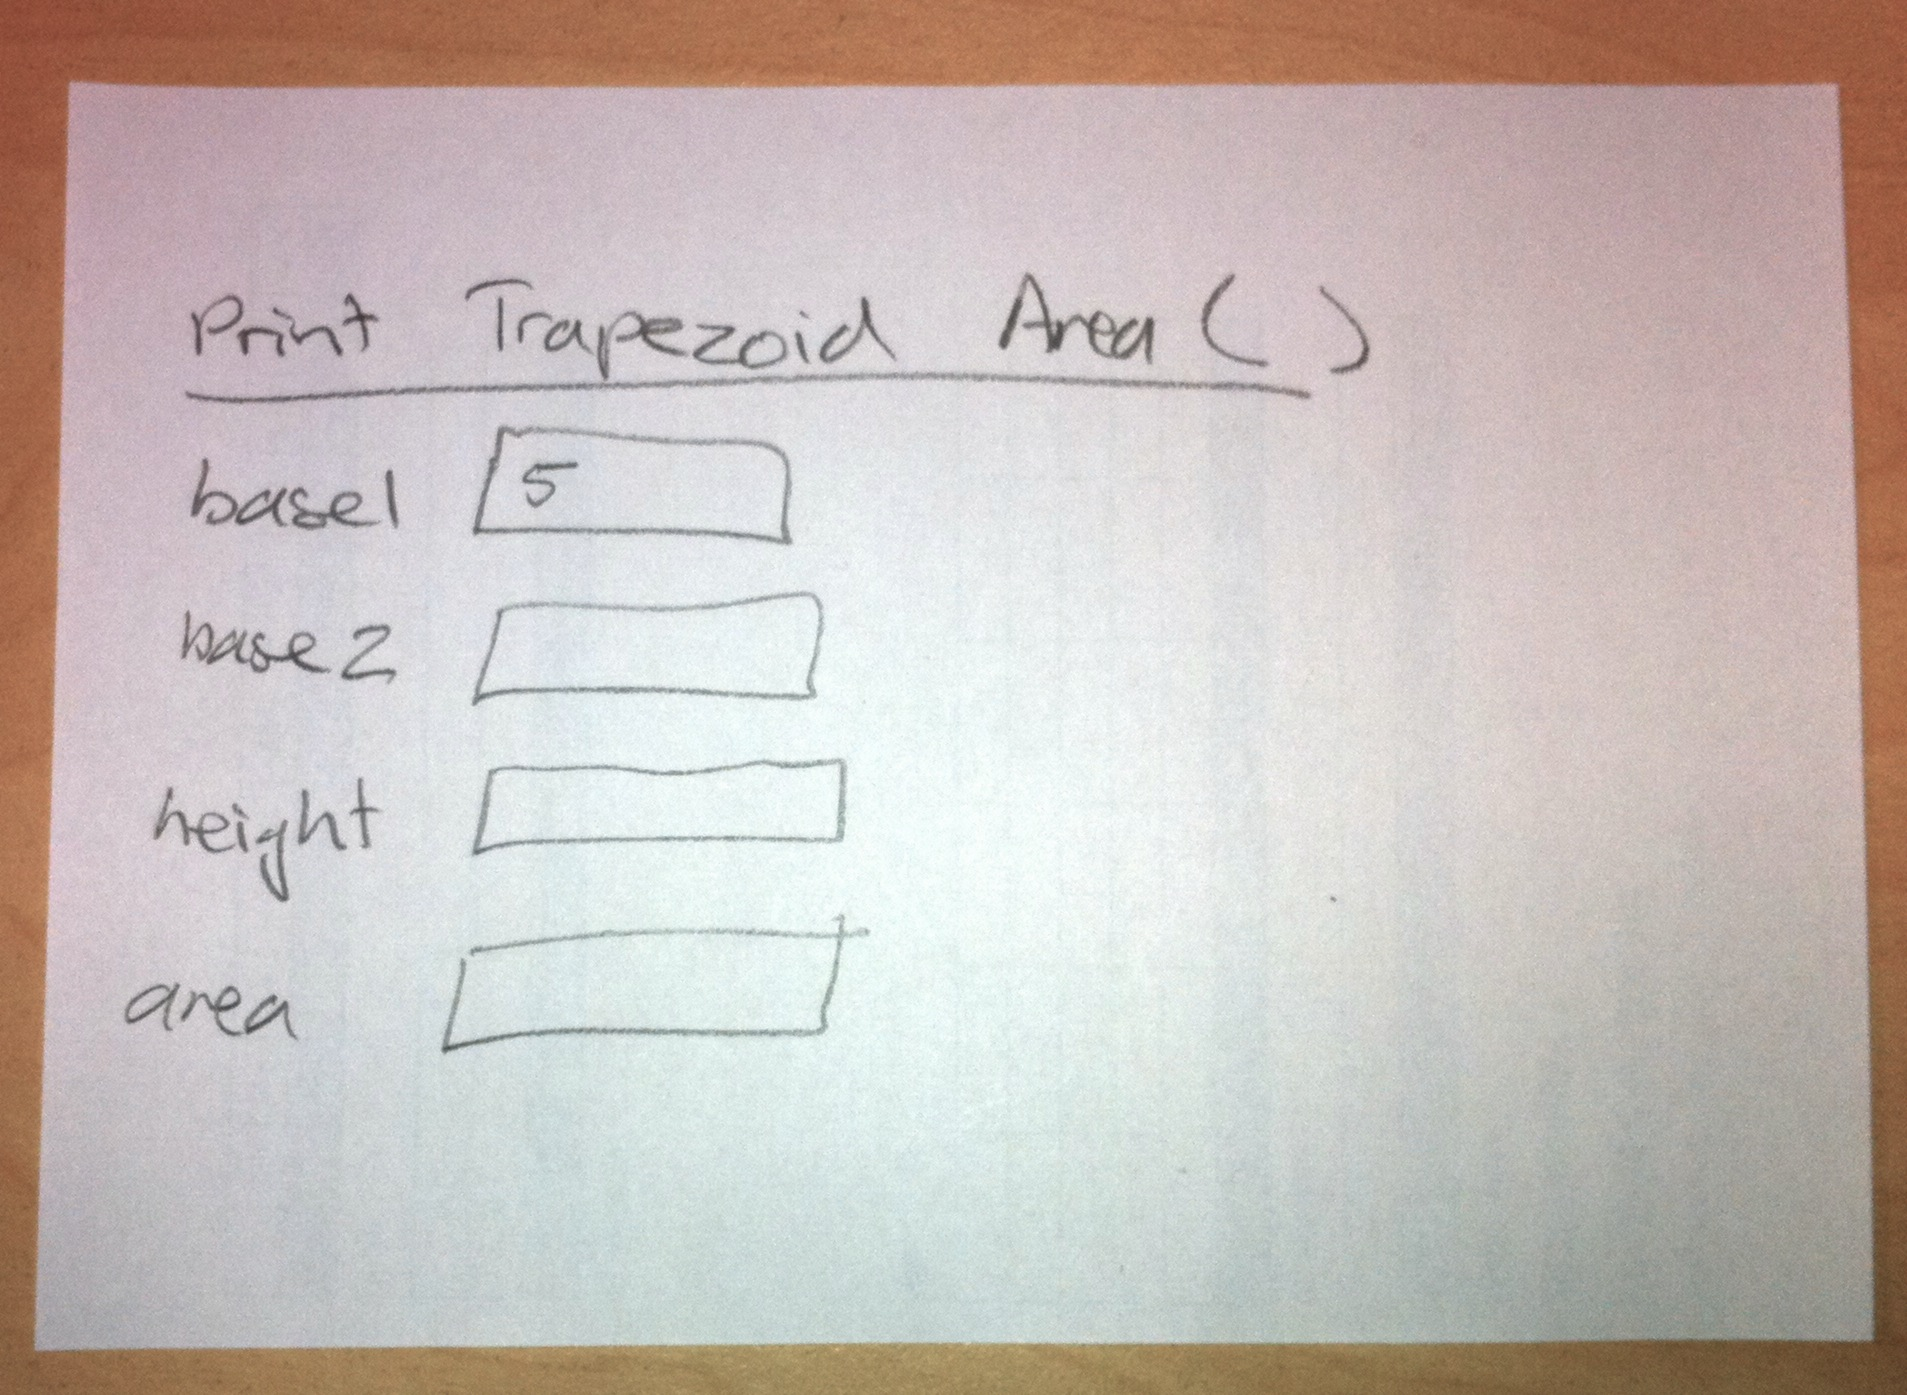
\includegraphics[width=0.7\textwidth]{./topics/storing-using-data/images/hand-exe-2} 
   \caption{The value 5 is stored in the \texttt{base1} Variable}
   \label{fig:hand-exe-2}
\end{figure}

\begin{figure}[htbp]
   \centering
   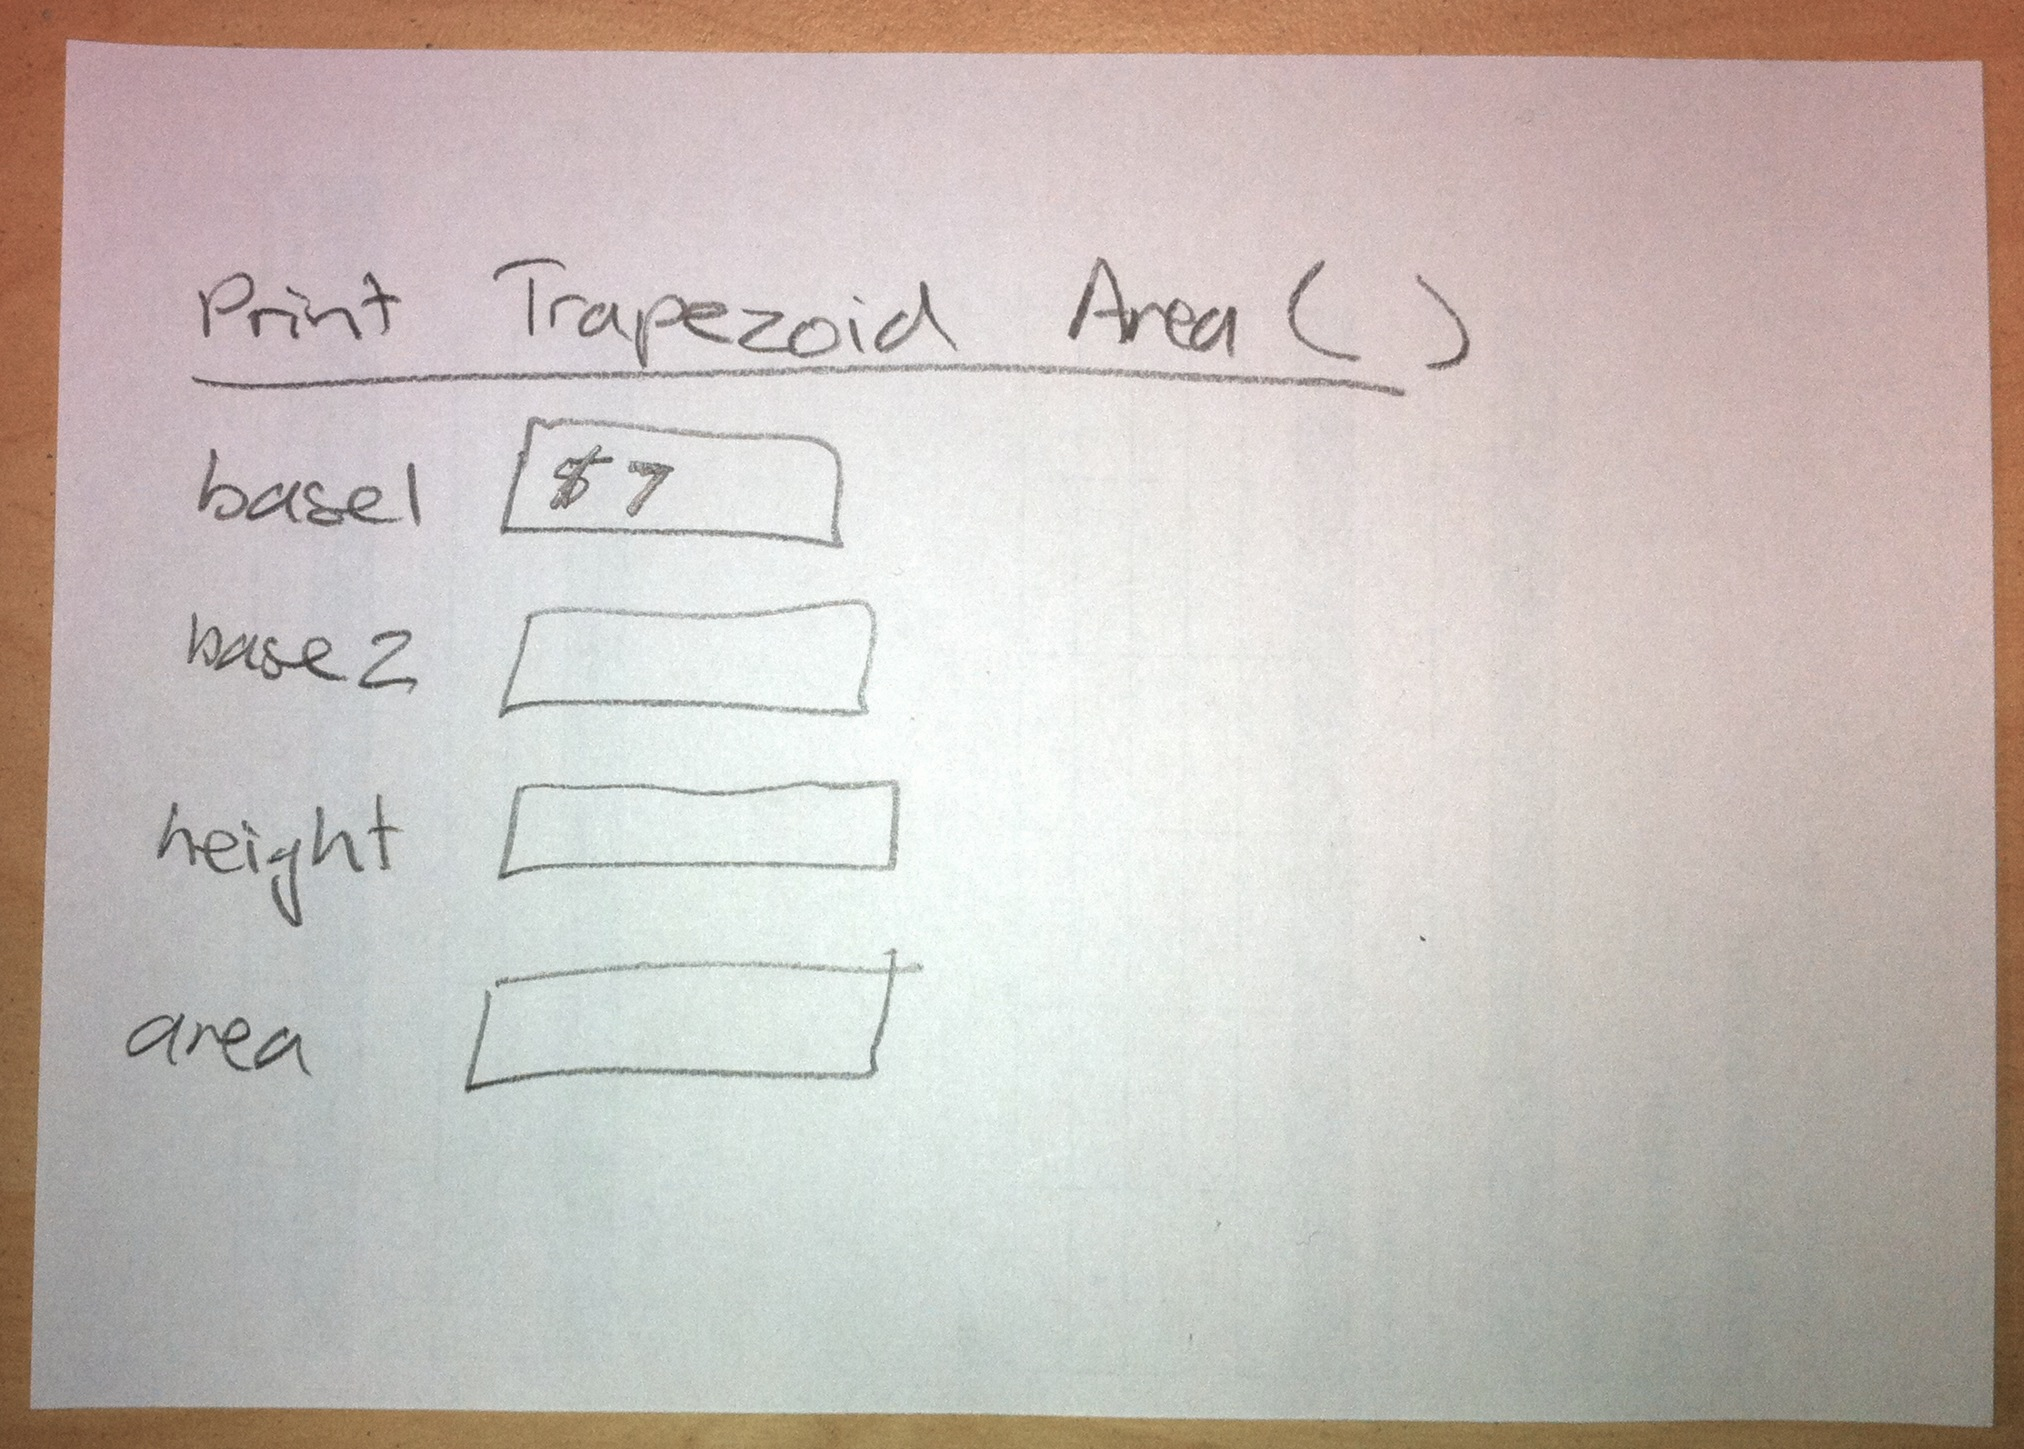
\includegraphics[width=0.7\textwidth]{./topics/storing-using-data/images/hand-exe-3} 
   \caption{The value 7 is stored in the \texttt{base1} Variable}
   \label{fig:hand-exe-3}
\end{figure}

\begin{figure}[htbp]
   \centering
   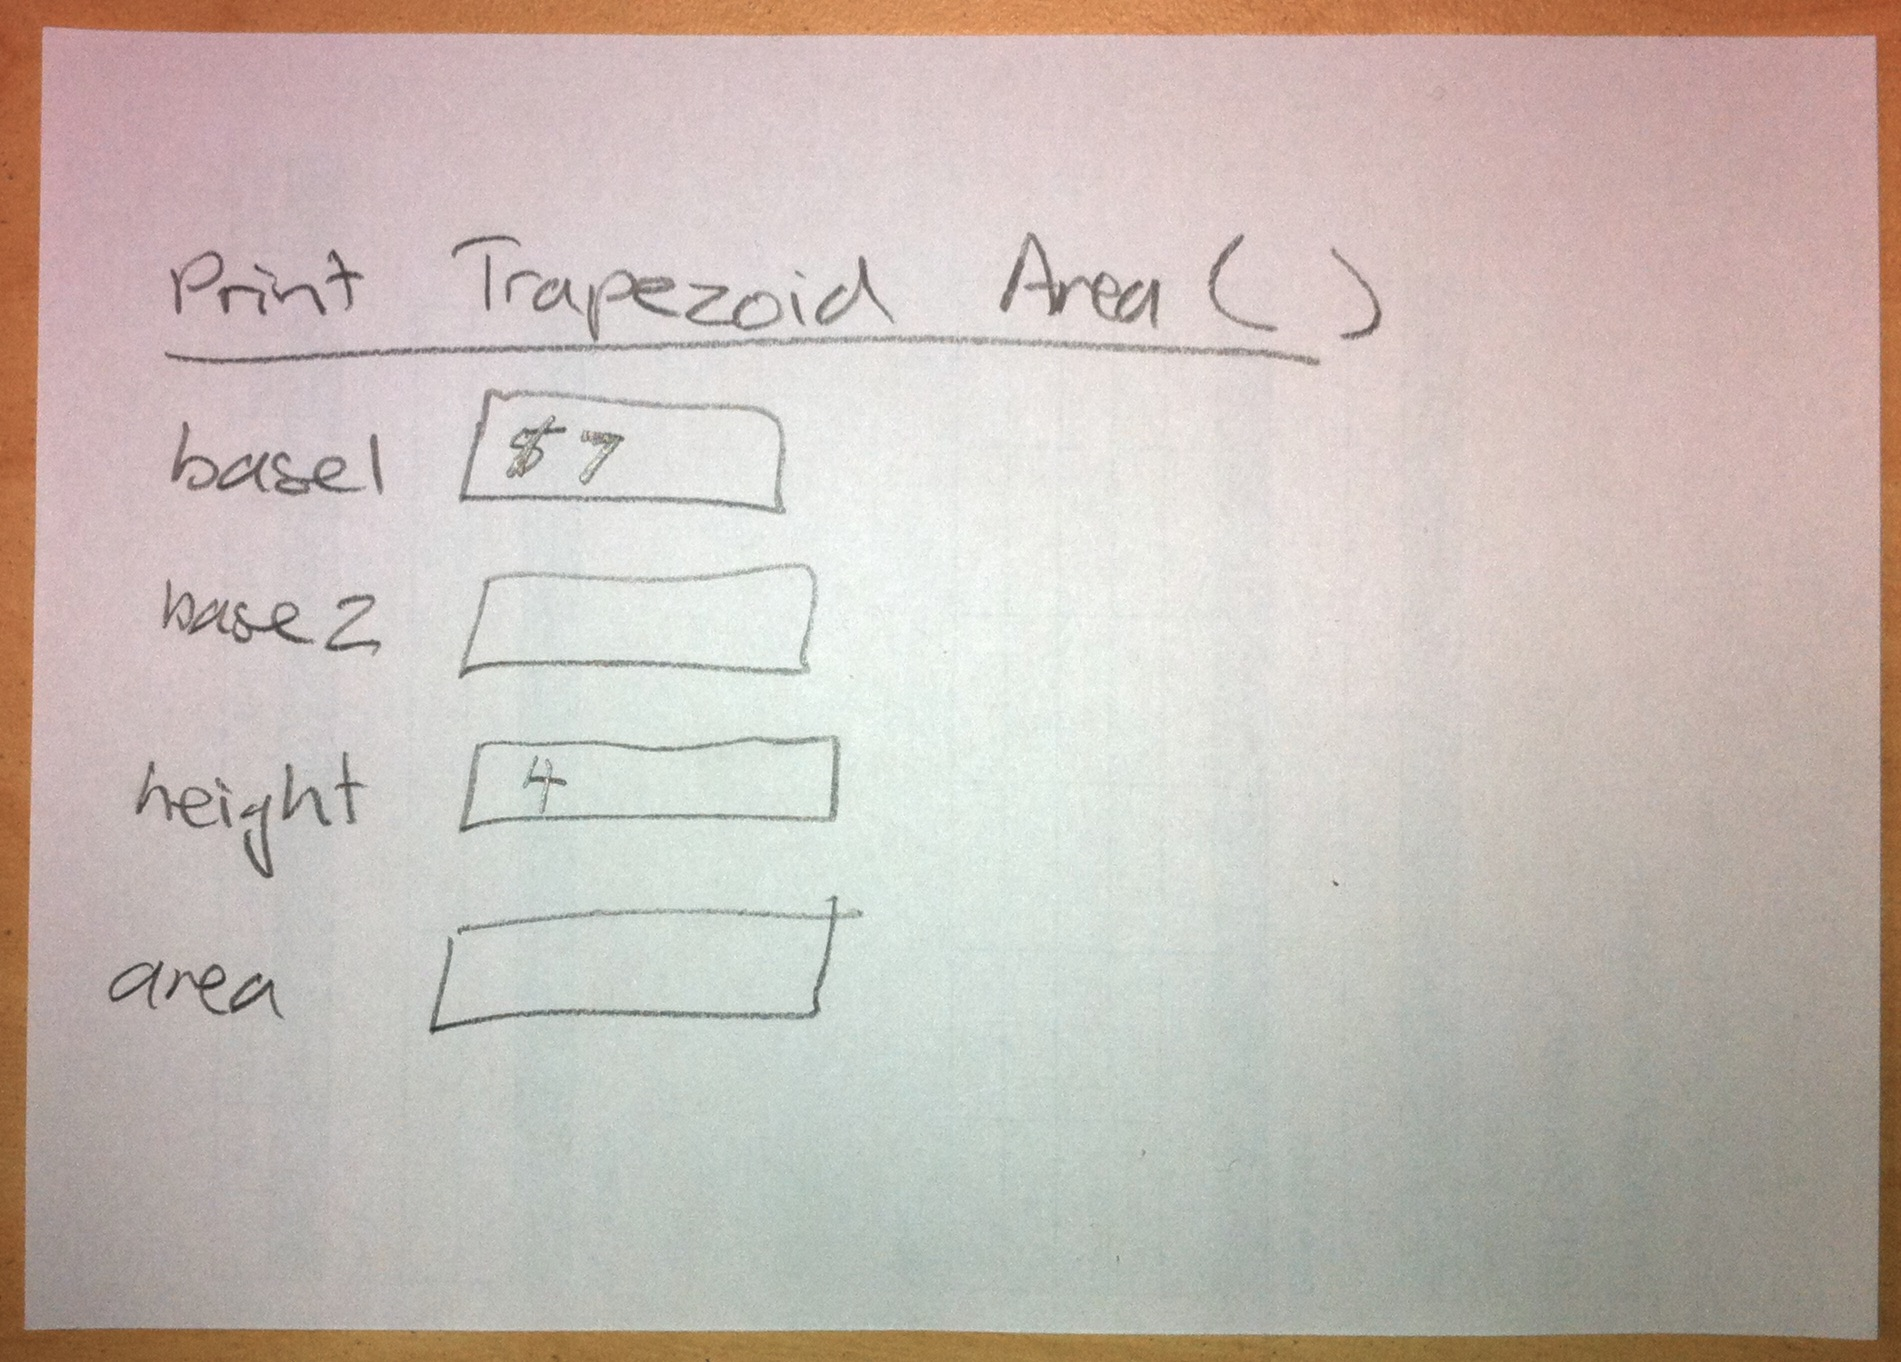
\includegraphics[width=0.7\textwidth]{./topics/storing-using-data/images/hand-exe-4} 
   \caption{The value 4 has been stored in \texttt{height}}
   \label{fig:hand-exe-4}
\end{figure}

\begin{figure}[htbp]
   \centering
   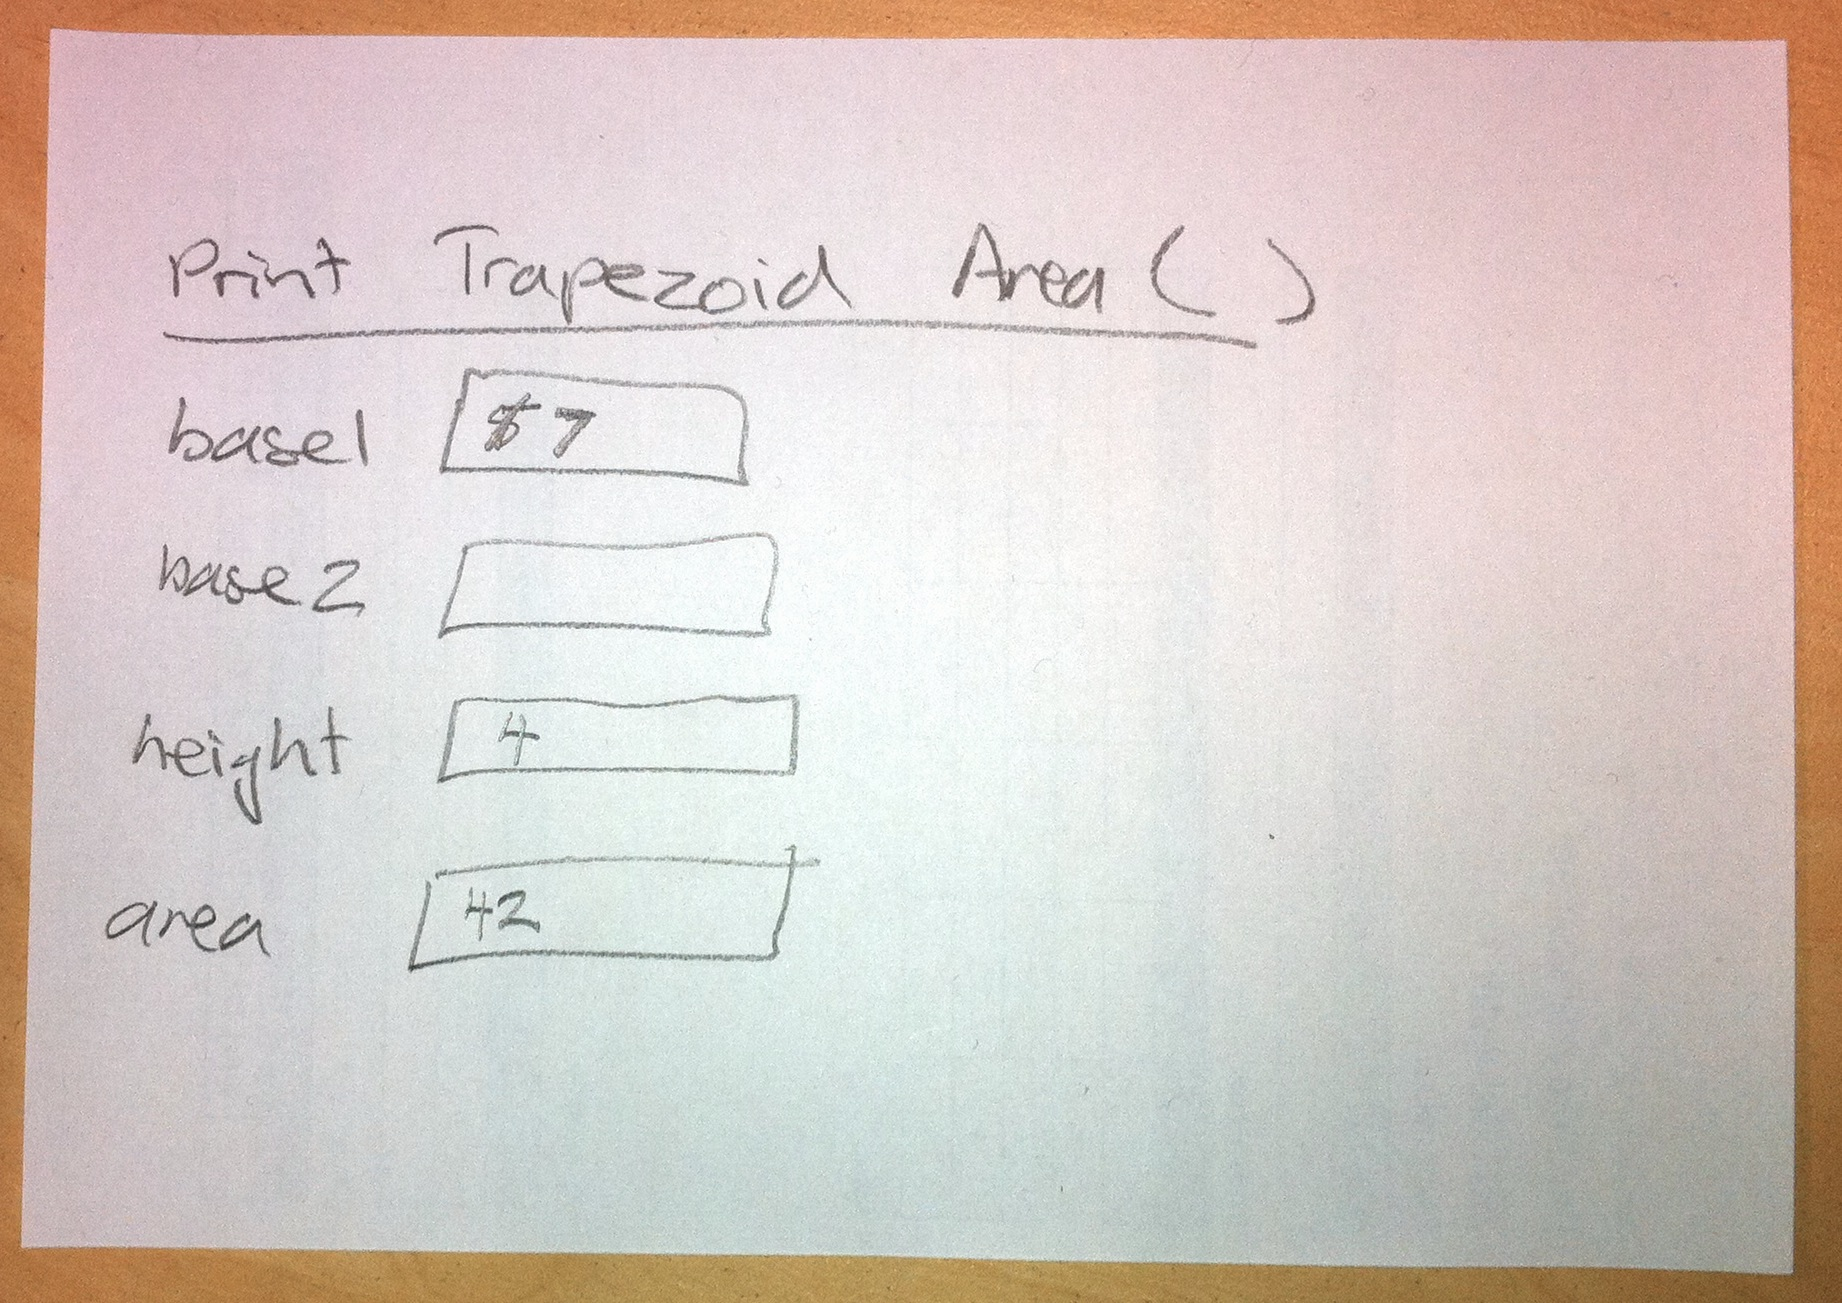
\includegraphics[width=0.7\textwidth]{./topics/storing-using-data/images/hand-exe-5} 
   \caption{The value 42 is stored in \texttt{area}}
   \label{fig:hand-exe-5}
\end{figure}

% subsubsection run_the_steps_one_at_a_time (end)
% subsection hand_execution_with_variables (end)

\clearpage
\subsection{Summary} % (fold)
\label{sub:visualise_data_summary}

In this Section you have seen how Variables work within the Computer, and been introduced to the idea of Functions. With these concepts you can now work more meaningfully with the data in your programs.

\bigskip
\mynote{
\begin{itemize}
  \item A Variable has two main aspects:
  \begin{itemize}
    \item The \textbf{Variable} itself, a space in memory. You can think of this like a box, into which a value can be placed.
    \item The \textbf{value} that is stored within the Variable.
  \end{itemize}
  \item Variables can be declared in one of three locations:
  \begin{itemize}
    \item \textbf{Local Variables} are declared within Functions and Procedures.
    \item \textbf{Parameters} are also declared within Functions and Procedures, but are given a value as part of the call to this code.
    \item \textbf{Global Variables} are declared within the Program, and are accessible within all Functions and Procedures.
  \end{itemize}
  \item The \textbf{Assignment Statement} can be used to store a value in a Variable. The \emph{left hand side} of an assignment is a Variable, the \emph{right hand side} is an Expression.
  \item You can read the \emph{value} of a Variable in an \textbf{Expression}.
  \item When you call a Function or a Procedure you can pass the Parameter either \textbf{by value} or \textbf{by reference}. When passed \emph{by reference} the Parameter must be passed a Variable.
  \item A \textbf{Function} is just like a Procedure, except that it returns a result and is therefore called inside Expressions so that the returned value can be used.
  \item A \textbf{Function} is called to \emph{calculate a value}.
\end{itemize}
}

% subsection summary (end)

% section understanding_dat (end)


% ====================
% = Examples Section =
% ====================
\clearpage
\section{Data Examples} % (fold)
\label{sec:data_examples}

\subsection{Times Table} % (fold)
\label{sub:times_table}

This program prints out the times table for a number entered by the user, displaying from 1 x n to 10 x n. The description of the program is in Table \ref{tbl:data-times-table}, the pseudocode in Listing \ref{lst:data-times-pseudo}, the C code in Listing \ref{lst:data-times-c}, and the Pascal code in Listing \ref{lst:data-times-pas}.

\begin{table}[h]
\centering
\begin{tabular}{l|p{10cm}}
  \hline
  \multicolumn{2}{c}{\textbf{Program Description}} \\
  \hline
  \textbf{Name} & \emph{Times Table} \\
  \\
  \textbf{Description} & Displays the Times Table from 1 x n to 10 x n. \\
  \hline
\end{tabular}
\caption{Description of the Times Table program}
\label{tbl:data-times-table}
\end{table}

\pseudocode{lst:data-times-pseudo}{Pseudocode for Times Table program.}{./topics/storing-using-data/examples/times-table.txt}

\mynote{
This is an updated version of the Seven Times Table Program. See Section \ref{sub:seven_times_table} \nameref{sub:seven_times_table}.
}

\clearpage

\csection{\ccode{lst:data-times-c}{C Times Table}{topics/storing-using-data/examples/times_table.c}}

\passection{\pascode{lst:data-times-pas}{Pascal Times Table}{topics/storing-using-data/examples/TimesTable.pas}}

% subsection times_table (end)

\clearpage
\subsection{Circle Area} % (fold)
\label{sub:circle_area_data}

This program prints out the area of a circle. The description of the program is in Table \ref{tbl:data-circle-area}, the pseudocode in Listing \ref{lst:data-circle-areas-pseudo}, the C code in Listing \ref{lst:data-circle-areas-c}, and the Pascal code in Listing \ref{lst:data-circle-areas-pas}.

\begin{table}[h]
\centering
\begin{tabular}{l|p{10cm}}
  \hline
  \multicolumn{2}{c}{\textbf{Program Description}} \\
  \hline
  \textbf{Name} & \emph{Circle Areas} \\
  \\
  \textbf{Description} & Displays the Circle Areas for circles with radius from 1.0 to 5.0 with increments of 0.5. \\
  \hline
\end{tabular}
\caption{Description of the Circle Areas program}
\label{tbl:data-circle-area}
\end{table}

\pseudocode{lst:data-circle-areas-pseudo}{Pseudocode for Circle Areas program.}{./topics/storing-using-data/examples/circle_areas.txt}

\mynote{
This is an updated version of the Circle Areas Program. See Section \ref{sub:circle_area} \nameref{sub:circle_area}.
}


\clearpage

\csection{\ccode{lst:data-circle-areas-c}{C Circle Areas}{topics/storing-using-data/examples/circle_areas.c}}

\passection{\pascode{lst:data-circle-areas-pas}{Pascal Circle Areas}{topics/storing-using-data/examples/CircleAreas.pas}}

% subsection circle_area (end)
\clearpage
\subsection{Bicycle Race} % (fold)
\label{sub:bicycle_race}

The Bicycle Race program will simulate a thirty second sprint race between a number of bicycles. The race has a standing start, and then each racer accelerates as fast as they can for thirty seconds. The winner is the racer who makes it the furthest.

\begin{itemize}
  \item You can calculate distance the racers cover using Equation~\ref{eq:acceleration}.
  \begin{itemize}
    \item \emph{s} is the distance covered.
    \item \emph{u} is the starting speed
    \item \emph{t} is time.
    \item \emph{a} is acceleration.
  \end{itemize} 
  \begin{equation}
    s = ut + \frac{a t^2}{2}
    \label{eq:acceleration}
  \end{equation}
  \item This race has a standing start, so the initial speed of each racer will be 0.
  \item The time for the race is 30 seconds, this is constant.
  \item Each racer will have a randomly determined acceleration, with a maximum acceleration of 10 $pixels/second^2$
\end{itemize}




\begin{table}[h]
\centering
\begin{tabular}{l|p{10cm}}
  \hline
  \multicolumn{2}{c}{\textbf{Program Description}} \\
  \hline
  \textbf{Name} & \emph{Comet Orbit} \\
  \\
  \textbf{Description} & Calculates and plots the position of the Hale-Bopp comet, based on an equation of its elliptical orbit of the sun. \\
  \hline
\end{tabular}
\caption{Description of the Comet Orbit program}
\label{tbl:data-comet-orbit}
\end{table}

\begin{figure}[p]
\csection{\ccode{clst:bike-race}{C Bicycle Race, continued in \lref{clst:bike-race1}}{topics/storing-using-data/examples/bike-race.c}}
\end{figure}

\begin{figure}[p]
\csection{\ccode{clst:bike-race1}{C Bicycle Race}{topics/storing-using-data/examples/bike-race1.c}}
\end{figure}


% subsection bicycle_race (end)

\clearpage
\subsection{Comet Orbit} % (fold)
\label{sub:comet_orbit}

This program uses SwinGame to draw the orbit of the Hale-Bopp comet around the sun. The Hale-Bopp comet performs an elliptical orbit of the sun that can be plotted using Equation~ \ref{eq:orbit}. This equation calculates the radius (r) of the comet's position based on the \emph{angle} between the comet and the sun. Where \emph{e} is the Eccentricity value with a constant value of 0.995, and \emph{d} is the distance between the pole and directrix with a constant value of 1.828.

\begin{equation}
  r = \frac{ed}{1 + e sin(angle)}
  \label{eq:orbit}
\end{equation}

\begin{table}[h]
\centering
\begin{tabular}{l|p{10cm}}
  \hline
  \multicolumn{2}{c}{\textbf{Program Description}} \\
  \hline
  \textbf{Name} & \emph{Comet Orbit} \\
  \\
  \textbf{Description} & Calculates and plots the position of the Hale-Bopp comet, based on an equation of its elliptical orbit of the sun. \\
  \hline
\end{tabular}
\caption{Description of the Comet Orbit program}
\label{tbl:data-comet-orbit}
\end{table}

This will require functions and procedures to do the following:
\begin{itemize}
  \item A function to \textbf{calculate} the \textbf{r} value for the comet based on an \emph{angle}.
  \item Functions to \textbf{convert} the \textbf{x} and \textbf{y} positions of the comet from AU (Astronomical Units) to pixel coordinates so that the comets position can be plotted on the screen.
  \item A procedure to \textbf{Draw} the \textbf{comet} to the screen, based on its current angle.
  \item A procedure to \textbf{Draw} the \textbf{sun}.
  \item A procedure to \textbf{draw} the entire \textbf{system}, including the sun and the comet at a given angle.
  \item The main procedure to coordinate actions (calling, draw system with different angle values).
\end{itemize}

\clearpage

\csection{\ccode{clst:comet-orbit}{Comet Orbit, continued in \lref{clst:comet-orbit1}}{topics/storing-using-data/examples/comet-orbit.cpp}}

\begin{figure}[p]
\csection{\ccode{clst:comet-orbit1}{Comet Orbit, continued in \lref{clst:comet-orbit2}}{topics/storing-using-data/examples/comet-orbit1.cpp}}
\end{figure}

\begin{figure}[p]
\csection{\ccode{clst:comet-orbit2}{Comet Orbit}{topics/storing-using-data/examples/comet-orbit2.cpp}}
\end{figure}

% subsection comet_orbit (end)


% section data_examples (end)

% =============
% = Exercises =
% =============
\clearpage
\section{Data Exercises} % (fold)
\label{sec:data_exercises}

Read over the concepts in this chapter and answer the following questions:
\begin{enumerate}
  \item What is a \nameref{sub:variable}?
  \item What is the relationship between a variable and a value?
  \item What is the relationship between a variable and a type?
  \item Where can you use variables? Think both reading the value, and storing a new value.
  \item What does it mean if a variable appears on the right hand side of an assignment? What will happen to this variable when the code is run?
  \item What does it mean if a variable appears on the left hand side of an assignment? What will happen to this variable when the code is run?
  \item What is a \nameref{sub:constant}? How does it differ from a variable?
  \item What is a local variable? What code can access the value in a local variable?
  \item What is a global variable? What code can access the value in a global variable?
  \item Why is it considered good practice to use local variable, but not global variables?
  \item How do parameters help make procedures more powerful?
  \item What are the two parameter passing mechanisms for passing parameters? How are they different?
  \item When would you use each of the parameter passing mechanisms? For what kind of parameters?
  \item How does the Terminal input procedure store a value in the variable you pass to it? What kind of parameter passing is involved here?
  \item What statement was introduced in this chapter?
  \item What does this statement allow you to do?
  \item What is a function? How does it differ from a procedure?
  \item A procedure call is a statement. What is a function call? Why is this different?
  \item What does it mean when you say a function returns a value? 
  \item What are the values of the following expressions?
  
  \begin{table}[h]
    \centering
    \begin{tabular}{|c|l|l|}
      \hline
      \textbf{Question} & \textbf{Expression} & \textbf{Given} \\
      \hline
      (a) & \texttt{5} & \\
      \hline
      (b) & \texttt{a} & \texttt{a} is 2.5 \\
      \hline
      (c) & \texttt{1 + 2 * 3} & \\
      \hline
      (d) & \texttt{a + b} & \texttt{a} is 1 and \texttt{b} is 2 \\
      \hline
      (e) & \texttt{2 * a} & \texttt{a} is 3 \\
      \hline
      (f) & \texttt{a * 2 + b} & \texttt{a} is 1.5 and \texttt{b} is 2\\
      \hline
      (g) & \texttt{a + 2 * b} & \texttt{a} is 1.5 and \texttt{b} is 2 \\
      \hline
      (h) & \texttt{(a + b) * c} & \texttt{a} is 1, b is 1 and \texttt{c} is 5 \\
      \hline
      (i) & \texttt{a + b * 2} & \texttt{a} is 1.0 and \texttt{b} is 2\\
      \hline
    \end{tabular}    
  \end{table}
\end{enumerate}


\clearpage
Apply what you have learnt to the following tasks:
\begin{enumerate}
  \item Take the times table program from \sref{sub:times_table} and re-implement it so that there are two procedures: \texttt{Print Times Table}, and \texttt{Print Times Table Line}. Use these to print the 42, 73, and 126 times tables, as well as printing a times table the user requests.
  \begin{itemize}
    \item The \texttt{Print Times Table Line} procedure will take two parameters. The first will be the number, the second will be the times. This will output a single line for the table, e.g. ` 1 x 73 = 73'. 
    \item The \texttt{Print Times Table} procedure will have a single parameter called \texttt{number}. It will output a header for the table, and then call \texttt{Print Times Table Line} ten times. In each call it will pass 1, 2, 3, etc. for the times parameter, and pass across its \texttt{number} value to the \texttt{number} parameter. After printing the last line it will output a footer for the table.
  \end{itemize}
  \item Correct and then implement the Trapezoid Area procedure from \sref{sub:hand_execution_with_variables}. Adjust the implementation to call a \texttt{Trapezoid Area} function that is passed the two base values and the height, and returns the area. Create a small program to test this procedure.
  \item Implement the Change Calculation program, and test it function as you expect.
  \item Revisit your Circle Dimensions program from \cref{cha:program_creation} and adjust its implementation to make use of functions and procedures.
  \item Design the structure and then the code for a program that converts temperatures from Celsius to Fahrenheit. This should read the value to convert from the user, and output the results to the Terminal.
  \item Take the adjusted Face Shape program from \cref{cha:procedure_declaration}, and re-implement it so that the \texttt{Draw Face} procedure takes in an x and y coordinate for the location where the face will be drawn. Adjust the coordinates of the face's components in \texttt{Draw Face}, by the amounts in the \texttt{x} and \texttt{y} parameters. Use your new procedure to draw three faces to the screen at different positions.
  \item Write a \texttt{Swap} procedure that takes in two integer parameters (passed by reference) and swaps their values. Write a program to test this procedure. This should work so that if you call \texttt{Swap(a, b);} that the values in the \texttt{a} and \texttt{b} variables are swapped over. You can test this by printing the values before and after the call to the \texttt{Swap} procedure.
  \item Write a small program to experiment with parameter passing. Create in this program a procedure called \texttt{Print It} that takes a integer parameter and prints it to the Terminal. Also create a  \textbf{Double It} procedure that takes an integer parameter passed by reference\footnote{If you are using C, you will need to do this with C++. With C++ your compiler is now g++, rather than gcc.} and has its value doubled in the procedure. Try the following (not all will work):
  \begin{enumerate}
    \item Call \texttt{Print It}, passing in a literal value like \texttt{5}.
    \item Call \texttt{Double It}, passing in a literal value like \texttt{5}.
    \item Call \texttt{Print It}, passing in a calculated expression like \texttt{a + b}.
    \item Call \texttt{Double It}, passing in a calculated expression like \texttt{a + b}.
    \item Call \texttt{Print It}, passing in a variable's value.
    \item Call \texttt{Double It}, passing in a variable's value.
  \end{enumerate}
  
  \clearpage
  \item Watch \url{http://www.youtube.com/watch?v=y2R3FvS4xr4}, which clearly demonstrates the importance of being able to calculate the airspeed velocity of a swallow. This can be calculated using an equation based on the Strouhal Number, see \url{http://www.style.org/strouhalflight}. Use this information to create a program that can be used to calculate the airspeed velocity of African and European Swallows. Use the following values:
  \begin{itemize}
    \item Strouhal Number of 0.33
    \item African Swallow: frequency 15hz, amplitude 21cm
    \item European Swallow: frequency 14hz, amplitude 22cm
  \end{itemize}
\end{enumerate}

\bigskip

If you want to further your knowledge in this area you can try to answer the following questions. The answers to these questions will require you to think harder, and possibly look at other sources of information.

\begin{enumerate}
  \item Further adjust your Face Drawing program so that the caller can pass in a custom color, width, and height for the face.
  
\end{enumerate}



% section data_exercises (end)

% ===========
% = Project =
% ===========
% \clearpage
% \section{Data in the Project} % (fold)
% \label{sec:data_in_the_project}

% section data_in_the_project (end)


% chapter storing_and_using_data (end)